% An MSI thesis template thrown together Oct 2005 - CW


\documentclass[a4paper,12pt]{book}


  % a file containing your definitions, which packages to load etc
  % Bibliography
\usepackage[
	hyperref=true,
	url=false,
	isbn=false,
	style=alphabetic,
	citereset=chapter,
	maxcitenames=3,
	maxbibnames=10,
	block=none]{biblatex}
\addbibresource{bibliography.bib}
\AtEveryBibitem{\clearfield{note}}

% Remove extraneous fields from bibliography.
\AtEveryBibitem{
	\clearfield{howpublished}
	\clearfield{pagetotal}
}

% Math
\usepackage{amsmath}
\usepackage{amsthm}
\usepackage{amssymb}
\usepackage{amsfonts}
\usepackage{dsfont}
\usepackage{mathrsfs}

\usepackage{tikz-cd}
\usepackage{tikz}
\usepackage{mathtools}

% Detecting if table is in math mode.
% Typesetting everything in table in math mode if so.
\usepackage{tabu}

% Colored links.
\usepackage{color}
\usepackage{xcolor}
\usepackage{hyperref}
\hypersetup{
	colorlinks,
	linkcolor={red!50!black},
	citecolor={blue!50!black},
	urlcolor={blue!80!black}
}
\usepackage{hyperref}
\usepackage{url}

\usepackage{graphicx}
\usepackage{subcaption}
\usepackage{enumerate}
\usepackage{wrapfig}
\usepackage [english]{babel}
\usepackage [autostyle, english = american]{csquotes}
\MakeOuterQuote{"}
\usepackage{epigraph}

% to make todo 
\usepackage{todonotes}

\graphicspath{{img/}}



% some theorem environments
% remove "[theorem]" if you do not want them to use the same number sequence
  \newtheorem{theorem}{Theorem}[chapter]
  \newtheorem{lemma}[theorem]{Lemma}
  \newtheorem{prop}[theorem]{Proposition}
  \newtheorem{cor}[theorem]{Corollary}

  \newtheorem{conj}[theorem]{Conjecture}

  \theoremstyle{definition}
  \newtheorem{defn}[theorem]{Definition}
  \newtheorem{conv}[theorem]{Convention}
  \newtheorem{ex}[theorem]{Example}
  \newtheorem{exs}[theorem]{Examples}
  \newtheorem{question}[theorem]{Question}
  \newtheorem{remark}[theorem]{Remark}
  \newtheorem{notn}[theorem]{Notation}

% esssup
\DeclareMathOperator*{\esssup}{ess\,sup}
\DeclareMathOperator*{\argmin}{arg\,min}
\DeclareMathOperator*{\cl}{cl}
\DeclareMathOperator*{\co}{co}
\DeclareMathOperator*{\dom}{dom}
\newcommand{\overbar}[1]{\mkern 1.5mu\overline{\mkern-1.5mu#1\mkern-1.5mu}\mkern 1.5mu}
\DeclareMathOperator*{\simd}{\stackrel{\text {d}}{\sim}}
\DeclareMathOperator*{\disteq}{\stackrel{\text {d}}{=}}
\DeclareMathOperator*{\distconv}{\stackrel{\text {d}}{\to}}
\DeclareMathOperator*{\probconv}{\stackrel{\text {Pr}}{\to}}
\DeclareMathOperator*{\asconv}{\stackrel{\text {a.s.}}{\rightarrow}}
\DeclareMathOperator{\erf}{erf}
\DeclareMathOperator{\erfc}{erfc}

\newcommand{\E}{\ensuremath{\mathbb{E}}}
\newcommand{\sumn}{\ensuremath{\sum_{i = 1}^n}}
\newcommand{\Ca}{\ensuremath{\operatorname{CVaR}_\alpha}}
\newcommand{\LL}{\ensuremath{\mathscr{L}}}
\newcommand{\cvar}{\ensuremath{\operatorname{CVaR}}}
\newcommand{\evar}{\ensuremath{\operatorname{EVaR}}}
\newcommand{\var}{\ensuremath{\operatorname{VaR}}}
\newcommand{\loss}{\ensuremath{\operatorname{Loss}}}


\DeclarePairedDelimiter\ceil{\lceil}{\rceil}
\DeclarePairedDelimiter\floor{\lfloor}{\rfloor}


  % line-spacing factor
  \renewcommand{\baselinestretch}{1.2}

  % use this if you don't want headers and page numbers on
  % blank pages at the end of chapters
  \newcommand{\blanknonumber}{\newpage\thispagestyle{empty}}

  % needed for ANU logo on titlepage (optional)
  \usepackage{graphics}

  % margins
  \setlength{\voffset}{-1in}
  \setlength{\hoffset}{-1in}
  \setlength{\oddsidemargin}{4cm}
  \setlength{\evensidemargin}{2.5cm}
  \setlength{\textwidth}{14.5cm}
  \setlength{\textheight}{22.5cm}
  \setlength{\topmargin}{2.5cm}


  % for working drafts, un-comment the following command and list
  % the chapters etc you want to see in the output, eg
  % \includeonly{titlepage,chapter1,chapter2}



\begin{document}


  % set page numbers to roman and suppress chapter numbers
  \frontmatter


  % remove or switch the order of these as you see fit
  \begin{titlepage}
\begin{center}

\vspace*{\fill} \Huge
                        Beyond Expectations, But Within Limits --- The Theory of Coherent Risk Measures
\\
\vfill\vfill\Large
                          Yuxi Liu
\\
\vfill\vfill
                          October 2019
\\
\vfill\vfill \normalsize
         A thesis submitted for the degree of Bachelor of Science (Advanced) (Honours)\\
         of the Australian National University
\vfill
         
\includegraphics{ANU.eps}

\end{center}

\end{titlepage}
\blanknonumber
  

\blanknonumber\ \blanknonumber

\vspace*{\fill}

\begin{center}\emph{
%
For the glory of Celestia,\\
And Her dominion come.
%
}
\end{center}

\vfill\vfill\vfill
\blanknonumber
  
\chapter*{Declaration}\label{declaration}
\thispagestyle{empty}
The work in this thesis is my own except where otherwise stated.

\vspace{1in}


\hfill\hfill\hfill
%
Yuxi Liu
%
\hspace*{\fill}
\blanknonumber
  
\chapter*{Acknowledgements}\label{acknowledgements}
\addcontentsline{toc}{chapter}{Acknowledgements}

I would like to thank the following people for the successful completion of my thesis.

Main supervisor, Robert Williamson, who used his knowledge in the fields of risk measure and philosophy to give valuable guidance for me. The weekly meetings were vital for keeping me afloat in an unfamiliar ocean of knowledge.

Co-supervisor, Markus Hegland, who, while I have not met for many times, gave good feedback during the writing phase of my thesis.

My parents, who gave unwavering material support.

Best friends, Artline, Ira, and Lurid, who kept me alive during the years.\blanknonumber
  \chapter*{Abstract}\label{abstract}

\addcontentsline{toc}{chapter}{Abstract}


Expectation lies at the foundation of probability, but its centrality belies its contingency. Abstractly, the expectation of a random variable is a real number that measures some information about the variable, and one may well explore the consequences of replacing expectation by some alternative.

Certain alternatives to expectation, termed "coherent risk measures", have been well-investigated in financial engineering, but they are relatively unknown in the field of machine learning. Here, we collect and prove some fundamental properties of coherent risk measures that we believe would be applicable to machine learning.

In Chapter 1, we give a guide to the thesis, then we review the concept of risk measures, point out possible deficiencies of the expectation as a risk measure, and provide a historical overview of the study of risk measures in finance and other areas.

In Chapter 2, we review basic probability concepts, then define the concept of coherent risk measures and study the geometric properties of their envelope representations. Armed with geometric insight, we prove a Kusuoka representation theorem when the underlying sample space is finite and uniform, and construct counterexamples when it is finite but nonuniform.

In Chapter 3, we generalize some basic probability inequalities and concentration inequalities from expectation to conditional value at risk. Then we review statistical learning theory and generalize its basic concepts and its fundamental theorem by replacing expectation with spectral risk measures.

In Chapter 4, we review limit theorems in probability, give a new and intuitive proof of the central limit theorem for the empirical estimator of CVaR. We also prove the uniform strong law of large numbers for the empirical estimator of spectral risk measures. We provide numerical evidence to support our results and generate conjectures.

In Chapter 5, we summarize the main theorems and conjectures of the thesis, review the literature on applications of general risk measures to machine learning, and point to possible future research directions.\blanknonumber
  \tableofcontents\blanknonumber
  

\chapter{Notation, convention, and terminology}\label{notation}
%\addcontentsline{toc}{chapter}{Notation and terminology}

\renewcommand{\thefootnote}{\fnsymbol{footnote}}

\

\noindent\textbf{Notation and convention}

% adjust the lengths to suit your needs (difference of .22cm works best)

Conventions are choices that are purely for convenience and disambiguation, with no deep significance.

\newcommand{\nttn}[2]{\item[{\ \makebox[3.18cm][l]{#1}}]{#2}}
\begin{list}{}{ \setlength{\leftmargin}{3.4cm}
                \setlength{\labelwidth}{4.8cm}}

\nttn{$\mathbb{N}$}{The set of natural numbers is $\{1, 2, ...\}$.}

\nttn{$n$}{A positive integer, unless otherwise noted.}

\nttn{$[n]$}{$\{1, 2, ..., n\}$, with caveat that $n \ge 1$}

\nttn{$c$}{A real constant, unless otherwise noted.}

\nttn{$x^+$}{Positive part of $x$, that is, $\max(x, 0)$.}

\nttn{$\partial A$}{Topological boundary of $A$.}

\nttn{$\cl(A)$}{The topological closure of $A$.}

\nttn{$\co(A)$}{The convex hull of $A$, where $A$ is a subset of some real vector space.}

\nttn{$(S, \mathcal{B}, \nu)$}{Probability space as formalized in Kolmogorov probability theory. See Definition \ref{notn:probspace}. When $S$ is countable, $\mathcal{B}$ is its power set. When $S$ has a topology, $\mathcal{B}$ is its Borel $\sigma$-algebra.}

\nttn{$\mu, \nu, ...$}{Probability measures are written in Greek minuscule.}

\nttn{$Pr(F)$}{Probability of event $F$.}

\nttn{$X, Y, ...$}{Random variables are written in Latin majuscule. All random variables are real-valued unless otherwise stated.}

\nttn{$\E_\nu(X)$}{Expectation of random variable $X$. The subscript $\nu$ means that $X$ is based on a probability space $(S, \mathcal{B}, \nu)$, and is often omitted.}

\nttn{$\mathcal{N}(\mu, \sigma^2)$}{Normal distribution with mean $\mu$ and variance $\sigma^2$. See definition \ref{defn:normal_dist}.}

\nttn{$\delta_x$}{The Dirac delta distribution at $x\in\mathbb{R}$. For any Borel subset $A$ of $\mathbb{R}$, $\delta_x(A) = 1_{x\in A}$.}

\nttn{$\sumn p_i \delta_{x_i}$}{A discrete probability distribution, with $p_i \ge 0$, $\sumn p_i = 1$.}

\nttn{$\mu_X$}{Given random variable $X$, $\mu_X$ is the probability measure on $\mathbb{R}$, such that for any Borel subset $A$ of $\mathbb{R}$, $\mu_X(A) = Pr(X \in A)$.}

\nttn{$X\sim\mu$}{$X$ has the probability measure $\mu$. That is, $\mu_X = \mu$.}

\nttn{$X \disteq Y$}{$X, Y$ have the same distribution. That is, $\mu_X = \mu_Y$.}

\nttn{$X \equiv Y$}{$X = Y$ almost surely.}

\nttn{$X_n \distconv Y$}{$X_n$ converges to $Y$ in distribution.}

\nttn{$X_n \probconv Y$}{$X_n$ converges to $Y$ in probability.}

\nttn{$X_n \asconv Y$}{$X_n$ converges to $Y$ almost surely.}

\nttn{$\mathds{1}$}{A random variable that has constant value $1$. When no confusion could arise, $c\mathds{1}$ may be written as $c$.}

\nttn{$\alpha$}{A real number in $[0, 1]$, unless otherwise noted.}

\nttn{$\overbar{\alpha} = 1-\alpha$}{This simplifies some equations.}


\nttn{$\rho$}{A probability density function.}

\nttn{$\mathscr{L}(S)$}{The set of all random variables on $S$. If no confusion would arise, $S$ is omitted.}

\nttn{$\mathscr{L}^p$}{The set of all random variables with finite $p$-moment.}

\nttn{$\mathscr{L}_+$}{The set of all random variables that are almost surely nonnegative.}

\nttn{\(\mathcal{F}, \mathcal{R}, \mathcal{V}...\)}{Letters in calligraphic font are risk measures on \(\mathscr{L}^2\).}

\nttn{\(\mathscr{F}, \mathscr{R}, \mathscr{V}...\)}{Letters in the script font are subsets of \(\mathscr{L}^2\). See Notation \ref{notn:subsets_of_l2} and Equation \ref{eq:env_cvar}.}

\nttn{$\left<X, Y \right>$}{The inner product on \(\mathscr{L}^2\), defined as \(\mathbb{E}(XY)\).}

\nttn{$(F_n)$}{Empirical cumulative distribution function. See Definition \ref{defn:empirical_process}.}

\nttn{$(L_n)$}{Empirical process. See Definition \ref{defn:empirical_process}.}

\end{list}

\

\noindent\textbf{Terminology}

% adjust the lengths to suit your needs (difference of .22cm works best)

\newcommand{\term}[2]{\item[{\ \makebox[4.58cm][l]{#1}}]{#2}}
\begin{list}{}{ \setlength{\leftmargin}{4.8cm}
		\setlength{\labelwidth}{4.8cm}}
	
\term{risk measure}{A function of type $A \to B$, where $A \subseteq \mathscr{L}, B\subseteq [-\infty, +\infty]$. }

\term{coherent}{A possible property of a risk measure. Other possible properties include sublinear, subadditive, risk averse, etc. See Definition \ref{defn:risk_functional_properties}.}
\term{CRM}{Coherent risk measure.}

\term{IID}{Indepedent and identically distributed.}

\term{PDF}{Probability density function.}

\term{CDF}{Cumulative distribution function.}

\term{CLT}{Central limit theorem.}

\term{SLLN}{Strong law of large numbers.}

\term{WLLN}{Weak law of large numbers.}


\term{$\var_\alpha$}{Value at risk at level $\alpha$. See Example \ref{ex:var}}

\term{$\Ca$}{Conditional value at risk at level $\alpha$. See Definition \ref{defn:cvar}.}

\term{$\evar_\alpha$}{Entropic value at risk at level $\alpha$. See Definition \ref{defn:evar}}

\term{SLT}{Statistical learning theory.}

\term{ERM}{Empirical risk minimization. See Definition \ref{defn:erm}.}

\term{PAC-learning}{Probably approximately correct learning. See Definition \ref{defn:pac}.}

\term{VCdim}{Vapnik--Chervonenkis dimension. See Definition \ref{defn:VCdim}.}
\end{list}
\blanknonumber



  % set page numbers to arabic, reset to 1
  \mainmatter

  
\chapter{Introduction}
\label{chapter_introduction}
\section{How to read the thesis}
The abstract provides an overview of the whole thesis. 

Start with Chapter 1, which should be accessible for general readers with basic college mathematics. 

Proceed to the first half of Chapter \ref{chapter_finite_dimensional}, up to Section \ref{sec:crm}, which gives a compressed introduction to probability and risk measures, necessary for understanding the rest of the paper. 

The reader should then move to Chapter \ref{chapter_conclusion} for a summary of the main results in the paper, then study whichever appears the most interesting. This is assisted by the fact that there is little interdependence in the rest of the paper.

Most of the proofs in the paper may be skipped, as they are either trivial (such as that of Proposition \ref{prop:markov}) or highly technical (such as that of \ref{prop:hoeffding}), and thus unlikely to be of general mathematical interest. However, we believe that our new proof of the central limit theorem of CVaR (Section \ref{sec:clt_cvar}), while technical and computational, is interesting, and recommend that any reader who has expertise in large deviation theory may profitably study it in detail.

\section{Start with a problem}
In online commerce, fraudulent accounts pose a constant threat. As such, softwares are written that can automatically detect suspicious accounts and suspend them. Such a software works by taking an account's activity log, and computing a judgment based on it: "fraudulent" or "honest".

This is a concrete example of the problem of classification. Similar problems include detecting suspicious activities in social media accounts, classifying images into categories, and handwriting recognition.

The common way in which classification problems are formalized is by defining a feature space $\mathcal{X}$ and a label space $\mathcal{Y}$, and a probability distribution $\mu$ on the space $\mathcal{X}\times\mathcal{Y}$. For example, in the case of handwritten digit recognition, the feature space could be the space of all grayscale images with resolution $256\times 256$, and the sample space could be the set of all numerals: $\{0, 1, ..., 9\}$. For any feature-label pair $(I, n)\in \mathcal{X}\times\mathcal{Y}$, $\mu(\{(I, n)\})$ is the probability of encountering such a feature-label pair, and $\mu(\{(I, 1) | I \in \mathcal{X} \})$ is the probability of encountering any handwritten digit 1.

\subsection{What is the right thing to do?}
A classification problem is a special case of a rational decision problem, and most of the current theory on rational decision is formalized after the 1940s. The most influential model of rational decision is that of \textbf{expected utility maximization}, propounded by von Neumann, Morgenstein, Savage, and many others.

Simply put, expected utility maximization states that a rational person would have a "utility function" that assigns a \textbf{utility}, that is, a real number symbolizing how much they prefer a certain outcome, to every possible outcome of their decision. They would take the decision that \textbf{maximizes} the \textbf{expectation} of utility.

\begin{conv}
	Throughout this thesis, we will only talk about \textbf{loss} instead of utility. This is just a sign convention, as loss is the negative of utility. Expected utility maximization becomes expected loss minimization.
\end{conv}

According to this theory, to solve the question of classification, a rational agent would start by deciding on a loss function, then find the classification algorithm that minimizes the expectation of loss. 

Concretely, the loss function can be defined as $\ell: \mathcal{Y} \times \mathcal{Y} \to \mathbb{R}$, such that $\ell(y, y')$ measures how bad it is to classify an object as $y$ when it is actually $y'$. 

A classification algorithm is some $f: \mathcal{X} \to \mathcal{Y}$. 

Let $\mathcal{M}$ be the set of all classification algorithms that the agent can think of, then the best classification algorithm is 
\begin{equation}
f = \argmin_{f\in\mathcal{M}}\E_{(X, Y)\sim \mu}(\ell(f(X), Y))
\end{equation}

This is usually how the solution is given, but this is not necessarily the best solution. The issue lies within the use of expectations.

\subsection{Is expectation the right thing to calculate?}

There are two kinds of decision theories: \textbf{descriptive} and \textbf{normative}. Descriptive theories predict how people actually decide, while normative theories tell how people should decide. Expected utility maximization used to be both a descriptive and normative theory. Psychologists and economists considered it an accurate description of how humans decide when they are thinking clearly, and philosophers considered it the correct standard for rationality.

This has come under attack on both fronts. 

On the descriptive front, the work of Kahneman and Tversky since 1970s \cite{tverskyJudgmentUncertaintyHeuristics1974} has made it clear that humans do not minimize expectations of loss. They perceive probabilities in a distorted way. They regard losing 1 dollar as a lot worse than gaining 1 dollar. 

On the normative front, directly against Kahneman, who recommends that people attempt to avoid making such irrational deviations in decision-making, Gigerenzer since 1990s \cite{gigerenzerHomoHeuristicusWhy2009} has proposed that these deviations from expected loss minimization are shortcuts in reasoning that are vital for real humans, who do not have unlimited time and thinking ability. 

Regardless of one's normative stance, the requirements for an accurate description of how people make decisions means we would do well to not restrict ourselves to expected loss minimization formalism.

\subsection{The deadly long tail}
\setlength{\epigraphwidth}{0.6\textwidth}
\epigraph{The climate system is an angry beast and we are poking it with sticks.}{Wallace Broecker}

Another criticism to the normative theory of expected loss minimization is that expectation is a very impoverished standard with which to measure the desirability of possible outcomes. In particular, it does not adequately account for extremely bad outcomes, in certain situations where the expectation of loss is not as relevant as the possibility of a very large loss.

Consider the problem of designing a drug, with the loss function being the total number of lives lost after administering the drug, then the expectation can be lowered by making the drug marginally better in most situations, but greatly worse in a few situations. 

Such loss is said to have a "long tail", that is, it has a small but non-negligible chance of causing great harm. 

Returning briefly to human psychology, the anthropologist Jared Diamond argues that \cite[Chapter 7]{diamondWorldYesterdayWhat2013} humans in traditional ("primitive") societies exercise "constructive paranoia" towards the long tail. An activity (sleeping under a dead tree) that has a tiny chance of great danger (the tree falling down) is avoided whenever possible. That even if it would happen on average once every 1000 years, they would not do it. In effect, their decisions are less about expected risk minimization, but more about extreme tail risk minimization. 

In fact, the flurry of activities on studies of rational behavior and game theory after 1940s was motivated in no small part by the specter of thermonuclear war and human extinction, the greatest of all extreme tail risks.

While the cold war has ended in 1990s, the tail risk of nuclear war has not been eliminated. One survey \cite{PS21SurveyExperts2015} among nuclear policy experts found that the national security experts give on average a 7\% chance of nuclear war killing more people than World War Two in the next 25 years, which roughly corroborates with the result from another survey \cite{bostromGlobalCatastrophicRisks2008}.

The other extreme risk faced by modern humans is climate change. Without swift action to limit atmospheric concentration of greenhouse gas, the global average temperature is expected to rise by more than two degrees Celsius by 2100. While this expected value is tolerable, the temperature rise has a deadly long tail, up to more than six degrees. \cite{weitzmanModelingInterpretingEconomics2009} in particular proposes that, since the loss is so great at the tail end of climate change, and the tail end is so uncertain, merely minimizing expectation of loss is unwise.

Or in simpler words: it matters a great deal if there is a small, uncertain chance of warming by 10 degrees Celsius, even if we don't know if it is 1\% or 0.01\%, because it would be the end of human civilization.

In such cases, especially cases where the long tail is uncertain, mere expectation appear to be deficient in giving a full picture of the risk, and thus risk measures that are sensitive to more details of the shape of the risk would be useful.

\subsection{Further reading}

For more history on expected utility theory, see \cite{fishburnRetrospectiveUtilityTheory1989}. For a philosophical analysis of normative expected utility theory, see \cite{briggsNormativeTheoriesRational2019}. 

For an overview of Kahneman and Tversky's research into descriptive decision theory, \cite{kahnemanThinkingFastSlow2011} is a very readable book, in which Kahneman repeatedly advises the reader to control their hardwired irrationality and follow the expected loss minimization principle. On the other side of the spectrum is Gigerenzer's popular book \cite{gigerenzerGutFeelingsIntelligence2007}, which praises gut feeling as more practical than rational calculations.

The intuition that a risk manager should pay more attention to avoiding catastrophic outcomes has been formalized, from a legal point of view, as the (catastrophic) precautionary principle \cite{sunsteinCatastrophicHarmPrecautionary2007}.

\section{Traditions of risk measurement}

\subsection{Financial mathematics}
Financial mathematicians, while unconcerned with classification problems in machine learning, have been heavy users of risk measures. Crudely, investment could be thought of as a binary classification problem: given a portfolio constructed from financial products (stocks, bonds, foreign currencies, etc), one must judge whether this portfolio is an "acceptable" or "unacceptable" investment.

\subsubsection{Portfolio optimization}
In more detail, the problem of portfolio optimization is to construct the "best" portfolio, subject to certain constraints, and financial mathematicians traditionally formalize this problem thus \cite[section 3]{ahmadi-javidPortfolioOptimizationEntropic2019}: Consider an investor who wishes to optimize their net worth in one year, and has $n$ financial products with which to construct their portfolio. A portfolio is then formalized as a real vector $X = (x_1, ..., x_n)\in\mathbb{R}^n$, with $x_i$ denoting that the portfolio contains $x_i$ units of product $i$.

There are many possible constraints to consider. For example, suppose the investor cannot hold negative amount of products ("shorting" in financial jargon), then $x_i \ge 0$ for all $i$. Suppose the investor currently can invest no more than $P$, then $\sum_i x_i p_i \le P$, where $p_i$ is the price of a unit of product $i$. In general, such constraints are represented as a set $D\subseteq \mathbb{R}^n$ of possible portfolios.

After the year is up ("the portfolio has reached maturity"), the movements of the market during the year would determine the outcome of the portfolio. Formally, let $Y = (y_1, ... y_m)$ be a real vector of all the relevant facts about the market, then the outcome of the portfolio is a function of $X$ and $Y$. Let it be $L(X, Y)$. In order to cast this in the language of loss minimization, $L$ represents loss, so if the portfolio earned money at the end of the year, it gives a negative $L$. 

Since $Y$ is uncertain, it is modeled as a random variable. Thus, for each pick of portfolio $X$, $L(X, Y)$ is a random variable representing the outcome at maturity. 

Then, the problem of portfolio optimization is to find 
\begin{equation}
\argmin_{X\in D}\mathcal{F}(L(X, Y))
\end{equation}
where $\mathcal{F}$ is a risk measure that the investor chose to represent how they feel about possible losses. A very risk-neutral investor could choose $\mathcal{F} = \mathbb{E}$, while a very risk-averse investor could choose $\mathcal{F} = \max$.

\subsubsection{Modern portfolio theory}
Modern portfolio theory, or mean-variance analysis, was initiated by \cite{markowitzPortfolioSelection1952}, and postulates that the investor is interested in only two numbers: the expectation and variance of investment returns. An investor, in this theory, always chooses the portfolio with the least variance out of all portfolios that have the same expectation.

In the language of risk measures, let the investment return be denoted by the random variable $L$. To cast it in the language of loss minimization, let $L$ be the amount of money \textit{lost} in the investment. The goal is then to minimize variance of $L$, under the constraint that the expectation of $L$ is lower than some fixed constant, representing the investor's tolerable expectation of loss.

Then, we can represent this as minimization of $\mathcal{F}(L)$, where $\mathcal{F}(L) = \mathbb{E}(L) + \lambda \sigma(L)$, where $\mathbb{E}$ is the expectation, $\sigma$ is the standard deviation, and $\lambda$ is a constant that represents how variance-averse the investor is. Here, $\sigma$ instead of $\sigma^2$ is used, since the unit of risk measure should be in dollars, while the unit of $\sigma^2$ is $(\text{dollar})^2$.

A big $\lambda$ represents a strong desire to keep the standard deviation down, while $\lambda$ close to zero represents an investor that is indifferent to variance, and behaves similar to a classical rational agent who only aims to maximize expectation. A negative $\lambda$ represents an investor who prefers variance, the opposite of what modern portfolio theory assumes, but in no way invalid. Indeed, some investors recommend limited risk-seeking investment as a wise way to benefit from unexpected boons \cite{talebAntifragileThingsThat2012}.

\subsubsection{Criticisms}
There are many criticisms of modern portfolio theory, which is not surprising considering it is over 60 years old now. 

One main criticism is that variance and expectation do not characterize a distribution sufficiently. For example, consider a Gaussian distribution and a distribution with density $\mathcal{F}(x) \approx \frac{1}{x^4}$ for large $x$. They may have the same expectation and variance, but one decays far faster than the other. Put it more explicitly, if human height were distributed like $\mathcal{F}(x) \approx \frac{1}{x^4}$, then the tallest man in the world would very likely be several meters high at least. This does not happen, as human height, conditional on sex, is almost Gaussian distributed.

\subsubsection{Value-at-risk (VaR)}
Other than the mean-and-variance risk measure used by modern portfolio theory, the quantile, or value-at-risk (VaR), is another risk measure that is popular in finance. For any real random variable $X$, any $0 \le \alpha\le 1$, the $\alpha$-VaR of $X$ is the $\alpha$-quantile\footnote{Annoyingly, there exists a subtly different convention, where the $\alpha$-VaR of $X$ is the negative of $1-\alpha$-quantile of $-X$. This convention is used by, for example, \cite{artznerCoherentMeasuresRisk1999}. The distinction has no bearing on the mathematical content.} of $X$. 

Banks do not just keep their customers' money in a vault. They might loan money for interest, or trade stocks for profit. However, each investment exposes banks to risks, and to protect themselves from failing, banks are required to keep a certain amount of money in its vaults so that they are considered sufficiently prudent. The intuition of "sufficiently prudent", again, relies on a risk measure. 

Given all the investments of a bank, its negative net worth in a year can be considered as a random variable $X$, and for $X$ to be seen as sufficiently prudent, some kind of judge must examine it, and give a verdict of "prudent" or "imprudent". Just as before, this can be formalized as a risk measure $\mathcal{F}$, such that $\mathcal{F}(X)> 0$ denotes imprudence, and $\mathcal{F}(X)\le 0$ denotes prudence.

Many international banks follow the Basel Accords, a sequence of recommendations on bank regulations. In particular, they describe risk measures for banks to evaluate their prudence. In Basel II, published in 2004, the risk measure was VaR, which cemented its position in financial risk management up until the crisis of 2008.

There are widespread criticisms of VaR \cite{danielssonAcademicResponseBasel2001}, among which, the most basic one is its insensitivity to extreme losses. For example, suppose a financial product has a 95\%-VaR of \$10000, meaning that out of all the possible outcomes, among the worst 5\%, the \textit{best} outcome is losing \$10000. It might very well be that in the worst 1\% cases, the product would lose a billion dollars, an extreme risk that is completely invisible in the 95\%-VaR.

A more subtle argument against VaR is its non-convexity. That means that two low-risk products, when combined, can appear high-risk, which is a direct contradiction to the dogma that diversification reduces risk.

\subsubsection{Coherent risk measures}
In response to the criticisms, \cite{artznerCoherentMeasuresRisk1999} proposed axioms that any reasonable risk measure should satisfy, and they called such measures coherent risk measures, which is the main topic of this thesis.

The most commonly used coherent risk measure is the conditional value-at-risk (CVaR)\footnote{Other names include "expected shortfall" (ES), "average value at risk" (AVaR), "conditional tail expectation" (CTE), "tail-VaR", and "mean excess".}, defined as the expectation of loss, conditional on the loss being worse than a certain level. So, for example, if a product has 95\%-CVaR of \$10000, then among the worst 5\% outcomes, the average is a loss of \$10000. In particular, this means that the probability of losing a huge sum of money must be small. The probability of losing over a million dollars, for example, must be less than 0.05\%.

After the financial crisis of 2008, there was great suspicion that the use of VaR encouraged risky investments that contributed to the financial crisis, even resulting in a congressional hearing \cite{rickardsRisksFinancialModeling2009}. In reaction to this, VaR was changed to CVaR in Basel III, published in 2010.

For further reading, \cite{chenMeasuringMarketRisk2014} is a detailed report on the history of VaR and CVaR in the Basel Accords.

\subsection{Other traditions}
\label{sec:other_traditions}
Closely related to the financial tradition is the actuary tradition, where the study of tail risk is often called \textbf{ruin theory}. Ruin, in this context, denotes bankrupcy, often caused by rare but great losses. An insurance company can be ruined if a great earthquake struck all houses in a province. A bank can be ruined by a financial panic.

Further afield is the tradition of \textbf{reliability engineering}. In building a reliable house, the random variable $X$ could stand for whether the house would fall down in the next earthquake. $X=0$ for no and $X=1$ for yes. Certainly, it is important to keep $X$ as close to $0$ as possible, but since reliability is not free, and there are competing priorities, such as budget limit, the architect cannot make $X$ infinitely close to $0$. 

What can be done is then to define a risk measure $\mathcal{F}$, such that $\mathcal{F}(X)$ measures the risk measure from $X$, and the architect would tweak the design so as to minimize
$$\mathcal{F}(X) + (\text{risk measure from other risk factors}).$$
  
\chapter{The geometry of coherent risk measures}
\label{chapter_finite_dimensional}

In this chapter, we first carefully set up the probability notation for the rest of the thesis. The impatient reader can skip over the section and refer to it only upon encountering difficulties in comprehension.

Then, we describe a geometric way to represent risk measures on random variables. This geometric viewpoint is then used to prove the Kusuoka representation for finite dimensional probability spaces with uniform probability distributions.

\section{Basic probability definitions and notations}
This section sets down and discusses basic probability definitions and notations.

\subsection{Probability space}
We set up the notations for Kolmogorov's probability axiomatization. For a detailed introduction to probability along this axiomatization, the reader is referred to \cite{chungCourseProbabilityTheory2001a}.

\begin{notn}\label{notn:probspace}
\((S, \mathcal{B}, \nu)\) is a \textbf{probability space}, with nonempty \(S\) as \textbf{state space}, \(\mathcal{B}\) a \textbf{\(\sigma\)-algebra} on \(S\), and \(\nu\) a \textbf{probability measure} on \((S, \mathcal{B})\). The \textbf{events} of $S$ are the elements of $\mathcal{B}$.
\end{notn}

\begin{conv}
If \(S\) is countable, then unless otherwise noted, we assume \(\mathcal{B} = 2^S\), that is, all subsets of \(S\) are measurable, and \(\forall \omega\in S, \nu(\{\omega\} ) > 0\), that is, all states have nonzero probability. This is an assumption of \textbf{nondegeneracy}.
\end{conv}

\begin{defn}
Any \(B \in \mathcal{B}\) with \( \nu(B) > 0\) is \textbf{non-atomic} if and only if \(\exists C \in \mathcal{B}\), such that \(C \subseteq B, \nu(B) > \nu(C) > 0\). In other words, it has a subevent with smaller, but still nonzero, probability. \(S\) is \textbf{atomless} if and only if all of its subsets with nonzero probability are non-atomic.
\end{defn}

\begin{remark}
	In particular, if $S$ is countable, then it is not atomless. In fact, it is the opposite of atomless, as every \(B \in \mathcal{B}\) with \( \nu(B) > 0\), any singleton subset of $B$ is atomic.
\end{remark}

\begin{conv}
Random variables, unless otherwise noted, are real, that is, they are real measurable functions on \(S\). In order to precisely define real measurability, we must specify a $\sigma$-algebra on $\mathbb{R}$, which we choose to be the set of Borel measurable sets of $\mathbb{R}$. In general, whenever necessary to formalize $\mathbb{R}^n$-measurability, we choose the set of Borel measurable sets of $\mathbb{R}^n$.
\end{conv}

\begin{conv}
Unless otherwise noted, $(X_n)$ denotes a sequence of independent and identically-distributed real random variables, indexed by $n$, that has the same distribution as $X$. The index $n$ ranges over $\mathbb{N}$.
\end{conv}

\begin{defn}
$(X_n)$ is the \textbf{IID process} of $X$. In general, any sequence of random variables is a \textbf{stochastic process}.
\end{defn}

\begin{notn}
The constant-one random variable is \(\mathds{1}\), such that \(\forall \omega\in S, \mathds{1}(\omega) = 1\). We abuse notation slightly, so that if there is no confusion, any constant $c$ can also denote the corresponding constant random variable $c\cdot \mathds{1}$.
\end{notn}

\subsection{Probability distributions}
\label{sec:prob_dist}
In probability theory, the underlying probability space is often immaterial for the problem that is being studied. As Terence Tao noted \cite{tao254ARandomMatrices2010}, probability theory can be said to be the study of measure spaces with measure one, but that is like saying number theory is the study of finite strings.

In particular, consider a coin, and let $X$ represent the number of heads that come up if it is flipped once. Then, if the coin is fair, we have $Pr(X = 0) = Pr(X=1) = \frac 1 2$. This can be formalized by defining an underlying probability space $S = \{1, 2\}$, with $\nu(1) = \nu(2) = \frac 1 2$, and $X(i) = i-1$. However, all this formality accomplishes little in the way of understanding the probabilistic behavior of $X$.

The part of $X$ that is of concern in probability theory is its distribution, that is, the probability of events involving $X$. For this particular $X$, its distribution is completely determined by $Pr(X = 0) = Pr(X=1) = \frac 1 2$.

In general, a real random variable is well-described by its probability measure:
\begin{defn}
Given a real random variable $X$, its associated \textbf{probability measure} $\mu_X$ is defined by 
\begin{equation}
\mu_X(E) = Pr(X \in E)
\label{eq:probability_measure}
\end{equation}
for any Borel measurable $E\subseteq \mathbb{R}$.
\end{defn}

It is a standard result in measure theory that $\mu_X$ is determined by the cumulative distribution function $F_X$:
\begin{defn}\label{defn:CDF}
Given a real random variable $X$, its \textbf{cumulative distribution function} (CDF) is defined by 
\begin{equation}
F_X(x) = Pr(X\le x) = Pr(X \in (-\infty, x]) = \nu(X^{-1}((-\infty, x]))
\label{eq:CDF}
\end{equation}
\end{defn}

It is a standard result in probability that the set of all possible CDF is the set of monotonically increasing, right-continuous real functions $F:\mathbb{R}\to[0, 1]$, such that $\lim_{x\to -\infty}F(x) = 0, \lim_{x\to +\infty}F(x) = 1$.

Due to possible jump discontinuities, the inverse of $F_X$ is not uniquely defined. The standard disambiguation is by demanding $F_X^{-1}$ to be left-continuous:
\begin{defn}
	Given a real random variable $X$, its \textbf{quantile function} $F_X^{-1}:[0, 1] \to [-\infty, \infty]$ is defined by 
	\begin{equation}
	F_X^{-1}(q) = \inf \{t : F_X(t) \ge q\} 
	\label{eq:quantile}
	\end{equation}
	Note that $	F_X^{-1}(0) = -\infty$, and $F_X^{-1}(1) = \esssup(X)$, which could be $+\infty$. For all $0<\alpha < 1$ cases, $F_X^{-1}(\alpha)$ is real-valued.
\end{defn}

\begin{ex}\label{ex:var}
For any $0\le\alpha\le 1$, the \textbf{value-at-risk at level $\alpha$} of a random variable $X$ is $\var_\alpha(X) = F_X^{-1}(\alpha)$.
\end{ex}


\begin{defn}
Given $X$, let $(X_n)$ be its IID process, then for any $n\in \mathbb{N}$, the $n$-th \textbf{empirical cumulative distribution function} of $X$ is a random CDF defined by
\begin{equation}
F_{n}(x)={\frac {1}{n}}\sum _{i=1}^{n}1_{(-\infty ,x]}(X_{i})
\label{eq:empirical_CDF}
\end{equation}
where for any set $C$, $1_C$ is its indicator function. 
\end{defn}

\begin{defn}
\label{defn:empirical_process}
The $n$-th \textbf{empirical measure} of $X$ is the discrete measure
\begin{equation}
\mu_{X, n} = {\frac {1}{n}}\sum _{i=1}^{n}\delta_{X_i}
\label{eq:empirical_measure}
\end{equation}
where $(X_n)$ is the IID process of X, and for any element $x$, $\delta_x$ is the Dirac delta measure, defined by 
\begin{equation*}
\forall E\subseteq \mathcal{B}, 
\quad
\delta_x(E) = \begin{cases}
1 \quad \text{if } x\in E,\\
0 \quad \text{else.}
\end{cases}
\end{equation*}

For each $\mu_{X, n}$, let $L_n$ be a discrete random variable that has probability measure equaling $\mu_{X, n}$, then the sequence of $(L_n)$ defines the \textbf{empirical process} of $X$.
\end{defn}

\begin{remark}
Since the empirical CDF $F_{X, n}$, and the empirical measure $\mu_{X, n}$, of $X$, are based on the IID process of $X$, which is itself random, $F_{X, n}$ and $\mu_{X, n}$ are thus random functions, while $F_X$ and $\mu_X$ are deterministic.
\end{remark}

\begin{conv}
Some functionals $\mathcal{F}$ on real random variables $X$, such as the expectation, are defined purely by the probability measure $\mu_X$ of $X$, which is determined by $F_X$. As such, we can unambiguously abuse notation:
\begin{equation}
\mathcal{F}(X) = \mathcal{F}(F_X) = \mathcal{F}(\mu_X) 
\end{equation}
As will be defined in Definition \ref{defn:risk_functional_properties}, this is equivalent to saying $\mathcal{F}$ is \textbf{law invariant}.

As an example, for any real random variable $X\in\mathscr{L}^1$, with CDF $F_X$ and corresponding probability measure $\mu_X$ on $\mathbb{R}$, we have three equivalent definitions of expectation:
\begin{equation}
	\label{eq:expectation_integral}
	\begin{aligned}
	  \mathbb{E}(X) &= \int_S X(\omega) d\nu(\omega) \\
	= \mathbb{E}(F_X) &= \int_{[0, 1]} F_X^{-1}(\alpha)d\alpha \\
	= \mathbb{E}(\mu_X) &= \int_\mathbb{R} x d\mu_X(x) 
	\end{aligned}
\end{equation}
\end{conv}

\begin{ex}
\label{ex:IID_average}
The \textbf{$n$-th empirical mean} of $X$ is 
$$\frac 1 n \sum_{i = 1}^n X_i = \mathbb{E}(F_{X, n}).$$

To say $X$ satisfies the Strong Law of Large Numbers (SLLN) is to say that 
$$\mathbb{E}(F_{X, n})\asconv \E(F_X)=\E(X),$$
where $\asconv$ denotes almost-sure convergence.
\end{ex}

This is the first example of the general phenomenon, where, if $X$ is a "well-behaved" random variable, $F_{X, n}$ converges in some sense to $F_X$ as $n\to \infty$. That is, the empirical distribution $F_{X, n}$ approximates certain aspects of the true distribution $F_X$ with arbitrary precision, as $n\to \infty$.

In Chapter \ref{chapter_clt}, we will prove several generalizations of the Central Limit Theorem that exhibit this general phenomenon.

\subsection{Hilbert space of real random variables}
\begin{notn}
Given a probability space \((S, \mathcal{B}, \nu)\), let $\LL(S)$ be the space of all real random variables over $S$. Let \(\mathscr{L}^p(S)\) be the space of all real random variables with finite $p$-moment. When no confusion could arise, $S$ is omitted.
\end{notn}

The case of $p=2$ is special, as \(\mathscr{L}^2\) is a Hilbert space of square-integrable real functions of $S$.
\begin{conv}
	Unless otherwise noted, real random variables have finite variance. That is, we restrict our attention to elements of $\mathscr{L}^2(S)$
\end{conv}

\begin{notn}
	The inner product on \(\mathscr{L}^2\) is \(\left<X, Y \right> = \mathbb{E}(XY)\).
\end{notn}

\begin{notn}\label{notn:subsets_of_l2}
Certain special sets are:
\begin{itemize}
	\item \(\mathscr{E}_{=c} = \{X \in \mathscr{L}^2 : \mathbb{E}(X) = c\} \).
	\item \(\mathscr{L}^2_+ = \{X \in \mathscr{L}^2 : X \ge 0\} \). This is called the nonnegative quadrant of \(\mathscr{L}^2\).
	\item \(\mathscr{D} = \mathscr{E}_{=1} \cap \mathscr{L}^2_+\). This is the set of all random variables that are nonnegative, and have expectation one. If \(S\) is finite, then it is a simplex, which is often written with the letter \(\Delta\) ("Delta", the Greek letter that looks like a simplex).
	\item For any $p \in [1, \infty)$, \(\mathscr{U}_p = \{X\in \mathscr{L}^2 : \E(|X|^p) \le 1\} \). This is the unit ball in \(p\)-norm. By H\"older's inequality, for all $p \ge q \ge 1$, $\mathscr{U}_p\subseteq \mathscr{U}_q$.
	\item \(\mathscr{U}_\infty = \{X \in \mathscr{L}^2(S ) : -1 \le X \le 1\text{ almost surely}\} \). It can be thought of as the limit that is, $$\mathscr{U}_\infty = \lim_{p\to\infty} \mathscr{U}_p = \bigcap_{p\ge 1}\mathscr{U}_p$$.
\end{itemize}
\end{notn}

\subsection{Functionals on random variables}
\begin{defn}\label{defn:risk_functional_properties}
We define special properties of functional \(\mathcal{F}\) on \(\mathscr{L}^2\). In the following list, these conditions are added to the front: $\forall c\in \mathbb{R}, Z, Z'\in \mathscr{L}^2$.
\begin{enumerate}[(1)]
	\item \textbf{Subadditivity.} $\mathcal{F}\left(Z + Z'\right) \leq \mathcal{F}(Z)+ \mathcal{F}\left(Z^{\prime}\right)$.
	\item \textbf{Positive homogeneity.} $\mathcal{F}(\lambda Z)=\lambda \mathcal{F}(Z)$, for all $\lambda \ge 0$. Note that this implies $\mathcal{F}(0) = 0$
	\item \textbf{Convexity.} $\mathcal{F}\left((1-\lambda) Z+\lambda Z^{\prime}\right) \leq(1-\lambda) \mathcal{F}(Z)+\lambda \mathcal{F}\left(Z^{\prime}\right)$, for all $0\le \lambda \le 1$.
	\item \textbf{Sublinearity.} Subadditive and positive homogeneous. This implies convexity.
	\item \textbf{Monotonicity.} $\mathcal{F}(Z) \leq \mathcal{F}\left(Z^{\prime}\right)$ whenever $Z \leq Z^{\prime}$ $\nu$-a.s..\newline That is, when $\nu(\{s \in S | Z(s) \leq Z^{\prime}(s)\})=1$
	\item \textbf{Translation invariance.} $\mathcal{F}(Z+c)=\mathcal{F}(Z)+c$.
	\item \textbf{Coherence.} Sublinear, monotone, and translation invariant.
	\item \textbf{Closedness.} $\left\{Z \in \mathscr{L}^{2} | \mathcal{F}(Z) \leq c\right\}$ is closed. Note that the topology on $\mathscr{L}^{2}$ is defined by its inner product.
	\item \textbf{Risk aversity.} \(\mathcal{F}\ge \mathbb{E}\).
	\item \textbf{Strict risk aversity.} \(\mathcal{F}\ge \mathbb{E}\), with equality reached \textit{only} for almost surely constant random variables.
	\item \textbf{Law invariance.} $X\disteq Y$ implies $\mathcal{F}(X) = \mathcal{F}(Y)$.
\end{enumerate}
\end{defn}

Each of these properties can be interpreted as formalizing practical properties of risk measures:
\begin{enumerate}[(1)]
	\item \textbf{Subadditivity}: "merger does not create extra risk". See \cite{artznerCoherentMeasuresRisk1999} for a detailed discussion.
	\item \textbf{Positive homogeneity}: doubling the outcome in all cases doubles the risk. This is sometimes called "scale invariance".
	\item \textbf{Convexity}: iversification can only decrease risk, that is, holding stocks in a certain proportion has less risk compared to holding them separately in the same proportion.
	\item \textbf{Sublinearity}: Positively homogeneous and convex.
	\item \textbf{Monotonicity}: if in all cases, the outcome is not better, then the risk is not lower.
	\item \textbf{Translation invariance}: adding a sure loss of $c$ increases risk by $c$.
	\item \textbf{Coherence}: to be interpreted in Section \ref{sec:crm}.
	\item \textbf{Closedness}: A technical assumption. A closed risk measure has convenient analytical properties, such as being lower semicontinous, and satisfying a Fatou's lemma. See \cite[Theorem 2]{kusuokaLawInvariantCoherent2001} for details.
	\item \textbf{Risk aversity}: As noted in Section \ref{sec:other_traditions}, in classical decision theory, a rational agent maximizes its expectation of utility, and is unconcerned with variances, no matter how extreme. Humans, in contrast, are often "risk averse", that is, they often give up a higher expectation if the variance is too great, indicating that they think such situations have a higher risk than the mere expectation.
	\item \textbf{Strict risk aversity}: a more exacting risk aversity. If $X$ has any non-determinancy in its outcome, it is regarded as more risky than a sure loss of $\mathbb{E}(X)$.
	\item \textbf{Law invariance}: As noted in Section \ref{sec:prob_dist}, the distribution functions of random variables are all that matters in probability, and so any risk measure meaningful in probability must be insensitive to any change of random variable that leaves its distribution unchanged, that is, it must be law invariant.
	
For more extensive interpretations of these properties, the reader is directed to the references in \cite{gianinRiskMeasuresGexpectations2006}.

\end{enumerate}


\section{Coherent risk measures (CRM)}
\label{sec:crm}

\subsection{Importance of coherence}
The idea of coherence in risk measurement was first proposed in the context of financial mathematics by \cite{artznerCoherentMeasuresRisk1999}. Artzner explicitly argued against using \var, due to its incoherence.

\begin{ex}[$\var$ is incoherent]
Let $Pr(X=-1) = Pr(X=+1) = 0.5$, and $Y$ be an independent copy of $X$, then 
$$\var_{0.49}(X+Y) = 0 > \var_{0.49}(X) + \var_{0.49}(Y) = -2.$$
\end{ex}

Requiring a risk measure to be coherent incorporates several intuitions in judging the risk of financial products, and by extension, risky non-financial situations. Detailed interpretation of these risk measurement intuitions are found in \cite{artznerCoherentMeasuresRisk1999}. 

\subsection{Conditional VaR (CVaR)}
The conditional value-at-risk (CVaR) was proposed to be a coherent alternative to \var, and has achieved a preeminent position in financial risk management. Intuitively, the CVaR at level $\alpha$ of a random loss $X$ is the expectation of loss, conditional on the loss being the worst $(1-\alpha)$ cases. That is, 
\begin{equation}
\label{eq:preliminary_cvar}
\cvar_\alpha(X) = \mathbb{E}(X | X > F_X(\alpha))
\end{equation}
for any $0\le\alpha < 1$. Note that when $\alpha = 0$, $F_X(\alpha)= -\infty$, and so $\mathbb{E}(X | X > F_X(\alpha)) = \mathbb{E}(X)$.

\begin{remark}
We will concentrate on the cases of $0<\alpha < 1$ when discussing $\cvar_\alpha$, since $\alpha = 0$ gives expectation, and $\alpha = 1$ gives essential supremum, both cases being often easier to handle.
\end{remark}

This naive definition unfortunately does not work when $X$ is atomic, because in such cases, $F_X$ has jump discontinuities where the value of $F_X(\alpha)$ is ambiguous. Fortunately, there is a more general definition that overcomes such problems \cite[Definition 3]{rockafellarConditionalValueatriskGeneral2002}:

\begin{defn}\label{defn:cvar}
For any $0\le\alpha < 1$.
\begin{equation}
\label{eq:def_cvar}
\cvar_\alpha(X) = \mathbb{E}(X^{(\alpha)})
\end{equation}
where $X^{(\alpha)}$ is a random variable with the CDF 
\begin{equation}
\label{eq:def_cvar_CDF}
F_{X^{(\alpha)}}(x) =  \left( \frac{F_X(x)-\alpha}{1-\alpha}\right)^+
\end{equation}
\end{defn}

Intuitively, to get the graph of $F_{X^{(\alpha)}}$, take the graph of $F_X$, truncate it above the $y=\alpha$ line, and stretch it down to fill the $0 \le y \le 1$ stripe again.

\begin{theorem}[$\cvar$ is coherent, strictly risk averse, and law invariant]
For any $0 \le\alpha\le 1$, $\cvar_\alpha$ is coherent, strictly risk-averse, and law invariant.
\end{theorem}

The only difficulty is in proving the subadditivity of $\cvar$. To show it, we utilize equivalent ways to define $\cvar$, offering different perspectives on it. The most useful ones for our purpose are

\begin{prop}[Equivalent formulations of $\cvar$]
For any real random variable $X$, and any $0\le \alpha<1$, we have 
	\begin{equation}\label{eq:cvar_defs}
		\cvar_\alpha(X) = 
		\min_{s \in\mathbb{R}}
			\left(s+\frac{1}{{\overbar{\alpha}}} \mathbb{E}\left((X-s)^{+}\right)\right) = 
		\frac{1}{{\overbar{\alpha}}} \int_\alpha^1 F_X^{-1}(q) dq
	\end{equation}
\end{prop}
\begin{proof}
See \cite[Theorem 10]{rockafellarConditionalValueatriskGeneral2002} and \cite[Proposition 3.2]{acerbiCoherenceExpectedShortfall2002}. 
\end{proof}

As an example of the power of such representation, the subadditivity of $\cvar$ is now immediate:

\begin{proof}
	For any $\alpha \in (0, 1)$, and real random variables $X, Y$, let 
	$$s_1 \in \argmin_{s\in\mathbb{R}} \left(s+\frac{1}{{\overbar{\alpha}}} \mathbb{E}\left((X-s)^{+}\right)\right),
	s_2 \in \argmin_{s\in\mathbb{R}} \left(s+\frac{1}{{\overbar{\alpha}}} \mathbb{E}\left((Y-s)^{+}\right)\right),$$
	and 
	$$s_0 = s_1 + s_2,$$  
	then we use the minimization definition of CVaR (Equation \ref{eq:cvar_defs}):
	\begin{align*}
	\cvar_\alpha( X+ Y) &= 
		\min_{ s \in\mathbb{R}}
		\left( s+\frac{1}{{\overbar{\alpha}}} \mathbb{E}\left((X + Y-s)^{+}\right)\right)\\
		&\le s_0 + \frac{1}{{\overbar{\alpha}}} \mathbb{E}\left((X + Y-s_0)^{+}\right)\\
		&= s_1+s_2 + \frac{1}{{\overbar{\alpha}}} \mathbb{E}\left((X - s_1 + Y-s_2)^{+}\right)\\
	  &\le  \left(s_1+\frac{1}{{\overbar{\alpha}}} \mathbb{E}\left((X-s_1)^{+}\right)\right)
	  +  \left(s_2+\frac{1}{{\overbar{\alpha}}} \mathbb{E}\left((Y-s_2)^{+}\right)\right)\\
	  &=  \cvar_\alpha( X) +  \cvar_\alpha(Y),
	\end{align*}
	where we used the fact that for any two real numbers $x,y$, $(x+y)^+ \le x^+ + y^+$.
\end{proof}

\begin{prop}[Continuity of CVaR]
For any real random variable $X$, $\cvar_\alpha(X)$ is a continuous function on $0 \le \alpha\le 1$.
\end{prop}
\begin{proof}
By the integral definition of CVaR, $\cvar_\alpha(X)$ is continuous on $0 \le \alpha < 1$.

If $\esssup(X) < \infty$, then for any $\epsilon> 0$, there exists $\alpha_0$ such that any $\alpha > \alpha_0$, $F_X^{-1}(\alpha) >\esssup(X) -\epsilon $, and so $\cvar_{\alpha}(X) > \esssup(X) -\epsilon$.

If $\esssup(X) = \infty$, the proof is similar, with an arbitrarily big $M$ replacing $\esssup(X) -\epsilon$.
\end{proof}

\subsection{The significance of CVaR}
There are representation theorems, often named "Kusuoka representation", with the following format: On any "nice" probability space $S$, any law invariant CRM $\mathcal{F}$ that is "nice" can be represented by  convex integrals of CVaR. 

Now we state this rigorously.

\begin{defn}\label{defn:kusuoka_rep}
Given a closed and sublinear functional \(\mathcal{F}\) on \(\mathscr{L}^2\), we say that it has a \textbf{Kusuoka representation} if and only if it can be represented as 
\begin{equation}
\mathcal{F}(X) = \sup_{\theta\in \Theta} \int_{[0, 1]} \text{\cvar}_\alpha(X) dm_\theta(\alpha) \quad \text{for all }X \in \mathscr{L}^2
\label{eq:kusuoka_rep}
\end{equation}
where \(\{m_\theta : \theta \in \Theta\} \) is a family of probability measures on \([0, 1]\).
\end{defn}

Kusuoka representation theorems in general state that, if \(S\) and \(\mathcal{F}\) satisfies certain conditions, then \(\mathcal{F}\) has a Kusuoka representation \cite[Section 2.2.4]{pflugModelingMeasuringManaging2008}. The original theorem has been generalized to dizzying heights of abstraction, which we will not review.

If the $\sup$ sign is removed, we obtain the class of spectral risk measures\footnote{Such representation is sometimes called Choquet representation, for example in \cite[Definition 2.48]{pflugModelingMeasuringManaging2008}.}, proposed in \cite{acerbiSpectralMeasuresRisk2002}:
\begin{defn}
A \textbf{spectral risk measure} is any $\mathcal{F}$ defined by a probability distribution $m$ on $[0, 1]$, and 
\begin{equation}
\mathcal{F} = \int_0^1 \cvar_\alpha dm(\alpha)
\end{equation}
\end{defn}

\begin{defn}
	Two random variables $X, Y: S\to \mathbb{R}$ are \textbf{comonotone} if for all $\omega, \omega'\in S$, 
	\begin{equation}
	(X(\omega) - X(\omega'))(Y(\omega) - Y(\omega')) \ge 0,
	\end{equation}
	that is, $X, Y$ rises and falls together.
	
	A risk measure $\mathcal{F}$ is comonotone additive if for any comonotone $X, Y$, 
	\begin{equation}
	\mathcal{F}(X + Y) = \mathcal{F}(X) + \mathcal{F}(Y).
	\end{equation}
\end{defn}

\begin{prop}[Kusuoka representation]
	\label{thm:kusuoka}
Any risk function with Kusuoka representation is a law invariant coherent risk measure. 

If the probability space $S$ is atomless, then the converse also holds.

A risk functional is a law invariant coherent and comonotone additive functional if and only if it is a spectral risk measure.
\end{prop}
\begin{proof}
See \cite[Theorem 3.1]{noyanKusuokaRepresentationsCoherent2015}.
\end{proof}

\section{The envelope representation of risk measures}
In math, there is a common duality between analysis and geometry. The risk measures, being analytical, have the dual representation as risk envelopes.

\begin{defn}
Given any nonempty subset \(\mathscr{F}\subseteq \mathscr{L}^2\), its associated \textbf{support function} is 
\[\sigma_{\mathscr{F}}(X) = \sup \{\left<X, F \right> | F \in \mathscr{F}\} \]
which we often write as \(\mathcal{F}\).

Given a functional \(\mathcal{F}\), if there exists some \(\mathscr{F}\subseteq \mathscr{L}^2\), such that \(\mathcal{F} = \sigma_{\mathscr{F}}\), then we say that it has an \textbf{envelope representation} \(\mathscr{F}\). 
\end{defn}

\subsection{The symmetry group on \(\mathscr{L}^2\)}
To describe the geometry of law-invariance, we define:
\begin{defn}
	The \textbf{symmetry group} on \(\mathscr{L}^2\) is 
	\begin{equation}
	\mathbb{G}=\{(\circ f) | f \text{ is a measure-preserving bijection on } S\}
	\label{eq:symmetry_group_on_L2}
	\end{equation}
\end{defn}

Then \(\mathbb{G}\) is a group that acts on \(\mathscr{L}^2\) on the right. This group action preserves distribution, that is,
\[\forall X \in \mathscr{L}^2, (\circ f)\in \mathbb{G}, X\circ f \text{ and } X \text{ have the same distribution}.\]
In particular, \(\mathbb{G}\)-action preserves:
\begin{itemize}
	\item law invariant functionals on \(\mathscr{L}^2\), such as the inner product and \(\mathbb{E}\);
	\item certain elements and subsets of \(\mathscr{L}^2\), such as \(\mathds{1}\), \(\mathscr{L}^2_+\), \(\mathscr{E}_{=1}\), and \(\mathscr{D}\).
\end{itemize}

If we think of \(\mathscr{L}^2\) as a linear subspace of \(\mathbb{R}^S\), then each element of \(\mathbb{G}\) acts on $\mathscr{L}^2$ by a permutation of the coordinates.

\subsection{Geometry of risk envelopes}
There is a bijection between certain risk measures and risk envelopes \cite[Section C.3]{hiriart-urrutyFundamentalsConvexAnalysis2001}:
\begin{align}
&\{\mathcal{F}\: | \: \mathcal{F}: \mathscr{L}^2\to (-\infty, \infty], \text{ sublinear and closed}\} \\
\leftrightarrow &
\{\mathscr{F} \:|\: \mathscr{F}\subseteq \mathscr{L}^2,\text{ nonempty, closed, and convex}\}
\end{align}
with the bijection given explicitly by 
\begin{equation}
\mathcal{F}(X ) = \sup_{Q \in \mathscr{F}} \left<X, Q \right> \quad \mathscr{F} = \{Q \in \mathscr{L}^2 : \left<X, Q \right>\le \mathcal{F}(X), \forall X \in \mathscr{L}^2 \}.
\end{equation}

\begin{remark}
	The sublinear and closed risk measures can be partially ordered by
\begin{equation}
\mathcal{F} \ge \mathcal{G} 
\quad \text{iff}\quad
\forall X \in \mathscr{L}^2, \mathcal{F}(X) \ge \mathcal{G}(X) 
\end{equation}
In terms of their risk envelopes, 
\begin{equation}
\mathcal{F} \ge \mathcal{G} 
\quad \text{iff}\quad
\mathscr{G} \subseteq \mathscr{F}
\end{equation}

With this ordering, the set of all sublinear and closed risk measures becomes a lattice \cite[Section 5.4]{williamsonFairnessRiskMeasures2019}. Its maximal element is the essential supremum, and its minimal element is the expectation. This explains the thesis title.
\end{remark}

The following proposition enumerates the correspondence between analytic properties of risk measure and geometric properties of its risk envelope. It is \cite[Proposition 7]{williamsonFairnessRiskMeasures2019}.

\begin{prop}
\label{prop:envelop_rep}
Suppose \( \mathcal{F} : \mathscr{L}^2 \to (-\infty , \infty ] \) is a sublinear, closed functional, with envelope representation 
\[\mathcal{F}(X ) = \sup_{Q \in \mathscr{F}} \left<X, Q \right> \quad \mathscr{F} = \{Q \in \mathscr{L}^2 : \left<X, Q \right>\le \mathcal{F}(X), \forall X \in \mathscr{L}^2 \}  \]

Then
\begin{enumerate}[(1)]
	\item \(\mathcal{F}\) is monotonic if and only if \(\mathscr{F}\subseteq \mathscr{L}^2_+\).
	\item \(\mathcal{F}\) is translation invariant if and only if \(\forall c\in \mathbb{R}, \mathcal{F}(c) = c\), if and only if \(\mathscr{F}\subseteq \mathscr{E}_{=1}\). In particular, if \(\mathcal{F}\) is risk averse, then it is translation invariant.
	\item $\mathcal{F}$ is coherent if and only if $\mathscr{F}\subseteq \mathscr{L}_+^2\cap \mathscr{E}_{=1}$.
	\item  \(\mathcal{F}\) is risk averse if and only if \(\mathds{1}\in \mathscr{F}\).
	\item  \(\mathcal{F}\) is strictly risk averse if and only if $\mathscr{F}\subseteq \mathscr{E}_{=1}$, and \(\mathds{1}\) is in the interior of \(\mathscr{F}\) relative to \(\mathscr{E}_{=1}\). 
	\item If \(\mathcal{F}\) is monotonic and risk averse, with finite $\mathcal{F}(0)$, then let \(\mathscr{R} = \mathscr{F}\cap \mathscr{E}_{=1}\), and \(\mathcal{R} = \sigma_{\mathscr{R}}\) be its support function, then \(\mathcal{R}\) is closed, risk averse, and coherent. Furthermore, 
	\[\mathcal{R}(X ) = \inf_{c\in \mathbb{R}} \mathcal{F}(X - c) + c \quad \forall X \in \mathscr{L}^2.\]
	\item 
	\begin{enumerate}[(a)]
		\item 	If \(\mathcal{F}\) is law invariant, then \(\mathscr{F} \) is invariant under the action of \(\mathbb{G}\).
		
		\item If \(S\) is finite with uniform distribution, then the converse is true.
	\end{enumerate}
\end{enumerate}
\end{prop}

\begin{proof}
\begin{enumerate}[(1)]
	\item
	$$
	\begin{aligned}
	 & X\le Y \Rightarrow \mathcal{F}(X)\le \mathcal{F}(Y)   \\
	 \Leftrightarrow \quad & X\le Y \Rightarrow \sup_{Q\in \mathscr{F}}\left< X, Q \right> \le \sup_{Q\in \mathscr{F}}\left< Y, Q \right>  \\
	 \Leftrightarrow \quad & X\ge 0 \Rightarrow \sup_{Q\in \mathscr{F}}\left< X, Q \right> \ge 0\\
	 \Leftrightarrow \quad & \mathscr{F}\subseteq \mathscr{L}^2_+.
	\end{aligned}
	$$
	\item We show that the three conditions imply each other in a circle. 
	
	If $\mathcal{F}$ is translation invariant, then since it is also positively homogeneous by assumption, 
	$$\forall c\in\mathbb{R}, \mathcal{F}(c) = c + \mathcal{F}(0) = c.$$
	
	If 
	$$\forall c\in\mathbb{R}, \mathcal{F}(c) = c + \mathcal{F}(0) = c,$$
	then 
	$$
	\begin{aligned}
	& \mathcal{F}(\pm \mathds{1}) = \pm 1 \\
	\Rightarrow \quad & \sup_{Q\in \mathscr{F}}\mathbb{E}(Q) = 1, \sup_{Q\in \mathscr{F}}\mathbb{E}(-Q) = -1  \\
	\Rightarrow \quad & \forall Q \in\mathscr{F}, \mathbb{E}(Q) = 1  \\
	\Rightarrow \quad & \mathscr{F}\subseteq \mathscr{E}_{=1}.
	\end{aligned}
	$$
	If $\mathscr{F}\subseteq \mathscr{E}_{=1} $, then  $\forall X\in  \mathscr{L}^2_+,\; c\in\mathbb{R}$, 
	$$
	\begin{aligned}
	\mathcal{F}(X+c) 
	&= \sup_{Q\in \mathscr{F}}(\left< X, Q \right> + c \left< \mathds{1}, Q \right>) \\
	&= \sup_{Q\in \mathscr{F}}(\left< X, Q \right> + c) \\
	&= c + \sup_{Q\in \mathscr{F}}(\left< X, Q \right>) \\
	&= c + \mathcal{F}(X).
	\end{aligned}
	$$
	So $\mathcal{F}$ is translation invariant.
	
	If $\mathcal{F}$ is strictly risk averse, then by definition of strict risk aversity, $\forall c\in \mathbb{R}, \mathcal{F}(c) = c$, so it is translation invariant.
	\item By parts (1), (2).
	\item If $\mathds{1}\in \mathscr{F}$, then 
	$$\mathcal{F}(X) = \sup_{Q\in \mathscr{F}}\left< X, Q \right> \ge \left< X, \mathds{1} \right> = \mathbb{E}(X)$$
	
	Conversely, if $\mathcal{F}$ is risk averse, then by definition of $\mathscr{F}$, $\mathds{1}\in\mathscr{F}$.
	\item
	Let 
	$$\mathscr{F}_0 = \mathscr{F}-\mathds{1}, \; \mathcal{F}_0 = \sigma_{\mathscr{F}_0} = \mathcal{F} - \mathbb{E}$$
	then the desired result is equivalent to 
	$$
	\begin{aligned}
	& \forall X \in \mathscr{E}_{=0}, X \not\equiv 0 \Rightarrow \exists Q_X\in\mathscr{E}_{=0}, \left< X, Q_X\right> > 0 \\
	\Leftrightarrow \quad & 0 \text{ is in the interior of }\mathscr{F}_0 \text{ relative to }\mathscr{E}_{=0}
	\end{aligned}
	$$
	If $0$ is in the interior of $\mathscr{F}_0$ relative to $\mathscr{E}_{=0}$, then $\forall X\in \mathscr{E}_{=0}, X\not\equiv 0$, there exists $\theta > 0, \theta X \in \mathscr{F}_0$, such that 
	$$\mathcal{F}_0(X) \ge \left< X , \theta X \right> = \theta \|X\|^2 > 0$$
	so $\mathcal{F}$ is strictly risk averse.
	If not, then either $0\not\in \mathscr{F}_0$, in which case $\mathcal{F}$ is not even risk averse, or  $0$ is in the boundary of $\mathscr{F}_0$ relative to $\mathscr{E}_{=0}$. 
	
	Then, by \cite[Lemma 4.2.1]{hiriart-urrutyFundamentalsConvexAnalysis2001}, there exists $X_0\in \mathscr{E}_{=0}$,  $X\not \equiv 0$, and a supporting hyperplane $h$ with normal vector $X_0$, such that it supports $\mathscr{F}_0$ at $0$. But this implies that 
	$$
	\begin{aligned}
	 \mathcal{F}(X_0) &= \sup_{Q \in \mathscr{F}} \left<X_0, Q \right> \\
	&= \sup_{Q \in \mathscr{F}_0} \left<X_0, Q \right> + \mathbb{E}(X_0)\\
	&= 0 + 0 = 0 = \mathbb{E}(X_0)
	\end{aligned}
	$$
	so $\mathcal{F}$ is not strictly averse.
	\item By \cite[Proposition 2.1.2]{hiriart-urrutyFundamentalsConvexAnalysis2001}, since $\mathcal{R}$ is a support function, it is closed, convex, and positive homogeneous. 
	
	$\mathcal{F}$ is monotone $\Rightarrow \mathscr{F} \subseteq \mathscr{L}_+^2 \Rightarrow \mathscr{R} \subseteq \mathscr{L}_+^2 \Rightarrow \mathcal{R}$ is monotone.
	
	Thus $\mathscr{R} \subseteq \mathscr{E}_{=1} \Rightarrow \mathcal{R}$ is translation invariant.
	
	By \cite[Equation 3.3.1]{hiriart-urrutyFundamentalsConvexAnalysis2001},
	$$
	\begin{aligned}
	\mathcal{R}(X) &= \sigma_{\mathscr{F}\cap \mathscr{E}_{=1}}(X) \\
	&= \cl(\sigma_{\mathscr{F}}\uplus \sigma_{\mathscr{E}_{=1}})(X) \\
	\end{aligned}
	$$
	where $\uplus$ denotes the infimal convolution, such that 
	$$\sigma_{\mathscr{F}}\uplus \sigma_{\mathscr{E}_{=1}}(X) = \inf_{Y\in\dom(\sigma_{\mathscr{E}_{=1}})}
	\left(
	\sigma_{\mathscr{F}}(X-Y) + \sigma_{\mathscr{E}_{=1}}(Y)
	\right).$$
	
	$\sigma_{\mathscr{F}}\uplus\sigma_{\mathscr{E}_{=1}}$ is finite, since 
	$$\sigma_{\mathscr{F}}\uplus \sigma_{\mathscr{E}_{=1}}(X) 
	\le 
	\sigma_{\mathscr{F}}(0) + \sigma_{\mathscr{E}_{=1}}(X) 
	= 
	\sigma_{\mathscr{F}}(0) + \mathbb{E}(X)<\infty. $$
	
	Since $\dom(\sigma_{\mathscr{E}_{=1}}) = \{c\mathds{1}: c\in \mathbb{R}\}$, and $\sigma_{\mathscr{E}_{=1}}(c\mathds{1}) = c$, we have 
	$$
	\sigma_{\mathscr{F}}\uplus \sigma_{\mathscr{E}_{=1}}(X) 
	= 
	\inf_{c\in\mathbb{R}}(\mathcal{F}(X - c) + c).
	$$
	
	By \cite[Proposition 2.3.2]{hiriart-urrutyFundamentalsConvexAnalysis2001}, $\sigma_{\mathscr{F}}\uplus\sigma_{\mathscr{E}_{=1}}$ is convex. Since a convex and finite function is continuous, it is closed, so it equals its closure, and we obtain the result.
	\item 
	\begin{enumerate}[(a)]
		\item 	If \(\mathcal{F}\) is law invariant, then for all $(\circ f)\in \mathbb{G}$, since $X\circ f \disteq X$, we have $\mathcal{F}(X\circ f) = \mathcal{F}(X)$, and by definition of $\mathscr{F}$, 
		$$\mathcal{F}(X \circ f) = \sigma_{\mathscr{F}\circ f^{-1}}(X)$$
		so $\mathscr{F}\circ f^{-1} = \mathscr{F}$. So $\mathscr{F}$ is invariant under the action of $\mathbb{G}$.
		
		\item If \(S\) is finite with uniform distribution, then any $X, Y\in \mathscr{L}_+^2$ with the same distribution, there exists permutation $f$ on $S$ such that $X \circ f = Y$, and so 
		$$\mathcal{F}(X\circ f ) = \mathcal{F}(Y) = \mathcal{F}(X).$$
	\end{enumerate}
\end{enumerate}
\end{proof}

From this, we obtain another dual representation of coherent risk measures:
\begin{prop}
	\label{prop:dual_crm}
	For any closed, coherent risk measure $\mathcal{F}$ on $\mathscr{L}^2$, there exists a family $\Theta$ of probability measures on $(S, \mathcal{B})$, such that for any $X \in \mathscr{L}^2$, 
	\begin{equation}
		\label{eq:dual_crm}
		\mathcal{F}(X) = \sup_{\theta\in\Theta}\mathbb{E}_{\theta}(X)
	\end{equation}
\end{prop}
\begin{proof}
	Take $\mathscr{Q}$, the envelope representation of $\mathcal{F}$. By Proposition \ref{prop:envelop_rep},
	$$\mathscr{Q}\subseteq \mathscr{L}_+^2\cap \mathscr{E}_{=1}$$
	so for each $Q\in\mathscr{Q}$, we can define a new probability measure on $(S, \mathcal{Q})$ by
	$$\mu_Q (A) = \int_{x\in A}Q(x)d\mu(x)$$
	To see that $\mu_Q$ is a probability measure, note that:\begin{itemize}
	\item $\mu_Q$ is nonnegative, since $\mathscr{Q}\subseteq \mathscr{L}_+^2$.
	
	\item $\mu_Q = \int_{x\in S}Q(x)d\mu(x) = \mathbb{E}_\mu(Q)= 1$, since $\mathscr{Q}\subseteq\mathscr{E}_{=1}$.
	\end{itemize}
	Then let $\Theta = \{\mu_Q : Q \in\mathscr{Q}\}$.
\end{proof}

\subsection{Envelope representation of CVaR}

It is shown in \cite[Section 5.8]{williamsonFairnessRiskMeasures2019} that, if we let 
\begin{equation}\label{eq:env_cvar}
\mathscr{C}_\alpha = \begin{cases}
\frac{1}{\overbar{\alpha}}\mathscr{U}_\infty \cap \mathscr{D} \text{, when } 0 \le \alpha < 1\\
\mathscr{D} \text{, when }\alpha= 1
\end{cases}
\end{equation}
then \(\text{\cvar}_\alpha = \sigma_{\mathscr{C}_\alpha}\). Thus, the properties of \cvar can be studied by studying the geometry of \(\mathscr{C}_\alpha\). 

By algebraic manipulation, we have
\begin{equation}
\mathscr{C}_\alpha - \mathds{1} = \left(-\frac{\alpha}{{\overbar{\alpha}}}(\mathscr{D} - \mathds{1})\right) \cap (\mathscr{D} - \mathds{1} )
\label{eq:cvar_homothety}
\end{equation}

Thus, \(\mathscr{C}_\alpha\) is the intersection of \(\mathscr{D}\) with a homothetic copy of itself, with homothety center \(\mathds{1}\). 

Given any risk measure $\mathcal{F}$ with envelope $\mathscr{F}$ and Kusuoka representation 
$$\mathcal{F} = \sup_{\theta \in \Theta}\int_0^1 \cvar_\alpha dm_\theta(\alpha),$$
we use \cite[Table 3.3.1]{hiriart-urrutyFundamentalsConvexAnalysis2001} to obtain the corresponding Kusuoka representation of its envelope:
\begin{equation}
\label{eq:kusuoka_set}
\mathscr{F} = \cl\co\bigcup_{\theta \in \Theta}\int_0^1 \mathscr{C}_\alpha dm_\theta(\alpha).
\end{equation}

\section{Finite dimensional Kusuoka representation}
In Proposition \ref{thm:kusuoka}, it is stated that when the probability space $S$ is atomless, any law invariant CRM over $\LL^2$ has a Kusuoka representation. This does not hold in general when $S$ has atoms.

In Section \ref{sec:uniform_space}, we geometrically prove that when \(S=[n]\) with uniform probability measure, then there exists Kusuoka representation for any closed, law invariant CRM.

In Section \ref{sec:nonuniform_space}, we show that in a nonuniform atomic probability space, there exist closed, law invariant, strictly risk averse, coherent risk measures that can be arbitrarily close to \(\mathbb{E}\), and yet has no Kusuoka representation. 

Note that the original Kusuoka representation theorem does not cover this case, as $S=[n]$ is the opposite of atomless.

\subsection{The case of uniform probability on \(S\)}
\label{sec:uniform_space}

Take a closed, law invariant coherent risk measure \(\mathcal{F}\), and let its envelope representation be \(\mathscr{F}\).

Let \(S = [n]= \{1, 2, \cdots , n\} \), where \(n \) is an integer at least \(2\). \(\nu\) is uniform on \(S\). \(\mathscr{D}\) is an \(n\)-simplex, with vertices 
\[X_1 = (n, 0, \cdots , 0), \cdots , X_n = (0, \cdots , 0, n)\]
and center \(\mathds{1} = (1, \cdots , 1, 1)\). Define the centers of sub-simplices of \(\mathscr{D}\) as:
\[C_i = \frac{1}{n - i}(X_{i+1} + \cdots  + X_n), \text{ where }i = 0, 1, \cdots n-1\]

The case of \(n = 3\) is sufficiently illustrative. As such, it will be used in drawing the figures in this section. In such case, \(\mathscr{L}^2\) is just \(\mathbb{R}^3\), and \(\mathscr{D}\) is a triangle, with vertices \(X_1 = (3, 0, 0), X_2 = (0, 3, 0), X_3 = (0, 0, 3)\), and center \(\mathds{1} = (1, 1, 1)\).

Since \(\nu\) is uniform on \(S\), the possible measure-preserving bijections on \(S\) are all permutations \(\pi\) of \([n]\), and its symmetry group \(\mathbb{G}\) is isomorphic to the symmetric group on \(n\) elements, with \(n!\) elements. The action of \(\mathbb{G}\) is to permute the coordinates of \(\mathbb{R}^n\), and for any \(X = (x_1, \cdots x_n) \in \mathbb{R}^n\), the orbit of \(X\) under the action of \(\mathbb{G}\) is 
\[ \mathbb{G}(x) =  \{(x_{\pi(1)}, \cdots x_{\pi(n)}) : \pi \text{ permutes } [n]\} .
\]
For a generic \(X \in \mathbb{R}^n\), its orbit has \(n!\) elements, but if some components of \(X\) are equal, its orbit would have fewer elements. In particular, the orbit of \(\mathds{1}\) has only one element. Out of this orbit of \(X\), a unique element in it has its components arranged in nondecreasing order. That is, \(\exists \pi \in \mathbb{G}\), such that \(X \circ \pi = (x_{\pi(1)}, \cdots x_{\pi(n)})\), and \(x_{\pi(1)}\le \cdots \le x_{\pi(n)}\). 

Thus, we define the fundamental domain \(\mathscr{D}_0\) of \(\mathscr{D}\) under the symmetry group \(\mathbb{G}\):
\begin{equation}
\mathscr{D}_0 := \{X \in \mathscr{D} : X = (x_1, \cdots , x_n), x_1 \le \cdots \le x_n\} 
\label{eq:fundamental_domain}
\end{equation}
$\mathscr{D}_0$ is the convex hull of its $n$ vertices, which are 
\begin{equation}
\left\{C_0, C_1, ..., C_{n-1}\right\}.
\end{equation}
This is illustrated in Figure \ref{fig:fundamental_domain}.

\begin{figure}[h]
	\centering
	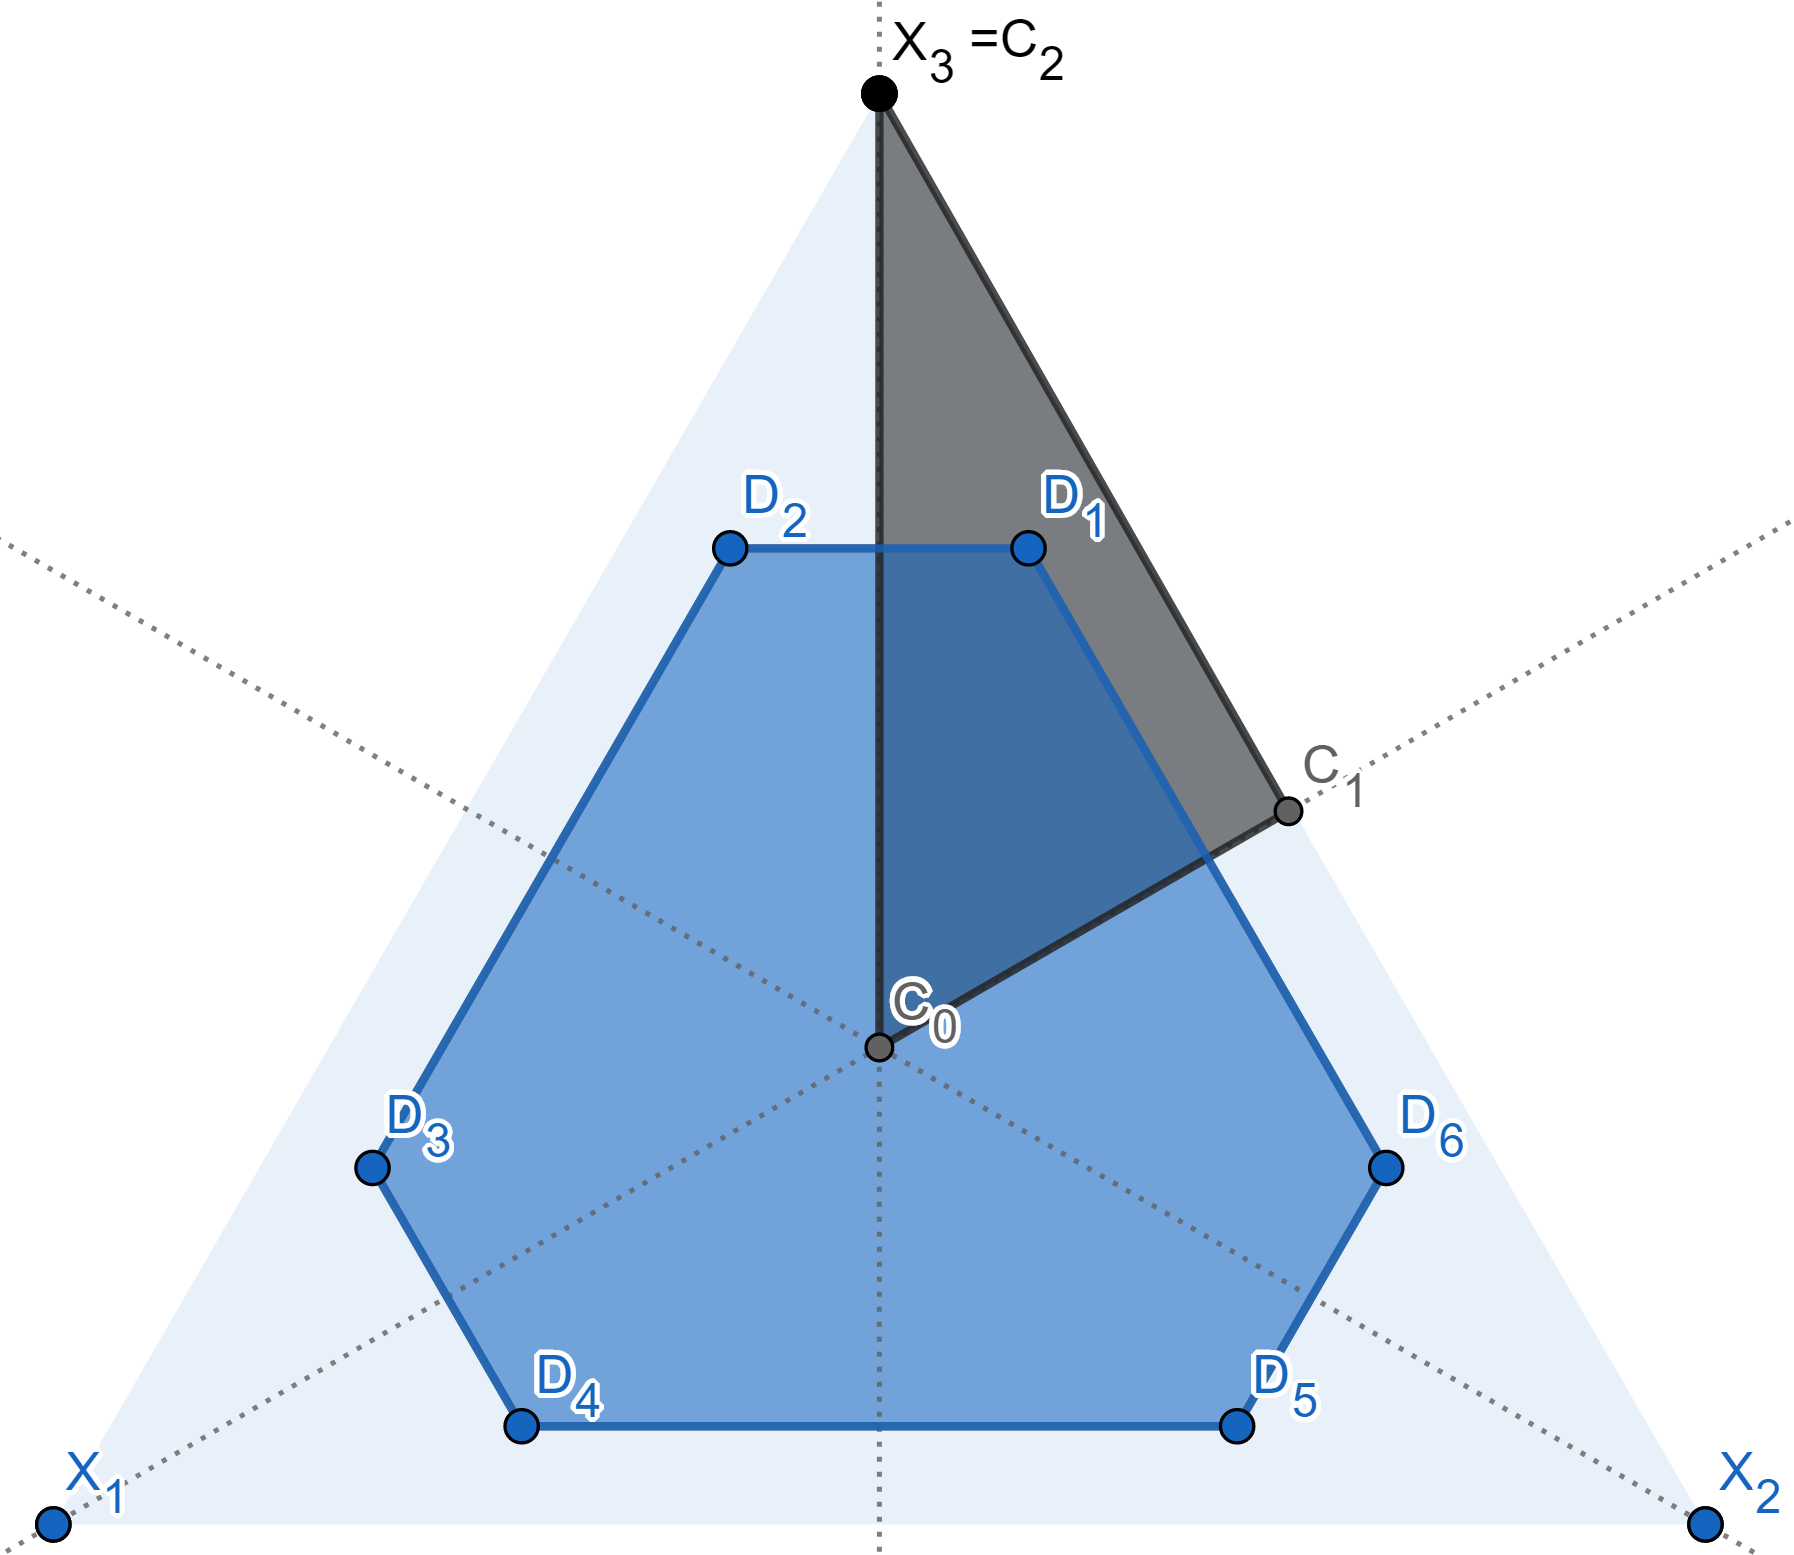
\includegraphics[width=0.7\textwidth]{fundamental_domain}
	\caption{The triangle \(\mathscr{D}\), when \(n=3\). Its three reflection symmetry axes are marked by dashed lines. Its three vertices are \(X_1 = (3,0,0), X_2 = (0,3,0), X_3=(0,0,3)\). Its center is \(C_0 = \mathds{1} = (1,1,1)\). Its fundamental domain is the dark triangle \(C_0C_1C_2\). The hexagon \(D_1D_2D_3D_4D_5D_6\) is generated by the point \(D_1\) in the fundamental domain.}
	\label{fig:fundamental_domain}
\end{figure}

\(\mathscr{D}_0\) can be regarded as a set of representatives from \(\mathscr{D}/\mathbb{G}\), and so, for any \(X\in \mathscr{D}\), there exists a unique element from its orbit that is in \(\mathscr{D}_0\). For any \(\mathscr{F}\subseteq \mathscr{D}\), if \(\mathscr{F}\) is invariant under the actions of \(\mathbb{G}\), that is, $\mathcal{F}$ is law invariant, then it is determined by \(\mathscr{F}\cap \mathscr{D}_0\), since it can be reconstructed by 
\[\mathscr{F} = \bigcup_{\pi \in \mathbb{G}} \left( \mathscr{F}\cap \mathscr{D}_0 \right) \circ \pi.\]

Let \(\Theta = \mathscr{F}\cap\mathscr{D}_0\). For each $p\in \Theta$, let $\mathscr{P}_p$ be the convex hull of $\mathbb{G}(p)$, which is shown in Figure \ref{fig:fundamental_domain} as a hexagon. Then it is geometrically clear that 
\begin{equation}
\mathscr{F} = \bigcup_{p\in \Theta} \mathscr{P}_p = \cl\co\bigcup_{p\in \Theta} \mathscr{P}_p.
\end{equation}
So by \cite[Table 3.3.1]{hiriart-urrutyFundamentalsConvexAnalysis2001}, since $\mathcal{F}$ is the support function of $\cup_{p\in\Theta}\mathscr{P}_p$, which is itself convex and closed, we have
\begin{equation}
\mathcal{F} = \sup_{p\in\Theta} \sigma_{\mathscr{P}_p}.
\end{equation}

Finally, since each $p\in\Theta$ is in $\mathscr{D}_0$, it is a convex sum of the vertices 
$$\left\{
C_0, C_1, ..., C_{n-1}
\right\} = \{q_0, q_1, ... q_{n-1} \}.$$
Thus, there exists a tuple $\theta_p = (\theta_{p, 0}, ..., \theta_{p, n-1})$, such that each $\theta_{p, i} \ge 0$, $\sum_{i = 0}^{n-1}\theta_{p, i} = 1$, and
$$
p = \sum_{i = 0}^{n-1}\theta_{p, i} C_i,
$$
which implies 
$$
\mathscr{P}_p = \co(\mathbb{G}(p)) = \sum_{i = 0}^{n-1}\theta_{p, i}\co(\mathbb{G}(q_i)),
$$
where the second equality is illustrated in Figure \ref{fig:triangle_symmetry}.

\begin{figure}[h]
	\centering
	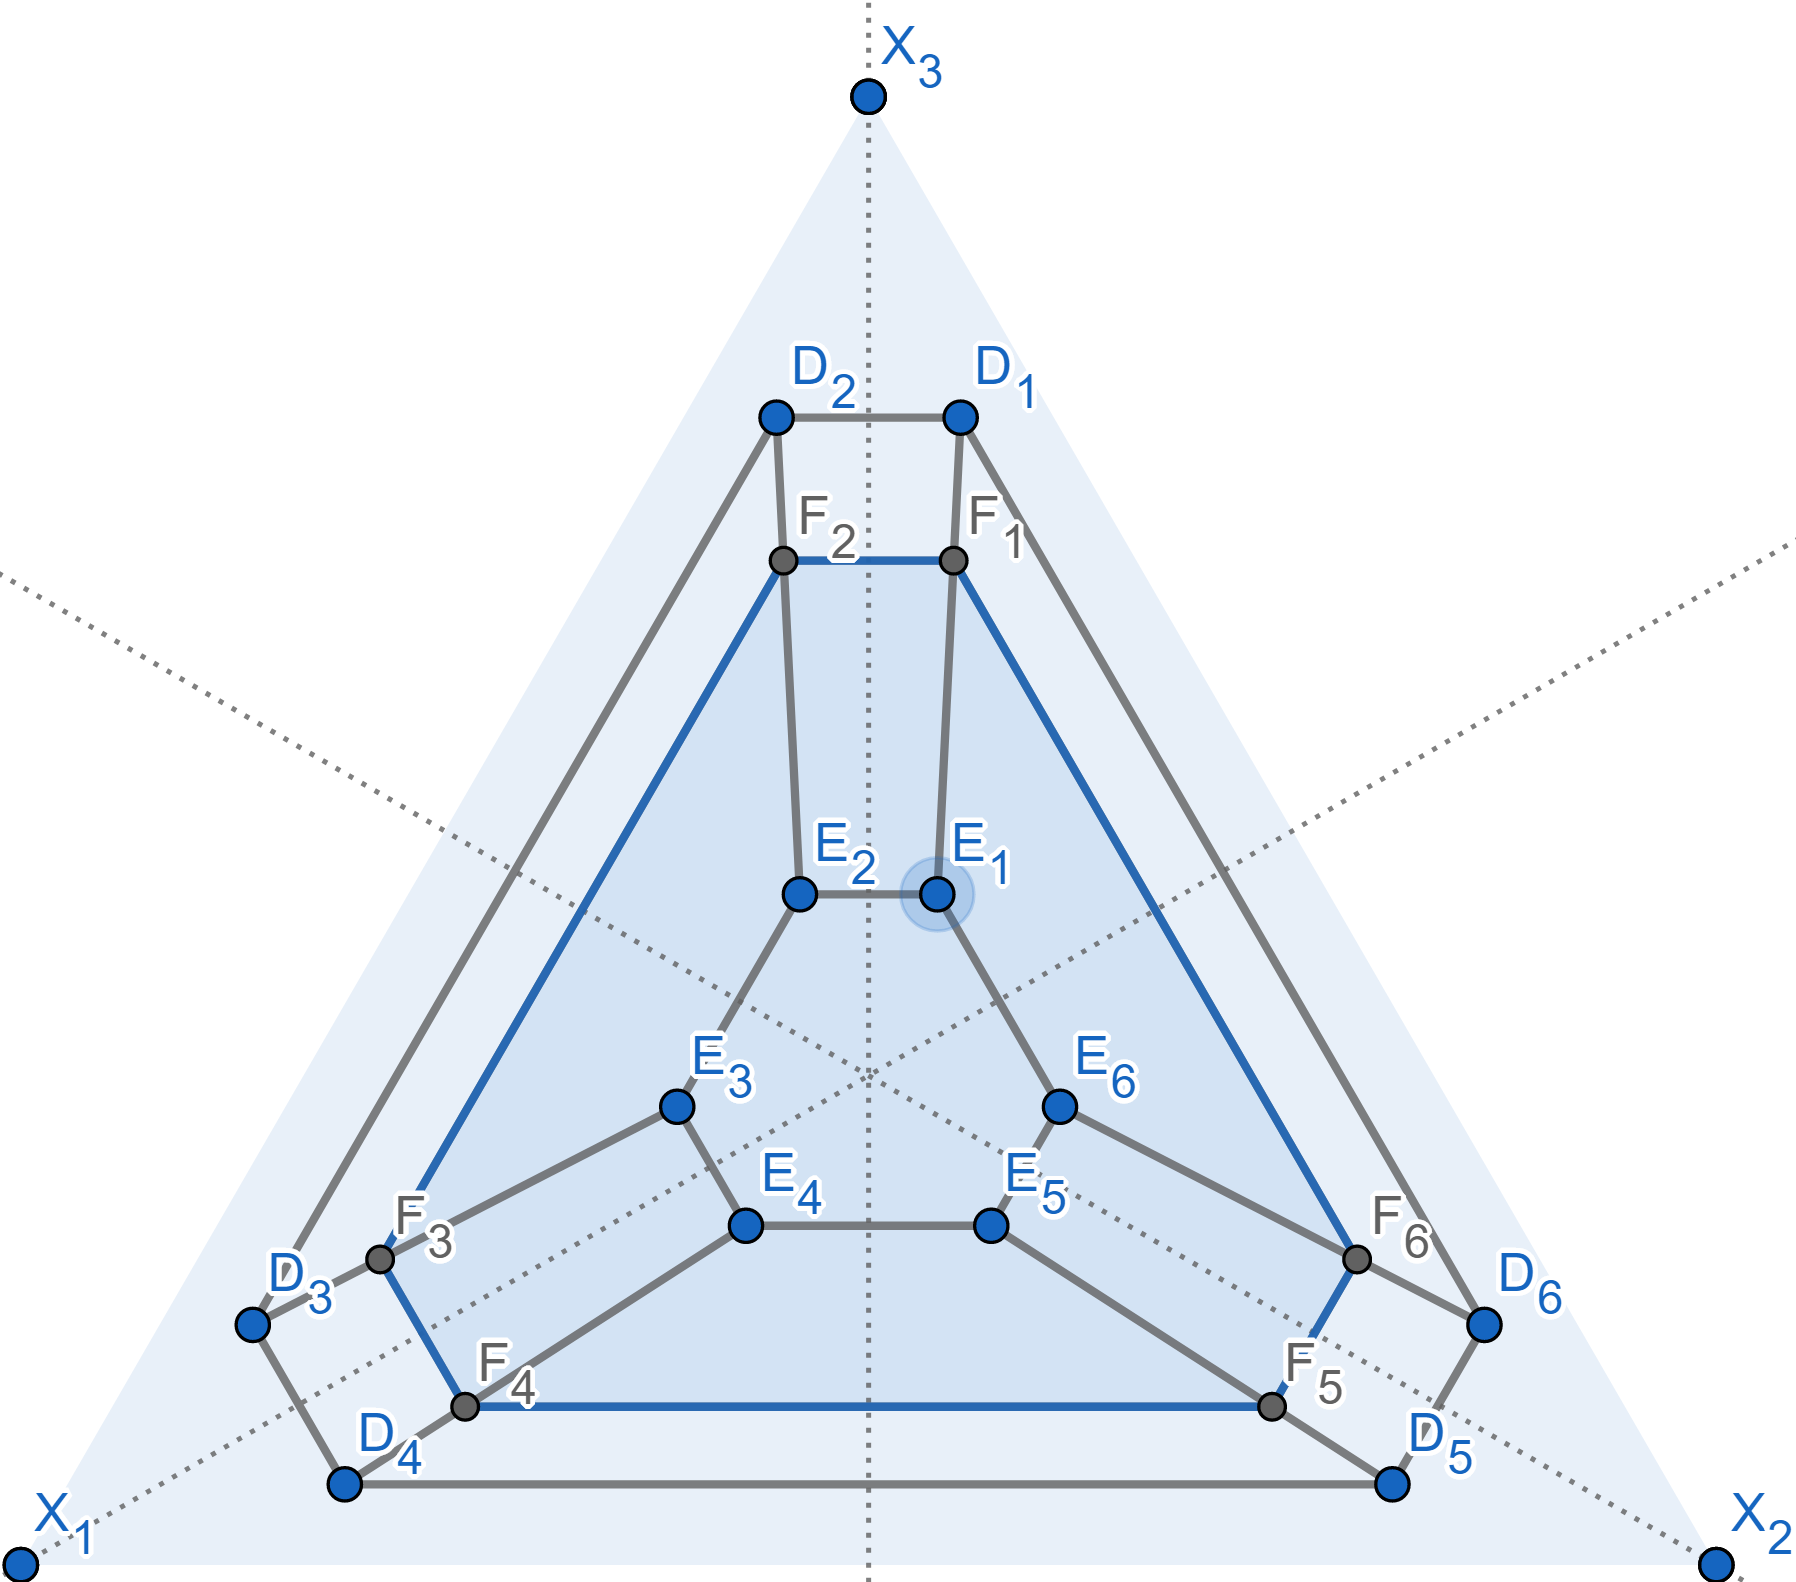
\includegraphics[width=0.6\textwidth]{triangle_symmetry}
	\caption{The triangle \(\mathscr{D}\), with three hexagons generated by the points \(D_1, E_1, F_1\) in the fundamental domain. \(F_1 = \theta D_1 + (1-\theta)E_1\). We have that \(\theta \mathbb{G}(D_1) + (1-\theta) \mathbb{G}(E_1) = \mathbb{G}(\theta D_1 + (1-\theta)E_1)\). In other words, the following two operations commute: interpolating between points in the fundamental domain, and generating a hexagon from a point in the fundamental domain.}
	\label{fig:triangle_symmetry}
\end{figure}

\begin{figure}[h]
	\centering
	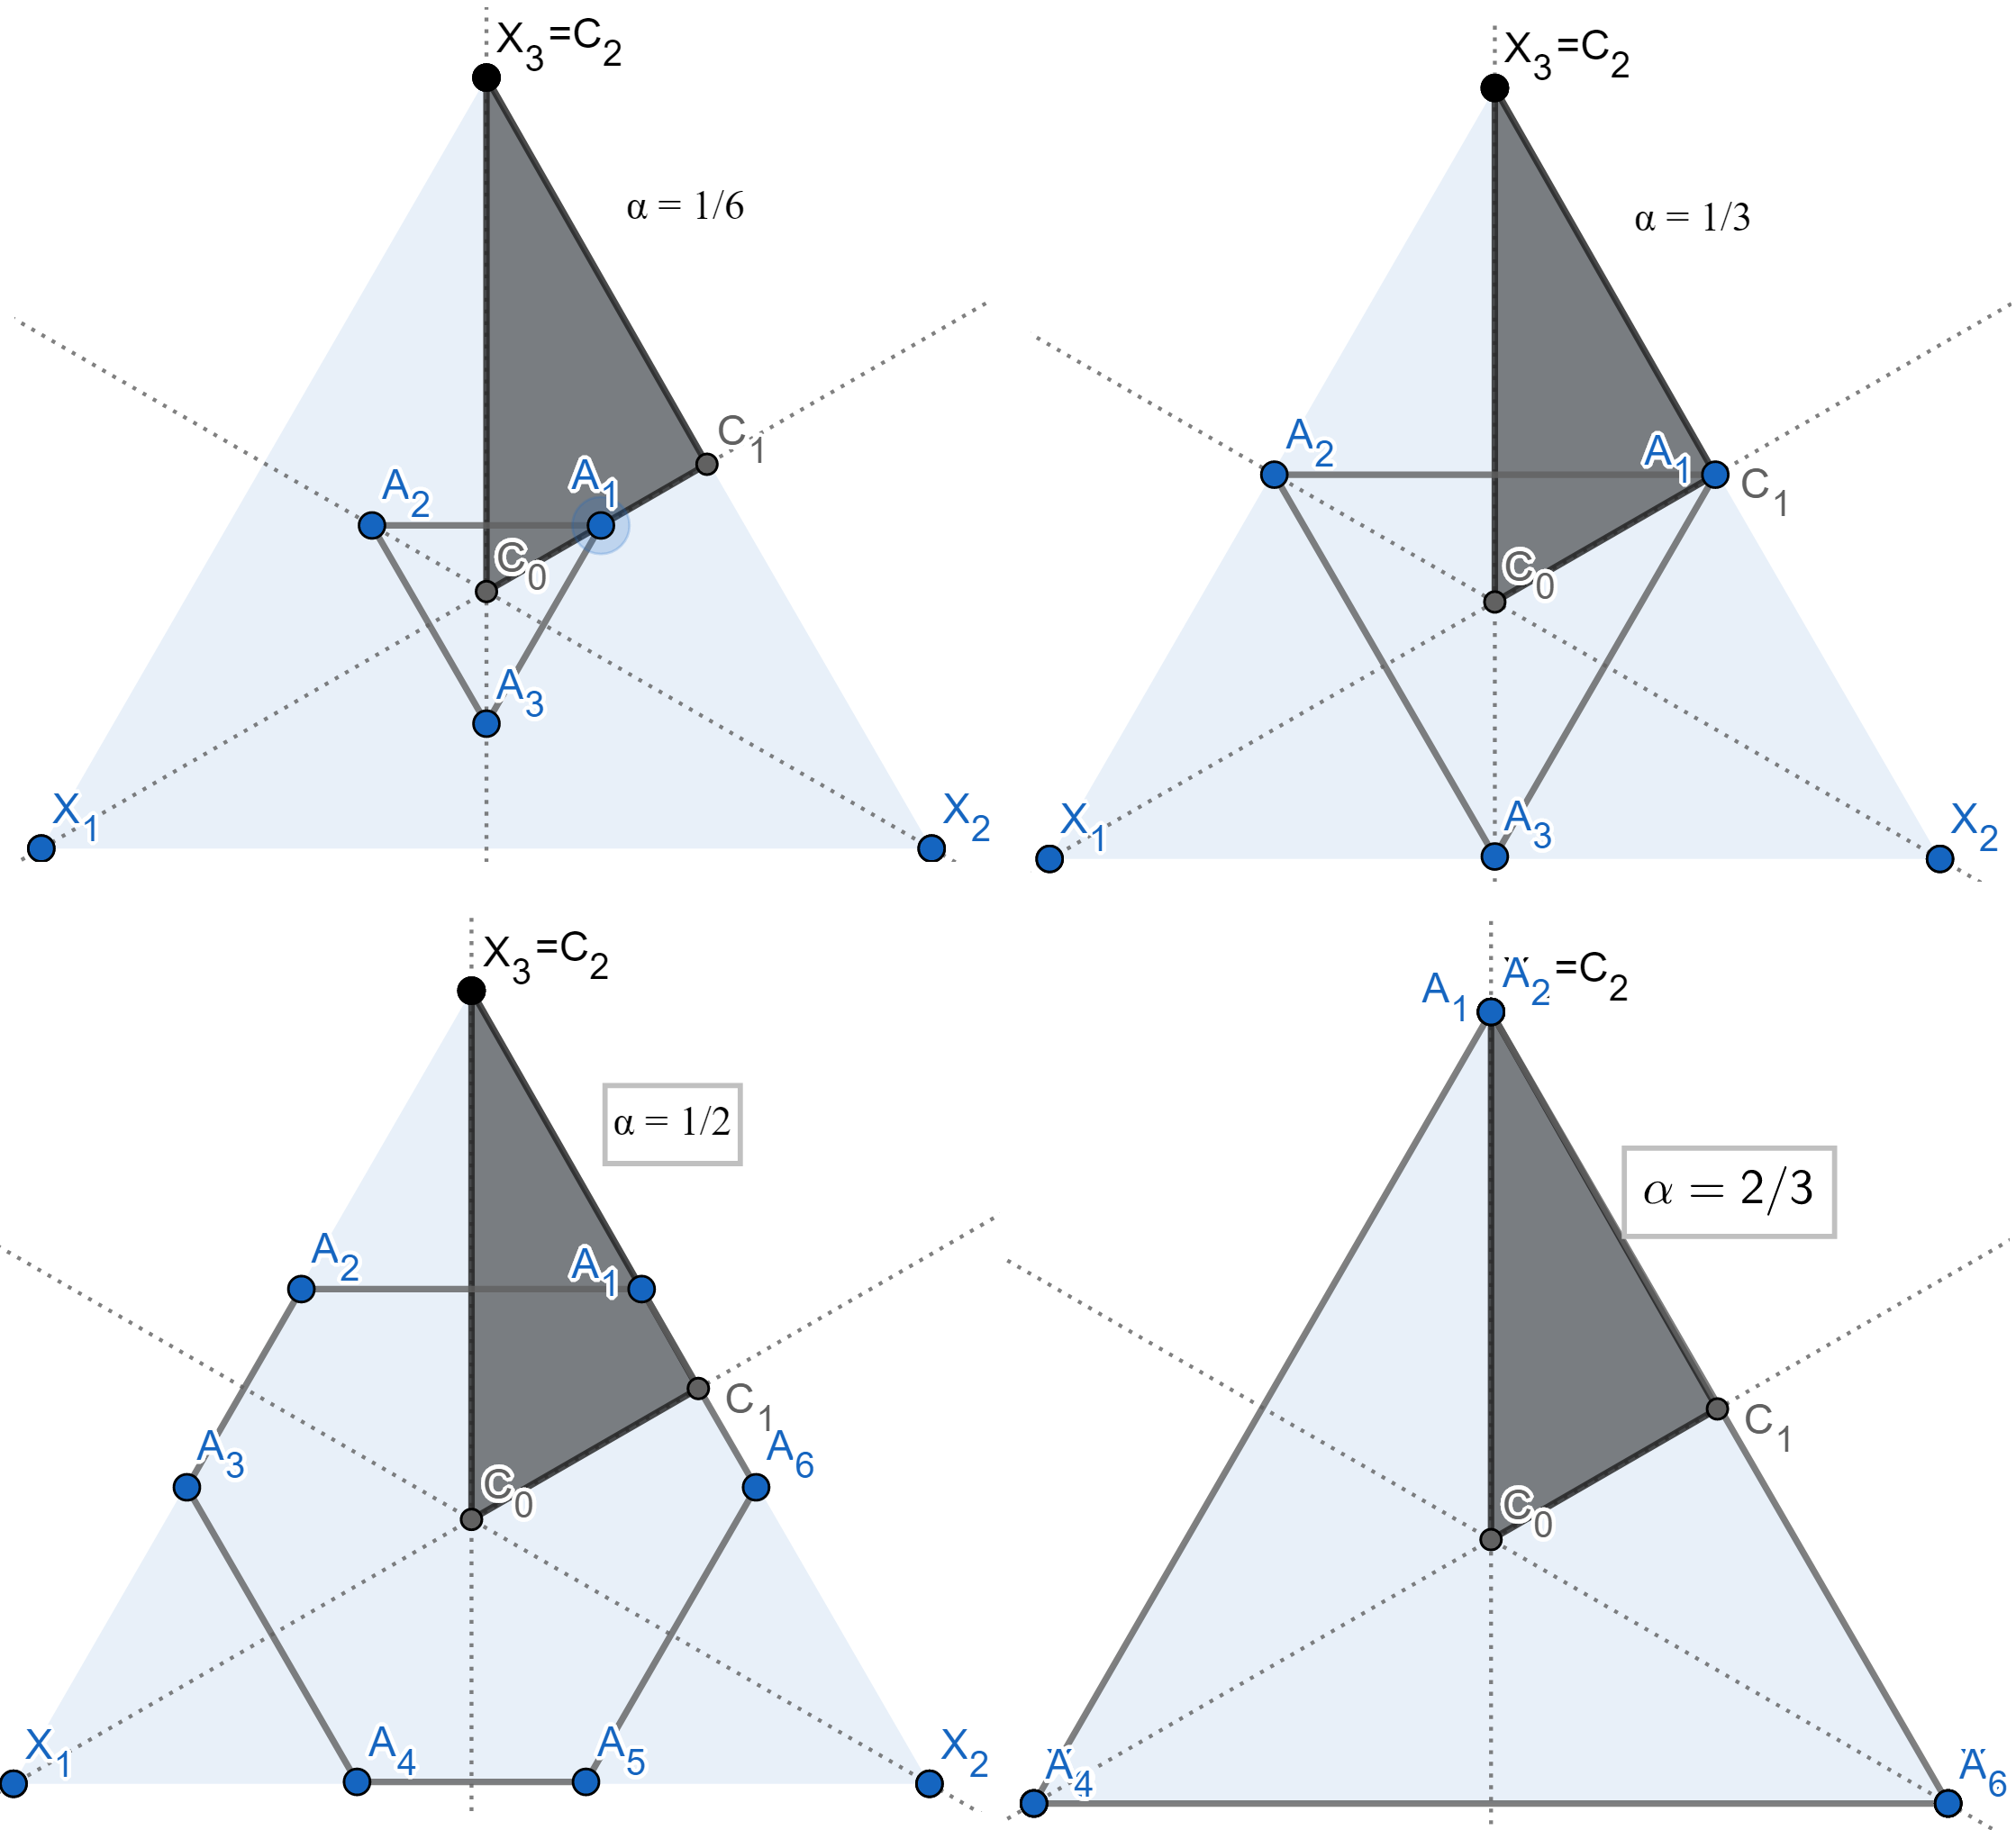
\includegraphics[width=0.7\textwidth]{growing_triangle_merged}
	\caption{\(\mathscr{C}_\alpha\) is generated by \(A_1\), which moves in the fundamental domain as \(\alpha\) increases. When \(\alpha\in [\frac{k}{n}, \frac{k+1}{n}]\), \(A_1\) is on the segment \(C_kC_{k+1}\).}
	\label{fig:growing_triangle_merged}
\end{figure}

Then, since $\co(\mathbb{G}(q_i)) = \mathscr{C}_{\frac i n}$, as illustrated in Figure \ref{fig:growing_triangle_merged}, we have
$$
\mathscr{F} = \bigcup_{p\in\Theta}\mathscr{P}_p = \bigcup_{p\in\Theta} \left(\sum_{i = 0}^{n-1}\theta_{p, i} \mathscr{C}_{\frac in} \right).
$$
Taking the support function on both sides, by \cite[Table 3.3.1]{hiriart-urrutyFundamentalsConvexAnalysis2001} again, 
$$
\mathcal{F} = \sup_{p\in\Theta} \sum_{i = 0}^{n-1}\theta_{p, i} \cvar_{\frac in}.
$$

We summarize the result in a proposition:

\begin{prop}
	If $S = [n]$, $ n \ge 2$, and $\nu$ is uniform on $S$, then any closed, sublinear, translation invariant, law invariant risk measure $\mathcal{F}$ is coherent. 
	
	Let its risk envelope be $\mathscr{F}$. Let $\mathscr{D}_0$ be a fundamental domain of $\mathscr{D}$, defined as in Equation \ref{eq:fundamental_domain}.
	 
	Define $\Theta = \mathscr{D}_0 \cap \partial \mathscr{F}$, then for each $p \in \Theta$, let $\mathscr{P}_p$ be the convex hull of $\mathbb{G}(p)$, then there exists a tuple $\theta_p = (\theta_{p, 0}, ..., \theta_{p, n-1})$, such that each $\theta_{p, i} \ge 0$, $\sum_{i = 0}^{n-1}\theta_{p, i} = 1$, and
	\begin{equation}
	\mathscr{P}_p = \sum_{i = 0}^{n-1}\theta_{p, i} \mathscr{C}_{\frac in},
	\end{equation}
	and we have the Kusuoka representation 
	\begin{equation}
	\mathcal{F} = \sup_{p\in\Theta} \sum_{i = 0}^{n-1}\theta_{p, i} \cvar_{\frac in}.
	\end{equation}
\end{prop}

\subsection{The case of nonuniform probability on \(S\)}
\label{sec:nonuniform_space}
Let \(S = [n]= \{1, 2, \cdots , n\} \), where \(n \) is an integer at least \(2\). Let \(\nu\) be a nonuniform probability measure on \(S\). 

For this section, we do a specific example, which is a sufficiently illustrative example for the general \(n \ge 2\) cases.

Let \(n=4\); let \(\nu \) be defined by
\[\nu: 1\mapsto \frac{1}{6}, 2\mapsto \frac{1}{6}, 3\mapsto \frac{1}{3}, 4\mapsto \frac{1}{3}\]
Thus, its symmetry group \(\mathbb{G}\) has \(4\) elements, and breaks \(S\) into two orbits: \(\{1, 2\} \) and \(\{3,4\} \). 

Let the centroids of the orbits be \(A = \frac{X_1 + X_2}{2}, B = \frac{X_3 + X_4}{2}\), and let \(C = \mathds{1}\).

Take any closed convex \(\mathscr{F} \subseteq \mathscr{D}\) that contains \(C\) in its interior (relative to \(\mathscr{D}\)). Connect \(A, B\), making a line passing \(C\) and intersecting \(\partial\mathscr{F}\) at two points $D, E$. This is shown in Figure \ref{fig:tetrahedron_homothety}.

Define the \textbf{line ratio} of \(\mathscr{F}\) be 
$$LR(\mathscr{F}) = \overline{DC} : \overline{CE},$$
and let $r_0 = LR(\mathscr{D}) = \overline{AC} : \overline{CB}$. Without loss of generality, assume that $\overline{AC} \ge \overline{CB}$, so that $r_0 \ge 1$. 

In our particular example, it happens that $\overline{AC} = \sqrt{10}, \overline{CB} = \sqrt{10}/2$, so $r_0 = 2$.

For small $\alpha > 0$, $\mathscr{C}_\alpha$ is an inverted homothetic image of $\mathscr{D}$, so $LR(\mathscr{C}_\alpha) = 1/r_0$. For big $\alpha < 1$, we have $D = A$ and $E = B$, so $LR(\mathscr{C}_\alpha) = r_0$. Between them, we have 
$$\forall \alpha\in (0, 1], LR(\mathscr{C}_\alpha)\in [1/r_0, r_0].$$
This is in fact true in general for all Kusuoka-representable sets:

\begin{prop}[Kusuoka set line ratio]
Take any nontrivial Kusuoka set, as defined in Equation \ref{eq:kusuoka_set}:
$$
\mathscr{F} = \cl\co\bigcup_{\theta \in \Theta}\int_0^1 \mathscr{C}_\alpha dm_\theta(\alpha),
$$
and assume it is nontrivial, that is, $\mathscr{F}\neq \{\mathds{1}\}$. Then $LR(\mathscr{F}) \in [1/r_0, r_0]$.
\end{prop}
\begin{proof}\textit{(Sketch)} Refer to Figure \ref{fig:tetrahedron_homothety}.

	Translate the origin of the coordinate frame to point $C$. So, for example, $A$ in the new coordinate frame is $(2,2,-1,-1)$.
	
	For each point $P\in\mathbb{R}^n$, let $f(P)$ be its projection onto the line $AB$, and define $d(P)$ to be the directed distance from $C$ to $f(P)$. So, for example, $d(A) = \sqrt{10}, d(B) = -\sqrt{10}/2$.
	
	Since the affine subspaces spanned by $\{X_1, X_2\}$ and spanned by $\{X_3, X_4\}$ are perpendicular to line $AB$, the projection of $\mathscr{D}$ onto the line $AB$ is the line segment $[A,B]$.
	
	Then, for any $\alpha \in (0, 1]$, 
	$$f(\mathscr{C}_\alpha) = [D_\alpha, E_\alpha] = AB \cap \mathscr{C}_\alpha,$$
	where we append the subscript $\alpha$ to $D, E$ to denote its association with $\mathscr{C}_\alpha$. Then the line ratio of $\mathscr{C}_\alpha$ is 
	$$LR(\mathscr{C}_\alpha) = -\frac{d(D_\alpha)}{d(E_\alpha)}\in[1/r_0, r_0]$$
	
	For any probability measure $m_\theta$ on $[0, 1]$, let $\mathscr{P}_\theta = \int_0^1 \mathscr{C}_\alpha dm_\theta(\alpha)$. Then $f(\mathscr{P}_\theta) = [D_\theta, E_\theta]$, where 
	$$d(D_\theta) = \int_0^1 d(D_\alpha) dm_\theta(\alpha), \quad d(E_\theta) = \int_0^1 d(E_\alpha) dm_\theta(\alpha).$$
	Thus, 
	$$LR(\mathscr{P}_\theta) = -\frac{d(D_\theta)}{d(E_\theta)}\in[1/r_0, r_0].$$
	
	Finally, let $\mathscr{F} = \cl\co\bigcup_{\theta \in \Theta}\mathscr{P}_\theta$, we have
	$$d(\mathscr{F}) = \left[\inf_{\theta \in \Theta} d(E_\theta), \sup_{\theta \in \Theta} d(D_\theta)\right],$$
	and so
	$$LR(\mathscr{F}) \in [1/r_0, r_0].$$
\end{proof}


\begin{figure}[h]
	\centering
	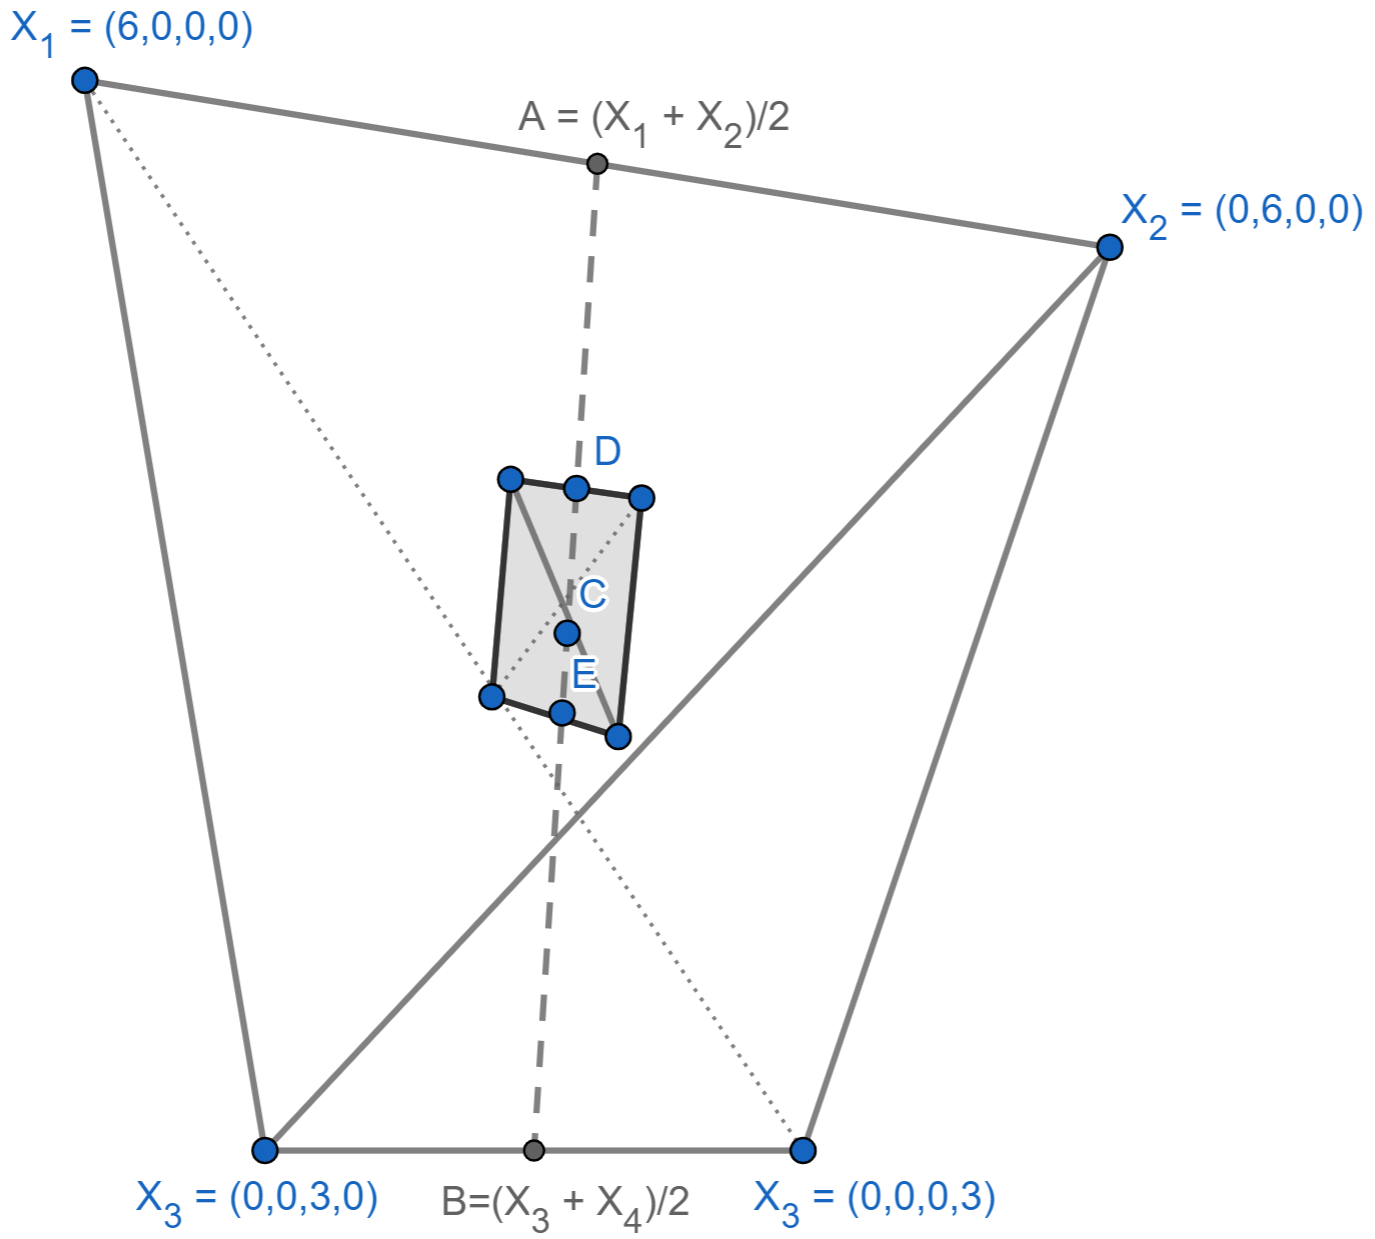
\includegraphics[width=0.7\textwidth]{tetrahedron_homothety}
	\caption{When \(n = 4\), \(\mathscr{D}\) is a tetrahedron, centered at \(C = \mathds{1} = (1,1,1,1)\). With the \(\nu\) defined in the text, the tetrahedron is not regular. For a small \(\alpha\), \(\mathscr{C}_\alpha\) is a small homothetic copy of \(\mathscr{D}\), here drawn in the center in gray. The "line ratio" is obtained by connecting \((X_1 + X_2)/2\) and \((X_3 + X_4)/2\), cutting \(\mathscr{C}_\alpha\) at \(D, E\), then defining the ratio as \(\overline{DC} : \overline{CE}\).}
	\label{fig:tetrahedron_homothety}
\end{figure}

\begin{figure}[h]
	\centering
	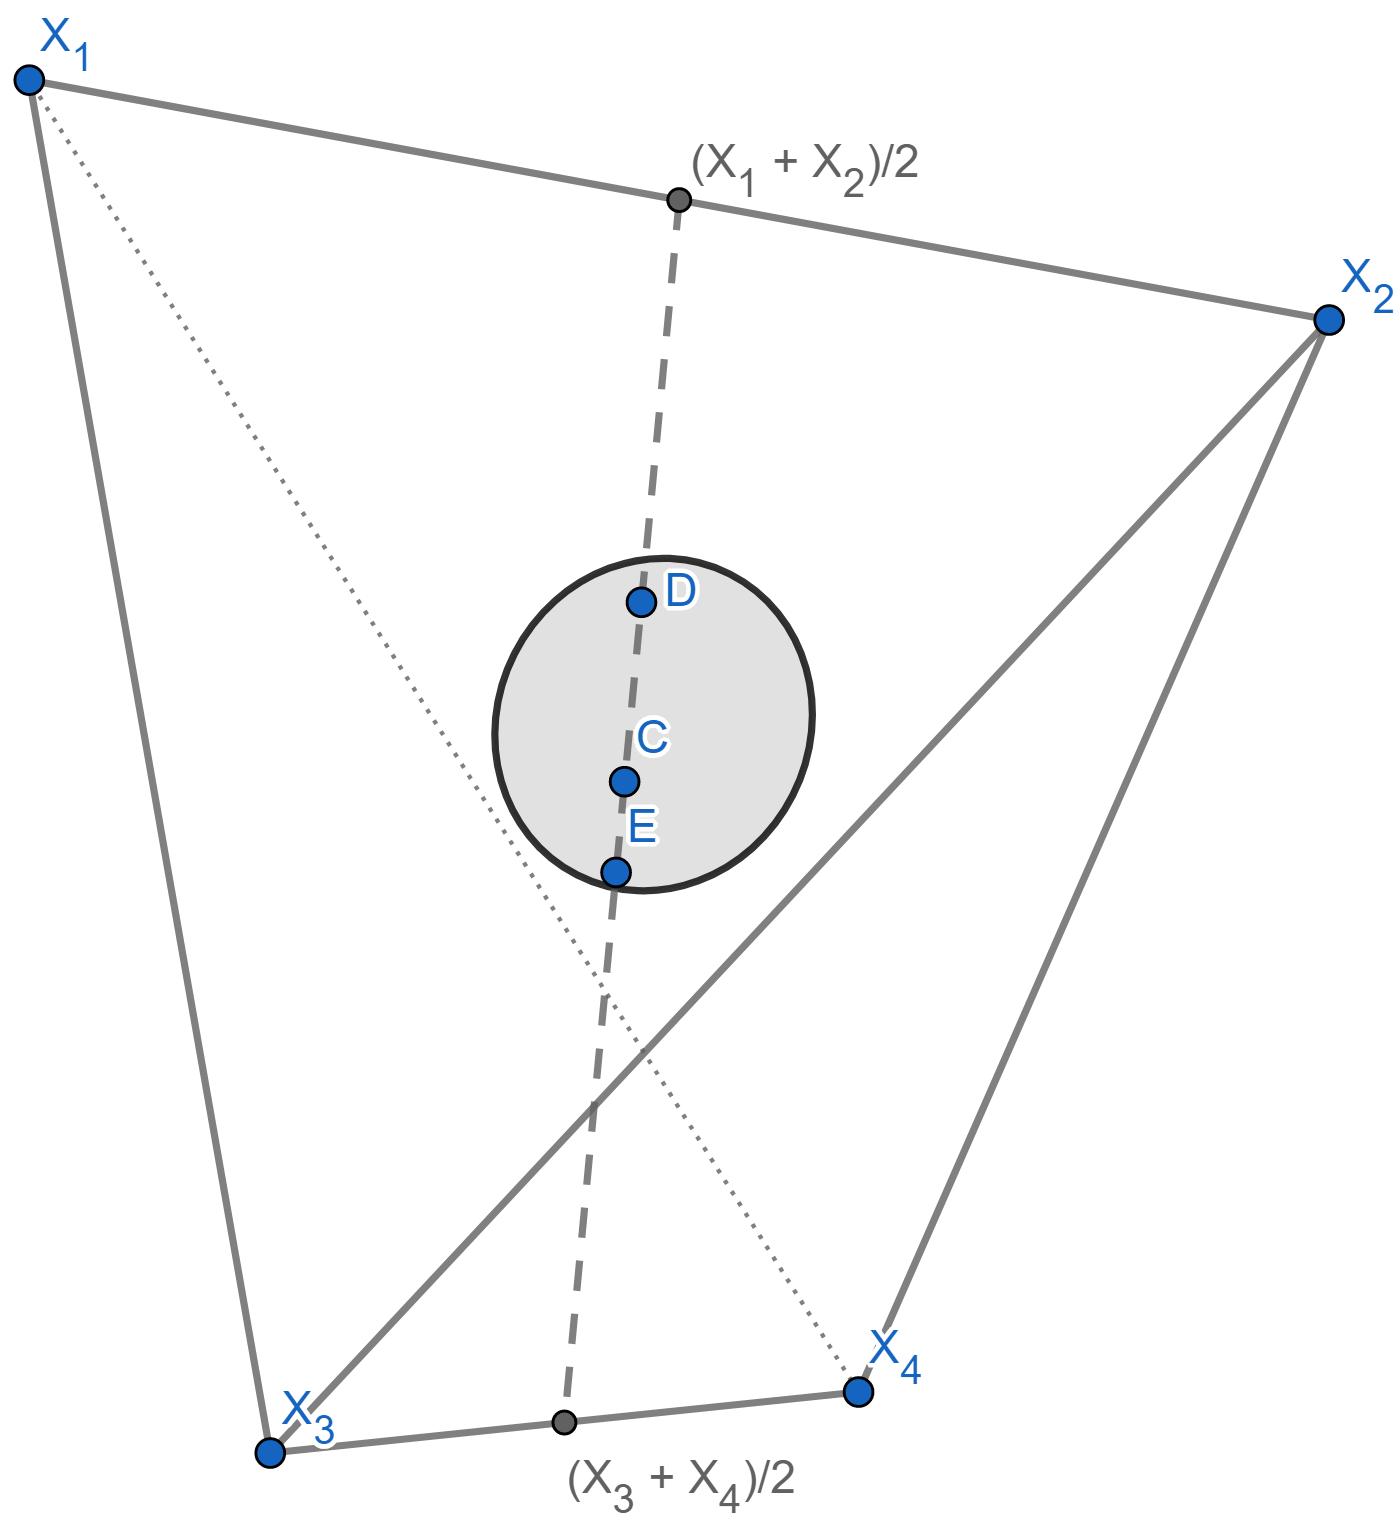
\includegraphics[width=0.5\textwidth]{tetrahedron_irregular}
	\caption{To construct a closed, law invariant, strictly risk averse, coherent risk measure that has no Kusuoka representation, take a small closed ball around \(\mathds{1}\), then shift it along the line connecting \((X_1 + X_2)/2\), \((X_3 + X_4)/2\), until its line ratio moves out of the bound.}
	\label{fig:tetrahedron_irregular}
\end{figure}

To violate this line ratio, simply take a closed ball of very small radius \(r\), in \(\mathscr{D}\) around \(\mathds{1}\), then shift it by \((1-\epsilon)r\) in the direction of \(\frac{X_1 + X_2}{2} - \frac{X_3 + X_4}{2}\). Let the resulting set be \(\mathscr{F}\), then \(\mathcal{F} = \sigma_{\mathscr{F}}\) is a closed, law invariant, strictly risk averse, coherent risk measure that can be arbitrarily close to \(\mathbb{E}\), and yet has no Kusuoka representation.

Also, note that if we shift the ball by \((1 + \epsilon)r\) instead, then we obtain a closed, law invariant, coherent risk measure that is not risk averse, and can be arbitrarily close to \(\mathbb{E}\). This contrasts with the case of uniform probability on \(S\), where any law invariant, coherent risk measure is either \(\mathbb{E}\) or strictly risk-averse.

We record this formally as:

\begin{prop}
	If $S = [n]$, $ n \ge 2$, and $\nu$ is nonuniform on $S$, then there exists closed, law invariant, risk averse, coherent risk measures that are arbitrarily close to $\mathbb{E}$, and yet have no Kusuoka representations.
\end{prop}


  
\chapter{Inequalities of coherent risk measures}
\label{chapter_inequalities}

Inequalities are the foundation of any analytical treatment of a subject. Here, we collect and prove many inequalities for coherent risk measures. Most of them are generalizations to inequalities that involve expectation.

We cannot find in the literature the inequalities that follow, so we believe these are new results. However, in \cite[Chapter 3]{zabarankinStatisticalDecisionProblems2016}, the authors presented similar probability inequalities for general risk measures.

\section{Elementary inequalities}\label{sec:elementary_inequalities}
\begin{prop}[Cauchy--Schwarz inequality]
For any sublinear, monotonic functional $\mathcal{F}$ on $\mathscr{L}^2$, and any $X, Y\in \mathscr{L}^2$, if $\mathcal{F}(XY) \le 0$, then 
\begin{equation}
\label{eq:csineq_crm}
\mathcal{F}(XY)^2 \le \mathcal{F}(X^2)\mathcal{F}(Y^2)
\end{equation}
Similarly, if $\mathcal{F}(-XY)\le 0$, then 
\begin{equation}
\label{eq:csineq_crm_2}
\mathcal{F}(-XY)^2 \le \mathcal{F}(X^2)\mathcal{F}(Y^2)
\end{equation}
\end{prop}
\begin{proof}
For the first case, let $\lambda =\mathcal{F}(XY)/\mathcal{F}(Y^2)$, and expand the right side of 
$$0\le \mathcal{F}((X-\lambda Y)^2)$$. 

The second case is converted to the first case by changing the sign of $X$.
\end{proof}

Jensen's inequality does not generalize easily. \cite[Theorem 3]{chenRiskMeasuresNonlinear2013} shows that any coherent risk measures that is a $g$-expectation obeys Jensen's inequality, but since we have no use for $g$-expectation in this thesis, this result will be skipped.

Two inequalities for expectations extend trivially via the dual representation of coherent risk measures (Proposition \ref{prop:dual_crm}).
\begin{prop}[H\"older inequality]
	For any closed, coherent risk measure $\mathcal{F}$ on $\mathscr{L}^2$, and any $p, q > 0$ such that $\frac 1 p + \frac 1 q = 1$, for any $X, Y\in \mathscr{L}^2$ with finite $\mathbb{E}(|X|^p), \mathbb{E}(|Y|^q)$, then 
	\begin{equation}
		\mathcal{F}(|XY|) \le \mathcal{F}(|X|^p)^{1/p} \mathcal{F}(|Y|^q)^{1/q}.
	\end{equation}
\end{prop}
\begin{proof}
	As in Equation \ref{eq:dual_crm}, take the dual representation of $\mathcal{F}$:
	$$\mathcal{F}(Z) = \sup_{\theta\in\Theta} \mathbb{E}_\theta(Z)$$
	Then
	\begin{align*}
		\mathcal{F}(|XY|) &= \sup_{\theta\in\Theta} \mathbb{E}_\theta(|XY|) \\
			&\le \sup_{\theta\in\Theta}\left( \mathbb{E}_\theta(|X|^p)^{1/p} \mathbb{E}_\theta(|Y|^q)^{1/q}\right) 
			\quad\text{ (H\"older inequality)}\\
			&\le \left(\sup_{\theta\in\Theta} \mathbb{E}_\theta(|X|^p)^{1/p}\right)
			\left(\sup_{\theta\in\Theta} \mathbb{E}_\theta(|Y|^q)^{1/q}\right)\\
			&= \left(\sup_{\theta\in\Theta} \mathbb{E}_\theta(|X|^p)\right)^{1/p}
			\left(\sup_{\theta\in\Theta} \mathbb{E}_\theta(|Y|^q)\right)^{1/q}\\
			&= \mathcal{F}(|X|^p)^{1/p}\mathcal{F}(|Y|^q)^{1/q}.
	\end{align*}
\end{proof}

\begin{prop}[Minkowski inequality]
	Under the same assumptions as above,
	\begin{equation}
	\mathcal{F}(|XY|) \le \mathcal{F}(|X|^p)^{1/p} + \mathcal{F}(|Y|^q)^{1/q}.
	\end{equation}
\end{prop}
\begin{proof}
	Essentially the same as the previous proof.
\end{proof}

\section{Concentration inequalities}\label{sec:tail_ineq}
A "nice" random variable should be "far" to its expectation with a small probability, that is, its value should be concentrated around its expectation. Concentration inequalities quantify this vague statement in various ways.

In this section, we prove generalizations of Markov, Chebyshev, Chernoff, Hoeffding, Bennett, and Bernstein's inequalities. These inequalities are the most important tail inequalities, heavily used in all parts of statistics, probability, and machine learning. As one example, the Hoeffding inequality is the basis of the popular Monte Carlo tree search algorithm UCT\cite{kocsisBanditBasedMonteCarlo2006}.

\begin{prop}[Markov's inequality]\label{prop:markov}
Given any monotonically increasing $\phi : [0, \infty) \to [0, \infty)$, any $a \ge 0, X\in\mathscr{L}$, and monotonic, positively homogenous functional $\mathcal{F}$,
\begin{equation}
\label{eq:markov}
\mathcal{F}(\phi(|X|)) \ge \phi(a) \mathcal{F}(1_{|X|\ge a})
\end{equation}

Similarly, if $\phi: \mathbb{R} \to [0, \infty)$ is monotonically increasing, then for any $a$, 
\begin{equation}
\label{eq:markov_2}
\mathcal{F}(\phi(X)) \ge \phi(a) \mathcal{F}(1_{X\ge a})
\end{equation} 
\end{prop}
\begin{proof}
For the first case, since $\phi(|X|) \ge \phi(a) 1_{|X|\ge a}$, by monotonicity of $\phi$ and positive homogeneity of $\mathcal{F}$, 
$$\mathcal{F}(\phi(|X|)) \ge  \mathcal{F}(\phi(a)1_{|X|\ge a}) = \phi(a)\mathcal{F}(1_{|X|\ge a}). $$

Similarly for the second case.
\end{proof}

\begin{prop}[Chebyshev's inequality]
Given any $a > 0, X\in\mathscr{L}$, and monotonic, positively homogenous functional $\mathcal{F}$,
\begin{equation}
\label{eq:chebyshev}
\mathcal{F}(1_{|X|\ge a})\le \frac{1}{a^2}\mathcal{F}(X^2) 
\end{equation}
\end{prop}
\begin{proof}
Let $\phi(a) = a^2$ in the first Markov's inequality.
\end{proof}

\begin{prop}[Chernoff bound]
Given any $t > 0, X\in\mathscr{L}$, and monotonic, positively homogenous functional $\mathcal{F}$,
\begin{equation}
\label{eq:chernoff}
\ln\mathcal{F}(1_{X\ge t}) \le -\sup_{a \ge 0}(ta - \ln\mathcal{F}(e^{aX}))
\end{equation}
\end{prop}
\begin{proof}
Let $\phi(x) = e^{tx}$ in the second Markov's inequality, to get 
$$\mathcal{F}(1_{X\ge t}) \le e^{-ta}\mathcal{F}(e^{tX})\quad \text{for any } a > 0.$$

Then take logarithm on both sides, and take the infimum over $a > 0$ on the right side. 

Note that the $a = 0$ case gives $\ln\mathcal{F}(1_{X\ge t}) \le 0$, which is trivially true, since 
$$\mathcal{F}(1_{X\ge t}) \le \mathcal{F}(1) = 1,$$
so it can be incorporated safely into the infimum.
\end{proof}

We record a particularly useful case for \cvar:

\begin{cor}[Chernoff bound for \cvar]
	\label{thm:chernoff_cvar}
	Given any real random variable $X$ with finite first moment, any $\alpha \in [0, 1]$, and any $a > \var_\alpha(X)$, we have 
	\begin{equation}
	\label{eq:chernoff_cvar}
		Pr(X \ge a) \le {\overbar{\alpha}} \inf_{t > 0} \cvar_\alpha(e^{tX}) e^{-ta}
	\end{equation}
\end{cor}
\begin{proof}
	In Chebyshev's inequality, replace $\mathcal{F}, a, X$ by $\cvar_\alpha, 1, e^{t(X - a)/2}$, to obtain
	$$\cvar_\alpha(1_{X \ge a}) = \cvar_\alpha(1_{e^{t(X-a)/2} \ge 1}) \le \cvar_\alpha(e^{t(X-a)}) = \cvar_\alpha(e^{tX}) e^{-ta}$$
	for any $ t> 0$.
	
	Since $a > \var_\alpha(X)$, we have $Pr(X \ge a) \le {\overbar{\alpha}}$, and so
	$$\cvar_\alpha(1_{X \ge a}) = \min(1, Pr(X \ge a)/{\overbar{\alpha}}) = Pr(X \ge a)/{\overbar{\alpha}}.$$
	Optimize over $t$ to obtain the result.
\end{proof}

\begin{prop}[Hoeffding's lemma]
For any coherent risk measure $\mathcal{F}$ on $\mathscr{L}$, and $X$ such that $Pr(a\le X \le b) = 1$, let 
$$c(t) = \frac{\mathcal{F}(X) + \mathcal{F}(-X)}{e^{t(b-a)} - 1},$$
then for any $t\in\mathbb{R}, t\neq 0$,
\begin{equation}
\label{eq:hoeffding_lemma}
\mathcal{F}(\exp{[t(X - \mathcal{F}(X) - c(t))]}) \le \exp\left(\frac 1 8 (b-a)^2 t^2\right)
\end{equation}
\end{prop}
\begin{proof}
Rewrite $X$ as a convex sum of $a, b$:
$$X = \theta b + (1-\theta) a.$$
By convexity of $x\mapsto e^{tx}$, 
$$e^{tX} \le \theta e^{tb} + (1-\theta)e^{ta} = \frac{1}{b-a}((X-a)e^{tb} + (b-X)e^{ta})$$
Then by the coherence of $\mathcal{F}$, 
$$\mathcal{F}(e^{tX}) \le \frac{e^{tb}}{b-a}(\mathcal{F}(X) -a ) + \frac{e^{ta}}{b-a}(\mathcal{F}(-X) + b)$$

Replace $X$ by $X - \mathcal{F}(X) - c(t)$ in the above equation, and simplify, using translation invariance of $\mathcal{F}$, to cancel out the $\mathcal{F}$ terms on the right. This yields
\begin{align*}
\mathcal{F}(\exp{[t(X - \mathcal{F}(X) - c(t))]}) &\le \frac{be^{ta}-a e^{tb}}{b-a} = e^{g(u)}
\end{align*}
where 
$$
\begin{cases}
u = t(b-a)\\
g(u) = -\gamma u + \ln(1-\gamma + e^u \gamma)\\
\gamma = -\frac{a}{b-a}
\end{cases}
$$
Since $$
\begin{cases}
g(0) = 0\\
g'(0) = 0\\
g''(u) \le \frac 1 4 \quad \text{for } u\ge 0
\end{cases}
$$
we have
$$g(u) \le \frac 1 8 u^2 = \frac 1 8 t^2(b-a)^2$$
yielding the result.
\end{proof}

Hoeffding's lemma is often used to prove Hoeffding's inequality. However, the proof does not generalize immediately to general CRM, or even \cvar, because it depends on that for any two independent $X, Y\in \LL^1$, $\E(XY) \le \E(X)\E(Y)$, which is false for $\cvar$ in general:

\begin{ex}
	Given independent $X, Y$, it is not the case that $\mathcal{F}(XY) = \mathcal{F}(X) \mathcal{F}(Y)$. In fact, even for $\cvar_\alpha$, it is possible for one side to be arbitrarily greater than the other.
	
	Let $X, Y$ both have the distribution on $\{-T, T\}$ defined by 
	$$Pr(X = -T) = \frac 3 4, \quad Pr(X = T) = \frac 1 4$$ 
	$T$ being a positive constant, then 
	$$\cvar_{1/2}(X) = \cvar_{1/2}(Y) = 0 $$
	$$\cvar_{1/2}(XY) = T^2$$
	so $\cvar_{1/2}(XY)$ can be arbitrarily greater than $\cvar_{1/2}(X)\cvar_{1/2}(Y)$.
\end{ex}

However, when $X, Y\ge 0$ almost surely, we do have:
\begin{prop}
	For any two independent $X, Y\in \LL^1$ that are almost surely non-negative, and any $\alpha \in [0, 1]$, 
	\begin{equation}
		\cvar_\alpha(XY) \le \cvar_\alpha(X)\cvar_\alpha(Y).
	\end{equation}
\end{prop}
\begin{proof}	
	By continuity of $\cvar_\alpha$ with respect to $\alpha$, it suffices to prove this for all rational $\alpha \in(0, 1)$. 
	
	By closedness of $\cvar_\alpha$, it suffices to prove this for all $X, Y$ in a dense subset of $\LL^1$.
	
	For any $\alpha = \frac m n$, with $0< m < n$ integers, we prove this proposition for the dense subset of $\LL^1$:
	$$ \left\{X\in \LL^1 : X \text{ has distribution } \frac 1{N} \sum_{i= 1}^{N} \delta_{x_i}, n\text{ divides }N, \text{ and all } x_i \ge 0 \right\}.$$
	This subset is chosen, because it makes $\cvar_\alpha(X)$ easy to calculate: 
	$$\cvar_\alpha(X) = \frac 1{{\overbar{\alpha}} N}\sum\left(\text{the biggest } {\overbar{\alpha}} N \text{ terms of }x_i\right)$$
	for any such $X$. That is, the average of the largest ${\overbar{\alpha}} N$ terms of the sequence. We write this as $\overbar x_{{\overbar{\alpha}} N}$
	
	Now, it remains to show that for any two such sequences $(x_i)_{i=1}^N,  (y_i)_{i=1}^N$, we have 
	$$\overbar{(xy)}_{\alpha N^2} \le \overbar x_{{\overbar{\alpha}} N} \overbar y_{{\overbar{\alpha}} N}$$ 
	
	The proof proceeds by modifying the sequences $X, Y$ until they become trivial, preserving the inequality along the way.
	
	Let $0\le y_1 \le \cdots \le y_N$, so that 
	$$\overbar y_{{\overbar{\alpha}} N} = \frac 1{{\overbar{\alpha}} N}\sum_{i=\alpha N + 1}^{N}y_i.$$
	Now let $\epsilon = y_N - y_{\alpha N + 1}$, and decrease $y_N$ by $\epsilon$. This decreases $\cvar_\alpha(X)\cvar_\alpha(Y)$ by $\frac{\epsilon}{{\overbar{\alpha}} N} \cvar_\alpha(X)$.
	
	Since it decreases the entries in the list $\{x_iy_j\}_{i, j \in[N]}$ by $\epsilon x_1, ..., \epsilon x_N, 0, 0, ... 0$, it decreases $ \cvar_\alpha(XY)$ by at most 
	$$\frac{\epsilon}{{\overbar{\alpha}} N^2} (x_1 + \cdots + x_N) \le \frac{\epsilon}{{\overbar{\alpha}} N} \cvar_\alpha(X).$$
	Thus, each such reduction decreases $\cvar_\alpha(X)\cvar_\alpha(Y)$ more than $\cvar_\alpha(XY)$. So if after such decrease, the inequality holds, the inequality still holds before the decrease.
	
	After doing this decrease for ${\overbar{\alpha}} N$ times on $y$, then on $X$, we have the largest ${\overbar{\alpha}} N$ entries of $x$ equal, and the same for $Y$, and so 
	$$\cvar_\alpha(X)\cvar_\alpha(Y) = \max(X)\max(Y) = \max(XY) \ge \cvar_\alpha(XY).$$
 \end{proof}

Now we are ready to prove generalized Hoeffding, Bennett, and Bernstein's inequalities.

\begin{defn}
	The \textbf{cumulant generating function} of $\cvar_\alpha$ is 
	\begin{equation}
		K_{\alpha X}(t) = \log{\Ca(e^{tX})}.
	\end{equation}
\end{defn}

\begin{prop}[Hoeffding's inequality]\label{prop:hoeffding}
Let $X_1, ... X_n$ be a sequence of independent real random variables, with each $X_i \in [a_i, b_i]$ almost surely. Let $\alpha \in [0, 1)$, then $\forall t > 0$, 

\begin{equation}
\begin{aligned}
	Pr &\left(\sumn (X_i - \Ca(X_i)) \ge t\right) \le \\ &{\overbar{\alpha}} \exp\left(-\frac{2t^2}{\sumn (b_1 - a_i)^2} + \sumn \frac{\Ca(X_i) + \Ca(-X_i)}{b_i - a_i}\right).
\end{aligned}
\end{equation}
\end{prop}
\begin{proof}
	Define for all $i\in[n]$,
	$$ c_i(s) = \frac{\Ca(X_i) + \Ca(-X_i)}{e^{s(b_i - a_i)} - 1}$$
	
	For any $t$, and any $s > 0$, such that $t + \sumn (\Ca(X_i) + c_i(s)) > \var_\alpha(\sumn X_i)$, we have by Chernoff bound,
	\begin{align*}
		\frac 1 {\overbar{\alpha}} Pr\Bigg( \sumn X_i \ge t &+\left. \sumn (\Ca(X_i) + c_i(s))\right) \\
		&\le \Ca(e^{s\sumn X_i}) e^{-st - s\sumn (\Ca(X_i) + c_i(s))} \\
		&= \Ca\left(\prod_{i=1}^n e^{s(X_i - \Ca(X_i) -c_i(s))}\right)e^{-st}\\
		&\le e^{-st} \prod_{i=1}^n \Ca\left( e^{s(X_i - \Ca(X_i) -c_i(s))}\right)\\
		&\le \exp\left(-st + \frac{s^2}{8}\sumn(b_i- a_i)^2\right)
	\end{align*}
	So for any $t > \var_\alpha(\sumn X_i)$, and any $s > 0$, 
	$$
	\frac 1 {\overbar{\alpha}} Pr\left(\sumn X_i \ge t\right) 
	\le \exp\left(-st + s\sumn\Ca(X_i) + s\sumn c_i(s) + \frac 18 s^2 \sumn(b_i - a_i)^2\right)
	$$
	Since for all $s>0$, 
	$$sc_i(s) \le \frac{\Ca(X_i) + \Ca(-X_i)}{b_i - a_i}$$
	we have
	$$ \begin{aligned}
	\frac 1 {\overbar{\alpha}} Pr\left(\sumn X_i \ge t\right) 
	\le \exp&\left(-st + s\sumn\Ca(X_i) + \frac 18 s^2 \sumn(b_i - a_i)^2 + \right.\\
	& \left. \sumn \frac{\Ca(X_i) + \Ca(-X_i)}{b_i - a_i}\right).
	\end{aligned}
	$$
	So for all $t > \var_\alpha(\sumn X_i)$, 
	$$ \begin{aligned}
 	Pr\left(\sumn X_i \ge t\right) 
	\le {\overbar{\alpha}} \inf_{s > 0}\exp&\left(-st + s\sumn\Ca(X_i) + \frac 18 s^2 \sumn(b_i - a_i)^2 + \right.\\
	& \left. \sumn \frac{\Ca(X_i) + \Ca(-X_i)}{b_i - a_i}\right).
	\end{aligned}
	$$
	When $ t \le \sumn\Ca(X_i)$, the right side is $\ge {\overbar{\alpha}}$, which makes the inequality useless, as the left side is $\le {\overbar{\alpha}}$ from $t > \var_\alpha(\sumn X_i)$. 
	
	So assume that $ t > \sumn \Ca(X_i)$, which implies $ t> \var_\alpha(\sumn X_i)$. Then, taking the minimum on the right side gives 
	$$
	\begin{aligned}
	Pr &\left(\sumn X_i \ge t\right) \le \\ &{\overbar{\alpha}} \exp\left(-\frac{2\left(t - \sumn \Ca(X_i)\right)^2}{\sumn(b_i - a_i)^2} + \sumn\frac{\Ca(X_i) + \Ca(-X_i)}{b_i - a_i}\right)
	\end{aligned}
	$$
	which is equivalent to what we need to prove.
\end{proof}


\begin{prop}[Bennett's inequality]
	Let $X_1, ... X_n$ be a sequence of independent real random variables, with each $\Ca(X_i)  = 0$, and $X_i \le a$ almost surely. Let $\alpha \in [0, 1)$, and let 
	$$v_\alpha = \sumn\Ca(X_i^2),$$
	then $\forall t > 0$, 
	
	\begin{equation}
	\begin{aligned}
	Pr\left(\sumn X_i \ge t\right) \le {\overbar{\alpha}} \exp\left(-\frac{v_\alpha}{a^2}h\left(\frac{at}{v_\alpha}\right)\right)
	\end{aligned}
	\end{equation}
	where 
	\begin{equation}
	h(t) = (1 - t)\ln(1+t) - t
	\end{equation}
\end{prop}
\begin{proof}
	Let 
	$$\psi(x) = e^x - 1 - x$$
	so that 
	$$
	\psi(x) = 
	\begin{cases}
		\le \frac 1 2 x^2\quad \text{ when } x\le 0 \\
		\ge \frac 1 2 x^2\quad \text{ when } x\ge 0
	\end{cases}
	$$
	As in the previous proof, for all $ s > 0$, $t > \var_\alpha(\sumn X_i)$, 
	$$
	\frac 1{\overbar{\alpha}} Pr\left(\sumn X_i \ge t\right) \le e^{-st}\prod_{i=1}^n \Ca\left(e^{sX_i}\right)
	$$
	Then 
	$$ 
	\begin{aligned}
		\Ca\left(e^{sX_i}\right) &= 
			\Ca\left(1 + sX_i + \psi(sX_i)\right) \\
		&\le 1 + s\Ca(X_i) + \Ca(\psi(sX_i)) \\
		&= 1 + \Ca(\psi(sX_i))\\
		&\le \exp\left( \Ca(\psi(sX_i)) \right)
	\end{aligned}
	$$
	So, 
	$$
	 Pr\left(\sumn X_i \ge t\right) \le {\overbar{\alpha}} \exp\left(-st + \sumn \Ca(\psi(sX_i)) \right)
	$$
	Let $X_i^+ = \max(X_i, 0), X_i^- = \max(-X_i, 0)$, so that $X_i = X_i^+ - X_i^-$, and by convexity of $\psi$, 
	$$
	\psi(sX_i) \le \psi(sX_i^+) + \psi(-sX_i^-)
	$$
	By bounds on $\psi$, 
	$$\psi(-sX_i^-) \le \frac 12 s^2 (X_i^-)^2 \le  \frac{(X_i^-)^2}{a^2}\psi(as) $$
	For any $s > 0, x\in[0, 1]$, 
	$$\psi(sx) = \frac 12 s^2x^2 + \frac 16 s^3 x^3 + \cdots \le x^2 (\frac 12 s^2 + \frac 16 s^3 + \cdots) = x^2 \psi(s) $$
	So 
	$$\psi(sX_i^+) = \psi(as(X_i/a)^+) \le \frac{(X_i^+)^2}{a^2}\psi(as) 
	$$
	So 
	$$\psi(sX_i) \le \psi(as) \frac{1}{a^2} \left((X_i^+)^2 + (X_i^-)^2\right) = \frac{\psi(as)}{a^2}X_i^2$$
	By monotonicity and positive homogeneity of $\Ca$,
	$$\Ca(\psi(sX_i)) \le \frac{\psi(as)}{a^2}\Ca(X_i^2)$$
	so
	$$
	Pr\left(\sumn X_i \ge t\right) \le {\overbar{\alpha}} \exp\left(-st + \frac{v_\alpha \psi(as)}{a^2}\right)
	$$
	for any $s > 0$. Optimizing the right side by $s = \frac 1a \ln(1 + at/v_\alpha)$, we get the desired inequality.
\end{proof}

Using the simple inequality
$$\forall t\ge 0, \quad h(t) \ge \frac{t^2}{2 + 2t/3} $$
we obtain
\begin{cor}[Bernstein's inequality]
	Let $X_1, ... X_n$ be a sequence of independent real random variables, with each $\Ca(X_i)  = 0$, and $X_i \le a$ almost surely. Let $\alpha \in [0, 1)$, and let 
	$$v_\alpha = \sumn\Ca(X_i^2),$$
	then $\forall t > 0$, 
	
	\begin{equation}
	\begin{aligned}
	Pr\left(\sumn X_i \ge t\right) \le {\overbar{\alpha}} \exp\left(-\frac{t^2}{2v_\alpha + 2at/3}\right)
	\end{aligned}
	\end{equation}
\end{cor}

\subsection{A conjecture}
The conditional \cvar can be defined in the same way as conditional expectation. So for example, if $X, Y\in\mathscr{L}^1$ are independent, then $\Ca(X|Y) = \Ca(X)$.

The Law of Total Expectation states that 
\begin{equation}
\E(X) = \E(\E(X|Y))
\end{equation}
The following conjecture was numerically found and verified for several million examples of discrete $X, Y$:
\begin{conj}[Law of total \cvar]\label{conj:total_cvar}
	For any two independent $X, Y\in \LL^1$ that are almost surely non-negative, and any $\alpha \in [0, 1)$, 
	\begin{equation}
	\Ca(X) \le \frac{1}{\overbar\alpha}\Ca(\Ca(X|Y)).
	\end{equation}
	Further, this is sharp in that for any $\epsilon\in(0, 1)$, $\frac{1}{\overbar\alpha}$ cannot be replaced by $\frac{1}{\overbar\alpha^{1-\epsilon}}$
\end{conj}

In proofs of martingale inequalities of expectation, such as McDiarmid's inequality and Doob's martingale inequality, the law of total expectation is used, so it stood to reason that a law of total \cvar would be required for a proof of martingale inequalities for \cvar. 

Unfortunately, even assuming the conjecture to be true, no valuable generalization of martingale inequalities to \cvar were discovered.

\section{Statistical learning theory (SLT)}
Learning theory is the theoretical counterpart of practical machine learning, and one of its main branches is statistical learning theory (SLT). For a historical overview up to 1999, see \cite[Introduction]{vapnikNatureStatisticalLearning2000}. For a detailed introduction to SLT, see \cite{bousquetIntroductionStatisticalLearning2003}.

SLT models the problem of learning by positing a \textbf{learner} who is trying to find the best \textbf{model} out of a \textbf{class of models}, given some \textbf{training data}.

\subsection{Overview of SLT}
Formally, let $\mathcal{X}$ be a nonempty set called \textbf{feature space}, and $\mathcal{Y}$ be another nonempty set called \textbf{label space}. Let there be a probability distribution $\mu$ on $\mathcal{Z} = \mathcal{X}\times\mathcal{Y}$. This specifies the learning problem.

For example, suppose the problem is to predict the height based on biological sex only, the feature space would be $\{\text{male}, \text{female}\}$, and the sample space $[0, \infty)$. The distribution $\mu$ is the probability distribution of a random person from the population having the specified sex and height. In particular, $\mu(\text{male}, [150, 160])$ is the probability that a random person would be male and having height between $150$ and $160$ cm.

The learner is given a sequence of $n$ \textbf{training data} sampled from $\mu$, that is, it is given 
$$Z^n = (Z_1, \cdots, Z_n) \in \mathcal{Z}^n$$

The learner already knows $\mathcal{X}, \mathcal{Y}$, so it can start with the \textbf{hypothesis class} $\mathcal{H}$, a set of \textbf{hypotheses} $h: \mathcal{X}\to \mathcal{Y}$. 

The problem of the learner, then, is to find the best $h_{Z^n}$, given training data $Z^n$.

To formalize "best", a \textbf{loss function} $\ell: \mathcal{Y} \times \mathcal{Y} \to [0, \infty)$ is defined, such that $\ell(y, y')$ measures how different $y, y'$ are. Given a hypothesis $h$, and a new data point $(x, y)$, $\ell(h(x), y)$ measures how badly the hypothesis errs on the data point. 

The simplest loss function is:
\begin{defn}[0-1 loss]
The \textbf{0-1 loss} is 
\begin{equation}
\ell_{01}(y, y') = \begin{cases}
1 \quad \text{if } y \neq y',\\
0 \quad \text{else.}
\end{cases}
\end{equation}
\end{defn}
More complex loss functions are often used, such as the quadratic loss, widely used in problems where the label space is continuous rather than discrete:
\begin{equation}
\ell_{01}(y, y') = (y-y')^2
\end{equation}
however, we have not generalized our results to such loss functions.

To judge the overall performance of hypothesis $h$, the expectation of loss is used:
\begin{defn}[Expected loss function]
\begin{equation}
\loss(h, \mu) = \mathbb{E}_{(X, Y)\sim \mu}(\ell(h(X), Y))
\end{equation}

where the subscript of $\mathbb{E}_{(X, Y)\sim \mu}$ means that $(X, Y)$ are random variables with joint probability measure $\mu_{(X, Y)} = \mu$.
\end{defn}

Suppose the learner knows $\mu$, then it could just return the optimal solution (sometimes called the \textbf{Bayes classifier})
$$h^* = \argmin_{h\in \mathcal{H}} \loss(h, \mu), $$
with minimal loss (the \textbf{Bayes risk})
$$L^* = \min_{h\in \mathcal{H}} \loss(h, \mu) = \loss(h^*, \mu).$$
But almost always, $\mu$ is inaccessible, and the learner may only access $Z^n$, with which it constructs an approximation of $\mu$, with which it selects a good hypothesis $h_{Z^n}$, such that $(\loss(h_{Z^n}, \mu) - L^*)$ is small. 

However, if $Z^n$ happens to be a very unlucky draw, it would give a bad approximation of $\mu$, from which the learner has no chance of learning well. To deal with such unlucky cases, instead of perfectly reliable learning, the concept of probably approximately correct (PAC) learning
\footnote{As a historical note, PAC-learning is proposed by Leslie Valiant in 1984 \cite{valiantTheoryLearnable1984}, and Valiant is quite enamored with it, recently proposing that the concept of evolvability, a fundamental notion of biological evolution and a significant ingredient in the explanation of life on earth, is a special case of PAC-learnability \cite{valiantEvolvability2009}.}
 is used:

\begin{defn}[PAC-learnability]
\label{defn:pac}
Given a hypothesis class $\mathcal{H}$ on the spaces $\mathcal{X}, \mathcal{Y}$, the hypothesis class is \textbf{PAC-learnable} if there exists a \textbf{learner function} $Z^n \mapsto h_{Z^n}$, such that for any probability measure $\mu$ over $\mathcal{X}\times \mathcal{Y}$, and any $\epsilon > 0, \delta > 0$, there exists some $N\in \mathbb{N}$, such that for any integer $n > N$, 

\begin{equation}
\label{eq:pac}
Pr_{(X, Y)\sim \mu}(\loss(h_{Z^n}, \mu) - L^* < \epsilon) > 1- \delta
\end{equation}
where $L^* = \min_{h\in \mathcal{H}} \loss(h, \mu)$.
\end{defn}

In other words, given enough samples, the probability of learning a bad hypothesis is low, regardless of the truth $\mu$. This can be reformulated as a convergence in probability: 
\begin{equation}
\min_{h\in \mathcal{H}} \loss(h, \mu_{Z^n})\probconv  \min_{h\in \mathcal{H}} \loss(h, \mu)
\end{equation}

In other words, 
$$\min_{h\in \mathcal{H}} \loss(h, \mu_{Z^n}) $$ 
is a \textbf{consistent estimator} of $\min_{h\in \mathcal{H}} \loss(h, \mu) $.

Just from the definition, it is unclear whether any nontrivial learning problem is PAC-learnable. However, as it turns out, even the most naive learner, the empirical risk minimizer (ERM), can PAC-learn some nontrivial problems, as will be demonstrated in Theorem \ref{theorem:funtheo_slt}.

\begin{defn}[Empirical risk minimizer]\label{defn:erm}
Given a loss function $\ell$ and a hypothesis class $\mathcal{H}$, its associated empirical risk minimizer is defined by 
\begin{equation}
\label{eq:erm}
h_{Z^n} = \argmin_{h\in\mathcal{H}} \frac 1 n \sum_{i = 1}^n \ell(h(x_i), y_i)
\end{equation}
where $Z^n = ((x_1, y_1), ..., (x_n, y_n))$. It is often written as $ERM_{\mathcal{H}}$, with $\ell$ elided.
\end{defn}

In other words, upon receiving the training samples $Z^n$, it constructs $\mu_{Z^n}$ as the empirical approximation of $\mu$, then chooses the hypothesis $h\in\mathcal{H}$ that minimizes $\loss(h, \mu_{Z^n})$, 

\begin{notn}
For any $Z^n\in \mathcal{Z}^n$, $\mu_{Z^n}$ is the empirical distribution on $\mathcal{X}\times\mathcal{Y}$ defined by
\begin{equation}
	\mu_{Z^n} = \frac 1 n \sum_{i=1}^n \delta_{(X_i, Y_i)}
\end{equation}
\end{notn}

So we can more succinctly write Equation \ref{eq:erm} as 
\begin{equation}
\label{eq:erm_2}
h_{Z^n} = \argmin_{h\in\mathcal{H}} \loss(h, \mu_{Z^n})
\end{equation}



For an ERM learner to perform well, it must receive a training sample $Z^n$ that closely represents $\mu$. This can be formalized by the concept of 
\begin{defn}[$\epsilon$-representative sample]
A sample $Z^n$ is \textbf{$\epsilon$-representative sample} with respect to $\mathcal{H}$ if 
\begin{equation}
\sup_{h\in\mathcal{H}}| \loss(h, \mu_{Z^n}) - \loss(h, \mu)|\le \epsilon
\end{equation}
\end{defn}

Certain hypothesis classes can be easily $\epsilon$-represented, while others cannot. For example, with respect to the trivial class $\mathcal{H} = \{h\}$ with only one hypothesis allows any $Z^n$ to well, \textit{trivially} $0$-represent $\mu$. In contrast, if $\mathcal{H}$ is big, it will be difficult to represent $\mu$ well, since there is likely a $h\in \mathcal{H}$ that fits $Z^n$ very well, but fits $\mu$ poorly. This is essentially one manifestation of the \textbf{problem of overfitting}.

To formalize this notion of certain hypothesis classes being easier to allow good representation, we define:

\begin{defn}[Uniform convergence]
A hypothesis class $\mathcal{H}$ has uniform convergence property if there exists $n_{\mathcal{H}}: (0, 1)\times(0, 1) \to \mathbb{N}$, such that for any distribution $\mu$ over $\mathcal{X}\times\mathcal{Y}$, for any $\epsilon, \delta \in (0, 1)$, and any $n > n_{\mathcal{H}}(\epsilon, \delta)$, we have 
\begin{equation}
  Pr_{Z^n\sim \mu^n}(Z^n \text{ is }\epsilon\text{-representative}) > 1 - \delta
\end{equation}
\end{defn}
To say that $\mathcal{H}$ has uniform convergence is to say that a uniform weak law of large numbers holds. In detail,  for any hypothesis $h\in \mathcal{H}$ and any probability distribution $\mu$ over $\mathcal{X}\times \mathcal{Y}$, let $(z_n)_n$ be an IID sequence sampled from $\mu$, then 
$$\loss(h, \mu_{Z^n} ) = \frac 1 n \sum_{i = 1}^n \ell(h(x_i), y_i)\probconv \loss(h, \mu)$$
and this convergence in probability is uniform over $\mu$ and $h$.

That $\mathcal{H}$ is uniformly convergent is a strictly stronger hypothesis than that $ERM_\mathcal{H}$ is a  PAC-learner. To see this, note that the ERM learner is a PAC-learner if
$$\min_{h\in \mathcal{H}} \loss(h, \mu_{Z^n} ) \probconv \min_{h\in \mathcal{H}} \loss(h, \mu)$$
uniformly over $\mu$. This has one less uniformity condition, and thus weaker.

\begin{prop}
\label{prop:uniconv}
If a hypothesis class is uniformly convergent, then the $ERM_\mathcal{H}$ learner is a PAC-learner.
\end{prop}
\begin{proof}
Given any distribution $\mu$, let the Bayes hypothesis be $h^*$ and the Bayes loss be $L^*$. Now, for any $\epsilon, \delta \in (0, 1)$, and any $n > n_{\mathcal{H}}(\epsilon, \delta)$, let $Z^n$ be the training data sampled out of $\mu^n$, and $h_{Z^n}$ be the hypothesis produced by the $ERM_{\mathcal{H}}$ learner.

With probability above $1- \delta$, $Z^n$ is $\epsilon$-representative, then we have 
\begin{align*}
\loss(\mu, h_{Z^n}) &\le \loss(\mu_{Z^n}, h_{Z^n}) + \epsilon 
&\le \loss(\mu_{Z^n}, h^*) + \epsilon  
&\le \loss(\mu, h^*) + 2\epsilon 
&= L^* + 2\epsilon
\end{align*}

Thus 
$$|\loss(\mu, h_{Z^n}) - L^*| \le  2\epsilon.$$

Thus
$$Pr_{Z^n\sim \mu^n}(|\loss(\mu, h_{Z^n}) - L^*| \le  2\epsilon) \ge 1-\delta.$$
\end{proof}

In general, any learner must balance between too much overlearning and underlearning. Underlearning occurs when the learner fails to extract sufficient information from its training data, while overlearning occurs when the learner extracts too much from its training data.

Consider a human pupil learning from a textbook on arithmetics. An underlearner might read through the textbook and remain the same as before, while an overlearner might memorize every single word, but fail to do any problem that does not appear in the book.

For the $ERM_{\mathcal{H}}$ learner, its hypothesis class $\mathcal{H}$ is the deciding factor for whether it  would underlearn or overlearn. Intuitively, if $\mathcal{H}$ is small, for example, having only size 2, then no matter how rich the training samples are, the learner could only encode one bit of information in its final choice of hypothesis. One might say that the learner has only one bit of memory. This is a severe underlearner. If $\mathcal{H}$ is too big, for example, containing every single function of type $\mathcal{X}\to\mathcal{Y}$, then the $ERM_{\mathcal{H}}$ learner would simply "memorize" the whole training sample, with no regard for generalization outside it. Figure \ref{fig:over_and_underlearning} depicts these two pathologies of learning.

\begin{figure}
	\centering
	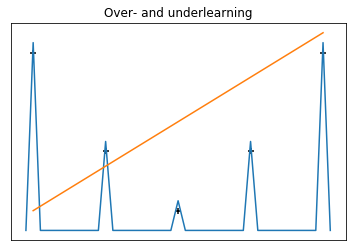
\includegraphics[width=0.6\linewidth]{over_and_underlearning}
	\caption{Illustration of over- and underlearning. The black crosses are the training samples. The straight line is the hypothesis learned by an underlearner, while the spiky line is the hypothesis learned by an overlearner.}
	\label{fig:over_and_underlearning}
\end{figure}

The key to a good $ERM_{\mathcal{H}}$ learner is a hypothesis class $\mathcal{H}$ with the right level of complexity,
\footnote{Other words for this nebulous concept include "capacity", "expressiveness", "richness", "expressive power", and "flexibility".}
not so big as to cause overlearning, but not so small as to cause underlearning. 

One useful definition of the complexity of a hypothesis class is its Vapnik--Chervonenkis dimension (VCdim), first proposed in 1968 \cite{vapnikUniformConvergenceRelative1971}. 

\begin{defn}\label{defn:shatter}
Given the feature space $\mathcal{X}$, binary label space $\mathcal{Y} = \{0, 1\}$, and a set of feature points $x_1, ... x_n \in \mathcal{X}$, a hypothesis class $\mathcal{H}$ \textbf{shatters} the set of feature points if, for any set of labels $y_1, ..., y_n\in \mathcal{Y}$, there exists a hypothesis $h\in\mathcal{H}$ such that 
$$h(x_i) = y_i, \quad \forall i \in [n]$$
\end{defn}

\begin{defn}\label{defn:VCdim}
For any hypothesis class $\mathcal{H}$ on the spaces $\mathcal{X}, \mathcal{Y}$, the \textbf{Vapnik--Chervonenkis dimension} of $\mathcal{H}$, written as $VCdim(\mathcal{H})$, is the size of the biggest subset of $\mathcal{X}$ that can be shattered by $\mathcal{H}$. If there is no maximal size, then $VCdim(\mathcal{H}) = \infty$.
\end{defn}

\subsection{The fundamental theorem of SLT}
Speculations about the meaning of life aside, the theory of PAC-learnability is very difficult, and the "fundamental theorem" concerns itself with only binary classification problems. That is, the label space  $\mathcal{Y} = \{0, 1\}$, and the loss function $\ell$ is the 0-1 loss.

Under such restrictive conditions, we have \cite[Theorem 6.7]{shalev-shwartzUnderstandingMachineLearning2014}:
\begin{theorem}
\label{theorem:funtheo_slt}
Given any learning problem $\mathcal{X}, \mathcal{Y} = \{0, 1\}$, with hypothesis class $\mathcal{H}$, and loss function being 0-1 loss, the following conditions are equivalent:
\begin{enumerate}[(1)]
	\item $\mathcal{H}$ is uniformly convergent. 
	\item $ERM_{\mathcal{H}}$ is a PAC-learner for this problem.
	\item This problem is PAC-learnable.
	\item $VCdim(\mathcal{H})$ is finite.
\end{enumerate}
\end{theorem}
\begin{proof}
	$(1) \Rightarrow (2)$: Proved in Proposition \ref{prop:uniconv}.
	
	$(2) \Rightarrow (3)$: Trivial.
	
	$(3) \Rightarrow (4)$: This step uses the \textit{no free lunch theorem}.
	
	$(4) \Rightarrow (1)$: There is a purely combinatorial proof, which we skip.
\end{proof}

Given any finite VC-dimensional hypothesis class, there are explicit bounds $n_{\mathcal{H}}(\epsilon, \delta)$ on how many samples the $ERM_\mathcal{H}$ learner need in order to accomplish PAC-learning, which are given quantitatively by combinatorial calculations in the $(4) \Rightarrow (1)$ step. We will not need explicit bounds in the proof. 

In order to complete the $(3) \Rightarrow (4)$ step, we present the no free lunch theorem. The proof can be found in \cite[Theorem 5.1]{shalev-shwartzUnderstandingMachineLearning2014}
\begin{theorem}[no free lunch]
\label{theorem:nfl}
Given any feature space $\mathcal{X}$, and binary sample space $\{0, 1\}$, let the loss function $\ell$ be 0-1 loss, then for any learner $Z^n \mapsto h_{Z^n}$ and any positive integer $n \le \frac 1 2 |\mathcal{X}|$ there exists a probability distribution $\mu$ on $\mathcal{X}\times\{0, 1\}$, so that there exists some 
$$h^* : \mathcal{X} \to \{0, 1\})$$
such that $\loss(h^*, \mu) = 0$, and yet
\begin{equation}
	\label{eq:nfl}
Pr_{Z^n \sim \mu^n}\left(\loss(h_{Z^n}, \mu) \ge \frac 1 8\right) \ge \frac 1 7
\end{equation}
\end{theorem}

Given the no free lunch theorem, we can complete the proof of Theorem \ref{theorem:funtheo_slt}:
\begin{proof}[Proof of $(3) \Rightarrow (4)$]
Suppose $(3)$ and not $(4)$. 

By $(3)$, PAC-learning is possible, so there exists some $n$, such that for any probability distribution $\mu$ on $\mathcal{X}\times\{0, 1\}$, we have PAC-learning

$$Pr_{Z^n \sim \mu^n}\left(\loss(h_{Z^n}, \mu) \ge \argmin_{h\in \mathcal{H}} \loss(h, \mu) + \frac 1 8\right) < \frac 1 7.$$

By not $(4)$, $VCdim(\mathcal{H}) = \infty$, and so there exists some $\{x_1, ..., x_n\}\in \mathcal{X}$ that is shattered by $\mathcal{H}$, that is, any partial hypothesis $h^* : \mathcal{X}\to \{0, 1\}$ can be realized by some $h$ in $\mathcal{H}$.

Then by no free lunch theorem, there exists a distribution $\mu$ on $\{x_1, ..., x_n\}\times\{0, 1\}$, such that, after extending $\mu$ to the rest of $\mathcal{X}\times \{0, 1\}$, satisfies 
$$\argmin_{h\in \mathcal{H}} \loss(h, \mu) = 0, $$ 
$$Pr_{Z^n \sim \mu^n}\left(\loss(h_{Z^n}, \mu) \ge  \frac 1 8\right) \ge \frac 1 7.$$

This is a contradiction.
\end{proof}

\subsection{Generalization to \cvar}\label{sec:slt_cvar}
The fundamental theorem of SLT can be easily generalized by replacing expectations with \cvar, after an appropriate generalization of PAC-learnability to arbitrary risk measures.

\begin{defn}[$\mathcal{F}$-expected loss function]
For any risk measure $\mathcal{F}: \mathscr{L} \to \mathbb{R}$ on real random variables, not necessarily the expectation or \cvar, we define a generalized expected loss function. For any hypothesis $h$ and distribution $\mu$ on $\mathcal{X}\times\mathcal{Y}$, 
\begin{equation}
\loss_\mathcal{F}(h, \mu) = \mathcal{F}(\ell(h(X), Y))
\end{equation}
where $\ell(h(X), Y)$ is a random variable with $(X, Y)\sim\mu$.
\end{defn}

By replacing $\loss$ with $\loss_\mathcal{F}$ in their definitions, we can generalize PAC-learnability, $\epsilon$-representativeness, uniform convergence, and empirical risk minimization for any $\mathcal{F}$, not just $\mathbb{E}$. 

The no free lunch theorem generalizes almost for free, despite its name:
\begin{theorem}[Generalized no free lunch]
\label{theorem:nfl_2}
Let $\mathcal{F}$ be any risk averse risk measure, that is, $\mathcal{F} \ge \mathbb{E}$. Given any feature space $\mathcal{X}$, and binary sample space $\{0, 1\}$, let the loss function $\ell$ be 0-1 loss, then for any learner $Z^n \mapsto h_{Z^n}$ and any positive integer $n \le \frac 1 2 |\mathcal{X}|$ there exists a probability distribution $\mu$ on $\mathcal{X}\times\{0, 1\}$, so that there exists some 
$$h^* : \mathcal{X} \to \{0, 1\})$$
such that $\loss_\mathcal{F}(h^*, \mu) = 0$, and yet
\begin{equation}
	\label{eq:nfl_2}
	Pr_{Z^n \sim \mu^n}\left(\loss_\mathcal{F}(h_{Z^n}, \mu) \ge \frac 1 8\right) \ge \frac 1 7
\end{equation}
\end{theorem}
\begin{proof}
Since $\loss \le \loss_\mathcal{F}$, the original no free lunch theorem immediately gives the result.
\end{proof}

Finally, we define a temporary notation, used only in the next theorem:
\begin{notn}
For any law invariant risk measure $\mathcal{F}: \mathscr{L} \to \mathbb{R}$, let $f_\mathcal{F} : [0, 1] \to \mathbb{R}$ be the function
$$f_\mathcal{F}(p) = \mathcal{F}(X)$$
where $X$ is a random variable with 
$$Pr(X = 0) = 1-p, \quad Pr(X = 1) = p$$
\end{notn}

Now, the fundamental theorem of SLT can be generalized to:

\begin{theorem}[Generalized fundamental theorem of SLT]
	\label{theorem:funtheo_slt_2}
Given any law invariant risk measure $\mathcal{F}$ with continuous $f_\mathcal{F}$, any learning problem $\mathcal{X}, \mathcal{Y} = \{0, 1\}$, with hypothesis class $\mathcal{H}$, and loss function being 0-1 loss, the following conditions are equivalent:
	\begin{enumerate}[(1)]
		\item $\mathcal{H}$ is $\mathcal{F}$-uniformly convergent. 
		\item $\mathcal{F}$-$ERM_{\mathcal{H}}$ is a $\mathcal{F}$-PAC-learner for this problem.
		\item This problem is $\mathcal{F}$-PAC-learnable.
		\item $VCdim(\mathcal{H})$ is finite.
	\end{enumerate}
\end{theorem}
\begin{proof}
$(1) \Rightarrow (2)$: This holds for all $\mathcal{F}$. The proof is the same as in Proposition \ref{prop:uniconv}.

$(2) \Rightarrow (3)$: This holds for all $\mathcal{F}$. The proof is immediate by definition of $\rho$-PAC-learnability.

$(3) \Rightarrow (4)$: This holds for all risk averse $\mathcal{F}$, that is, $\mathcal{F} \ge \mathbb{E}$, by the generalized no free lunch theorem.


$(4) \Rightarrow (1)$: By the original fundamental theorem of SLT, $\mathcal{H}$ is uniformly convergent, so it suffices to show it implies $\mathcal{H}$ is $\mathcal{F}$-uniformly convergent.

For any $\mu$, $\loss_\mathcal{F}(h, \mu) = \mathcal{F}(\ell(h(X), Y))$, where $(X, Y) \sim \mu$. Let the binary random variable $\ell(h(X), Y)$ have $Pr(\ell(h(X), Y) = 1) = p$, then $\loss(\ell(h(X), Y)) = p$, and so 
$$\loss_\mathcal{F}(\ell(h(X), Y)) = f_\mathcal{F}(p) = f_\mathcal{F}(\loss(\ell(h(X), Y)))$$

$f_\mathcal{F}$ is continuous on $[0, 1]$, so it is uniformly continuous, so for any $\epsilon>0$, there exists $\epsilon'$, such that any $\epsilon'$-representative training data $Z^n$ is $\epsilon$-$\mathcal{F}$-representative:

$$\forall h \in\mathcal{H}, \: |\loss(h, \mu_{Z^n}) - \loss(h, \mu)| \le \epsilon'$$ 
$$\Rightarrow \: |\loss_\mathcal{F}(h, \mu_{Z^n}) - \loss_\mathcal{F}(h, \mu)| = |f_\mathcal{F}(\loss(h, \mu{Z^n})) - f_\mathcal{F}(\loss(h, \mu))| \le \epsilon$$

Thus, if $\mathcal{H}$ is uniformly convergent, it has some $n_\mathcal{H}: (0, 1)\times (0, 1) \to \mathbb{N}$ such that $\forall \epsilon', \delta \in (0, 1), n \ge n_\mathcal{H}(\epsilon', \delta), $
$$Pr_{Z^n\sim \mu^n}(Z^n \text{ is }\epsilon'\text{-representative}) \ge 1-\delta$$
$$\Rightarrow Pr_{Z^n\sim \mu^n}(Z^n \text{ is }\epsilon\text{-}\mathcal{F}\text{-representative}) \ge 1-\delta$$
Thus $\mathcal{H}$ is $\mathcal{F}$-uniformly convergent.
\end{proof}

Moreover, given $\mathcal{F}$ and its function $f_\mathcal{F}$, an explicit bound on how many samples the ERM learner need in order to do PAC-learning can be given.

\begin{lemma}
For any spectral risk measure $\mathcal{F} = \int_0^1 \cvar_\alpha dm(\alpha)$ defined by a probability distribution $m$ on $[0, 1)$, its $f_\mathcal{F}$ is continuous.
\end{lemma}
\begin{proof}
By definition of $\cvar_\alpha$, we have $f_{\cvar_\alpha} = f_\alpha$, where 
$$f_\alpha(p) = \min{\left(\frac{p}{{{1}-\alpha}},{1}\right)}$$


In particular, since all $f_\alpha$ are concave and monotonically increasing on $[0, 1]$, their integral $f_\mathcal{F}$ is also. Since $f_\mathcal{F}$ is concave on $(0, 1)$, it is continuous there \cite[Theorem 1.5]{artinGammaFunction2015}.

For any $p\in(0, 1)$, and any $n > 1$, 
\begin{align*}
{{f}_{\mathcal{F}}{\left(\frac{p}{{n}}\right)}} &= \int_{{{\left[{0},{1}\right)}}}\min{\left(\frac{{\frac{p}{{n}}}}{{{1}-\alpha}},{1}\right)}{d}{m}{\left(\alpha\right)}\\
&= \int_{{{\left[{0},{1}-{p}\right)}}}\frac{{\frac{p}{{n}}}}{{{1}-\alpha}}{d}{m}{\left(\alpha\right)}+\int_{{{\left[{1}-{p},{1}-\frac{p}{{n}}\right)}}}{ \frac{{\frac{p}{{n}}}}{{{1}-\alpha}} }{d}{m}{\left(\alpha\right)}+\int_{{{\left[{1}-\frac{p}{{n}},{1}\right)}}}{1}{d}{m}{\left(\alpha\right)} \\
&\le \int_{{{\left[{0},{1}-{p}\right)}}}\frac{{\frac{p}{{n}}}}{{{1}-\alpha}}{d}{m}{\left(\alpha\right)}+\int_{{{\left[{1}-{p},{1}-\frac{p}{{n}}\right)}}}{1}{d}{m}{\left(\alpha\right)}+\int_{{{\left[{1}-\frac{p}{{n}},{1}\right)}}}{1}{d}{m}{\left(\alpha\right)} \\
&= \displaystyle\frac{p}{{n}}\int_{{{\left[{0},{1}-{p}\right)}}}\frac{1}{{{1}-\alpha}}{d}{m}{\left(\alpha\right)}+{m}{\left({\left[{1}-{p},{1}\right)}\right)}
\end{align*}

Thus, $0 \le \limsup_{p\to 0} f_\mathcal{F}(p)\le \inf_{p\in(0, 1)} m([1-p, 1)) = 0$. So $f_\mathcal{F}$ is continuous at $0$.

Finally, at $p\to 1$, since $f(p)$ is monotonically increasing, any discontinuity there can only be a jump upwards. Since $f_\mathcal{F}$ is also concave on $[0, 1]$, it cannot have it, so $f_\mathcal{F}$ is continuous at $1$.
\end{proof}

\begin{cor}
For any spectral risk measure $\mathcal{F} = \int_0^1 \cvar_\alpha dm(\alpha)$ defined by a probability distribution $m$ on $[0, 1)$, it satisfies the generalized fundamental theorem of SLT.
\end{cor}

We give an explicit quantitative illustration:
\begin{ex}
For any $\alpha\in(0, 1)$, $f_{\cvar_\alpha}$ has the modulus of continuity $\frac{1}{1-\alpha}$, so any $\epsilon$-representative sample $Z^n$ is a $\frac{\epsilon}{1-\alpha}$-$\mathcal{F}$-representative sample. 

By combining \cite[Theorem 6.10, 6.11]{shalev-shwartzUnderstandingMachineLearning2014}, if $\mathcal{H}$ has finite VC-dimension $d$, then for all $n\in\mathbb{N}$, 
$$Pr_{Z^n \sim \mu^n}\left(Z^n \text{ is } 
g(n)
\text{-representative}\right) \ge 1-\delta$$
where
$$g(n) = \frac{{{4}+\sqrt{{{d}{\left( \ln{{\left({2}{n}\right)}}- \ln{{d}}+{1}\right)}}}}}{{\delta\sqrt{{{2}{n}}}}}$$ 
Thus, 
$$Pr_{Z^n \sim \mu^n}\left(Z^n \text{ is } 
\displaystyle\frac{ g{{\left({n}\right)}}}{{{1}-\alpha}} \text{-}\mathcal{F}\text{-representative}\right) \ge 1-\delta$$

Since $\lim_n g(n) = 0$, for any $\epsilon, \delta \in (0, 1)$, take any $N$ such that $2 g(N) < \frac{\epsilon}{{{1}-\alpha}}$, then for any $n > N$, 
$$Pr_{Z^n \sim \mu^n}\left(Z^n \text{ is } 
\frac \epsilon 2 \text{-}\mathcal{F}\text{-representative}\right) \ge 1-\delta$$
So, taking $n$ training samples allows ERM to do $\mathcal{F}$-PAC-learning:
$$Pr_{Z^n \sim \mu^n}\left(\loss_\mathcal{F}(h_{Z^n}, \mu) \le \min_{h\in\mathcal{H}}\loss_\mathcal{F}(h, \mu) + \epsilon\right) \ge 1-\delta.$$
\end{ex}

  
\chapter{Limit theorems of coherent risk measures}
\label{chapter_clt}

In this chapter, we start by reviewing limit theorems in probability and large deviation theory, then move on to a new proof of the central limit theorem (CLT) for an empirical process of \cvar, which generalizes the classical CLT for expectation.

In the literature, there have been generalizations of limit theorems results to \cvar. In particular, \cite{chenNonparametricEstimationExpected2007} proves the generalized central limit theorem, and \cite{gaoAsymptoticBehaviorEmpirical2011}, the generalized Berry--Esseen inequality, law of iterated logarithm, and large and moderate deviation principles.  However, the proof presented below of the CLT of \cvar is new, as far as we are aware.

\section{Limit theorems in probability}
In calculus, each convergent real sequence $(x_n)$ has a limit $x_\infty$ associated with it. Taking the limit is a lossy operation that loses most of the details, but preserves something essential about the sequence $(x_n)$, namely, its \textit{eventual} behavior.

In probability, given a stochastic process $(Y_n)$, one may ask if there exists some random variable or real number (which is a degenerate random variable) as its limit. The answer is yes, in certain senses. Making this precise gives us the limit theorems.


The most important limit theorems are the central limit theorem (CLT), the weak law of large number (WLLN), and the strong law of large number (SLLN).

\subsection{Central limit theorem (CLT)}
There are many formulations of CLT, but we will only need the classical CLT \cite[Theorem 27.1]{billingsleyProbabilityMeasure2012}:
\begin{theorem}[classical CLT]
Suppose that $(X_n)$ is an independent sequence of random variables having the
same distribution with finite mean $\mu$ and variance $\sigma^2$. If $\overbar{X_n} = \frac 1 n (X_1 + \cdots +X_n)$, then 
\begin{equation}
\label{eq:clt}
\sqrt{n}\, (\overbar{X_n} - \mu)
\distconv \mathcal{N}(0, \sigma^2)
\end{equation}
\end{theorem}

Here, $\mathcal{N}$ denotes the normal distribution:
\begin{defn}\label{defn:normal_dist}
	For any $\mu\in \mathbb{R}, \nu > 0$, $\mathcal{N}(\mu, \nu)$ is the standard normal distribution with mean $\mu$ and variance $\nu$, with PDF
	\begin{equation}
	\rho(x) = \frac{1}{\sqrt{2\pi}} e^{-x^2/2}.
	\end{equation}
\end{defn}

As noted in Example \ref{ex:IID_average}, the CLT can be rephrased in the language of empirical process $(L_n)$ of $X$:

\begin{equation}
\label{eq:clt_2}
\sqrt{n}\, (\mathbb{E}(L_n) - \mathbb{E}(X)) \distconv \mathcal{N}(0, 1)
\end{equation}

This immediately suggests the generalization 
\begin{equation}\label{eq:cvar_clt}
\sqrt{n}\, (\cvar_\alpha(L_n) - \cvar_\alpha(X)) \distconv \mathcal{N}(0, \sigma(\alpha))
\end{equation}
where $0 \le \alpha < 1$, and $\sigma(\alpha)$ is a function that possibly depends on $\alpha$ and $X$. 

At $\alpha = 0$, this reduces to the original CLT, and so $\sigma(0)= 1$. At $\alpha = 1$, 
$$\cvar_\alpha(L_n) - \cvar_\alpha(X) = \max_{i\in[n]}X_i \esssup(X)> 0$$ 
has probability zero, and so the generalized CLT cannot be true.

As will be shown in Theorem \ref{theorem:clt_cvar}, except at points of $\alpha$ where $F_X^{-1}(\alpha)$ is discontinuous, this generalization (Equation \ref{eq:cvar_clt}) is indeed true.

\subsection{Strong laws of large numbers (SLLN)}

\begin{theorem}[Laws of large numbers for expectations]
If $\mathbb{E}(|X|)< \infty$, that is, $X\in \mathscr{L}^1$, then  $\mathbb{E}(L_n)$ converges to $\mathbb{E}(X)$, in the senses of:
\begin{enumerate}[(1)]
	\item (Weak law) convergence in probability.
	\item (Strong law) almost sure convergence.
\end{enumerate}
\end{theorem}

Both CLT and SLLN are "stronger" than WLLN, in that any random variable $X$ that satisfies CLT or SLLN would satisfy WLLN. However, CLT and SLLN do not imply each other in general. As it is a corollary of SLLN, we will not mention WLLN any longer.

\begin{theorem}[SLLN for \cvar]
For any real random variable $X$, and any $0\le \alpha \le 1$, $\cvar_\alpha(L_n)$ converges to $\cvar_\alpha(X)$ almost surely.
\end{theorem}

For the case of $\alpha = 0$, this is the usual case of the SLLN. For the case of $\alpha=1, \cvar_1 = \esssup$, and the proof is easy. The general case is Theorem \ref{thm:slln_cvar}, deferred to Section \ref{sec:slln_for_cvar}.
\begin{theorem}[SLLN for $\esssup$]
	\label{theorem:slln_esssup}
For any real random variable $X$,  $\esssup(L_n)$ converges to $\esssup(X)$ almost surely.
\end{theorem}
\begin{proof}
First, the case of $\esssup(X)<\infty$: For any $n\in\mathbb{N}$, 
$\esssup(L_n) = \max(X_1, ..., X_n)$, so $(\esssup(L_n))_n$ is a non-decreasing sequence. 

By definition of essential supremum, $Pr(\esssup(L_n) \le \esssup(X)) = 1$, so the sequence almost surely converges to a limit less or equal to $\esssup(X)$, and it suffices to show $Pr(\limsup_n (\esssup(L_n) - \esssup(X)) \ge 0) = 1$.

For any $\epsilon > 0$, 
$$Pr(\esssup(L_n) < \esssup(X)-\epsilon) = Pr(X<\esssup(X)-\epsilon)^n\to 0$$

Thus,  $Pr(\lim_n (\esssup(L_n) - \esssup(X)) \ge -\epsilon) = 1$ for all $\epsilon > 0$, and so $Pr(\limsup_n (\esssup(L_n) - \esssup(X)) \ge 0) = 1$.

For the case of $\esssup(X)=\infty$, the same proof applies, after replacing $\esssup(X)-\epsilon$ by $M$, an arbitrarily big number.
\end{proof}


\subsection{Law of the iterated logarithm (LIL)}
Lying between SLLN and CLT is the law of the iterated logarithms (LIL). With no loss of generality, consider a random variable $X$ with mean $0$ and variance $1$, and $(X_n)_n$ being its IID process. SLLN states that $\frac 1 n \sum_{i = 1}^n X_i \asconv 0$, that is, the distribution of $\frac 1 n \sum_{i = 1}^n X_i$ converges to $\delta_0$ "quickly". CLT states that the distribution of $\frac{1}{\sqrt{n}} \sum_{i = 1}^n X_i$ converges to $\mathcal{N}(0, 1)$. 

Intermediate between them, LIL states that $\frac{1}{\sqrt{n\ln\ln{n}}} \sum_{i = 1}^n X_i$ converges to $\delta_0$, but slowly, so that $\limsup_n \frac{1}{\sqrt{n\ln\ln{n}}} \sum_{i = 1}^n X_i = \sqrt{2}$ almost surely.

\begin{theorem}[Law of the iterated logarithms]
Given random variable $X$ with mean $0$ and variance $1$, and $(X_n)_n$ being its IID process, then
\begin{equation}
\limsup_n \frac{1}{\sqrt{n\ln\ln{n}}} \sum_{i = 1}^n X_i = \sqrt{2} \text{ almost surely.}
\end{equation}
By symmetry, we also have 
\begin{equation}
\liminf_n \frac{1}{\sqrt{n\ln\ln{n}}} \sum_{i = 1}^n X_i = -\sqrt{2} \text{ almost surely.}
\end{equation}
\end{theorem}

Pictorially, one can consider a random walk process $(S_n)_n$ defined by $S_n =  \sum_{i = 1}^n X_i$, shown in Figure \ref{fig:lil}.


\begin{figure}
	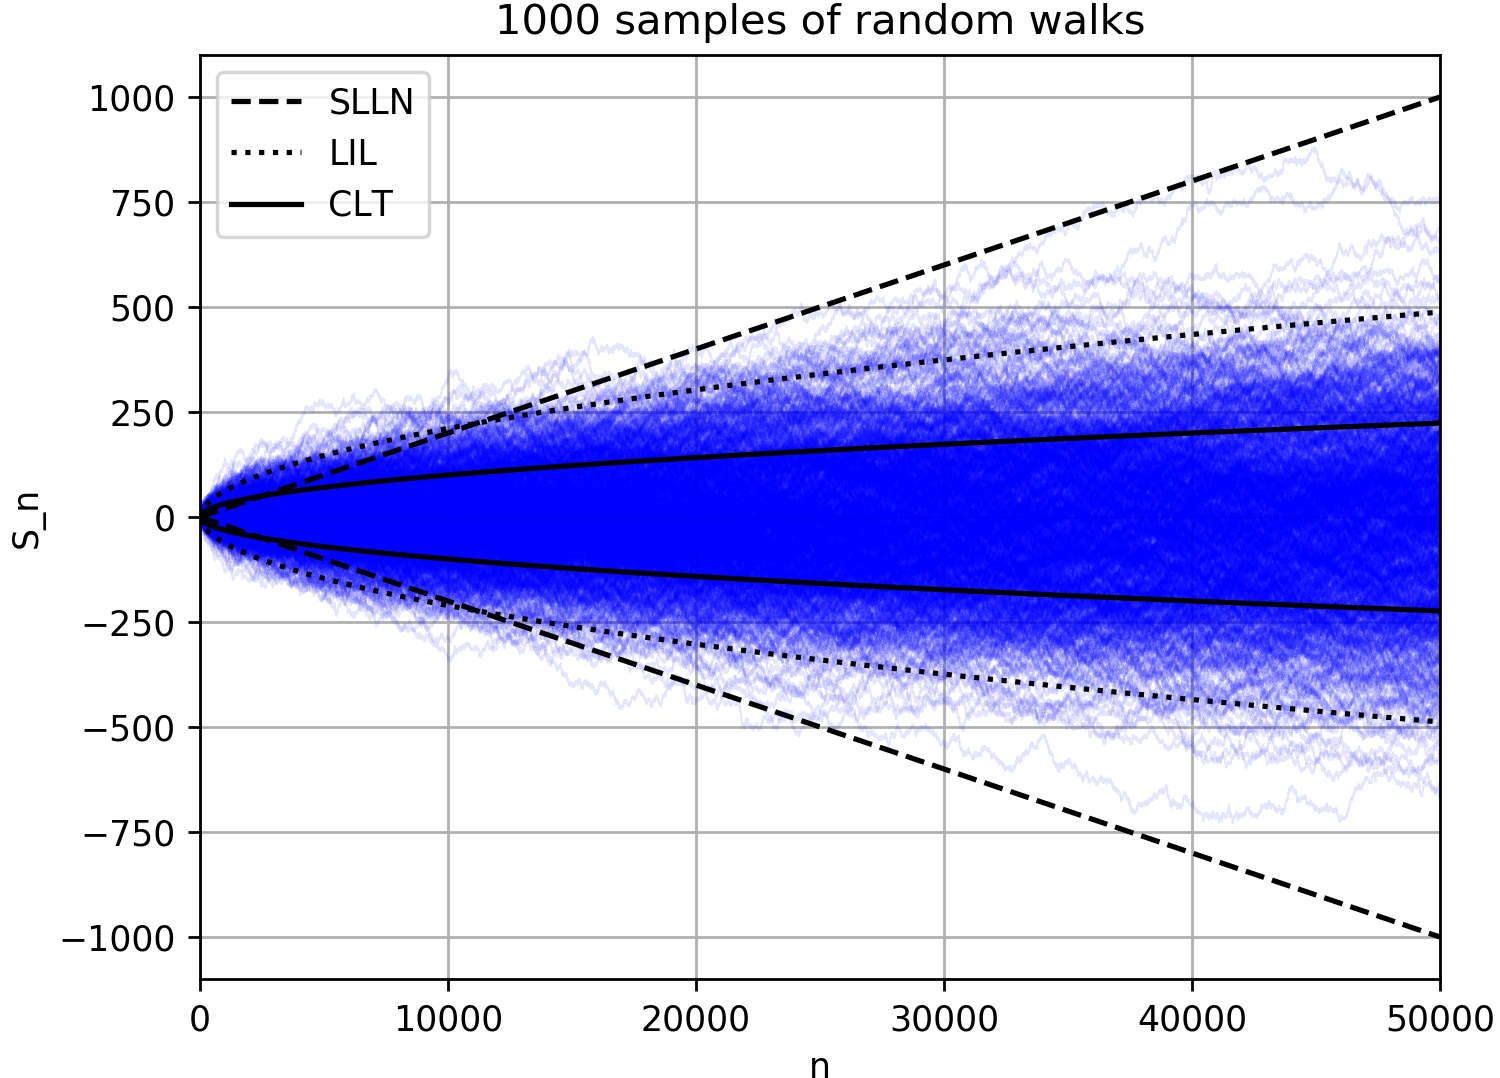
\includegraphics[width=\linewidth]{1000_random_walks}
	\caption{$1000$ samples of random walks, with each step having mean $0$ and variance $1$. Almost all the walks eventually fall inside the outer dashed cone of $y = \pm \epsilon n$, demonstrating the SLLN. Most of the walks barely touch the edges of the cone $y = \pm \sqrt{2 n \ln\ln{n}}$, demonstrating the LIL. About 68\% of the walks are inside the cone $y = \pm \sqrt{n }$ at the right edge of the graph, demonstrating one instance of the CLT.}
	\label{fig:lil}
\end{figure}

SLLN states that for any $\epsilon > 0$, with probability one, a randomly chosen walk would eventually be contained in the cone $y = \pm \epsilon x$.

CLT states that for any $\epsilon > 0$, for big $n$, the probability that a randomly chosen path is within the cone $y = \pm \epsilon \sqrt{x}$ at the $x = n$ section (that is, $S_n \in (-\epsilon \sqrt{x}, \epsilon \sqrt{x})$) is $Pr(\mathcal{N}(0, 1)\in (-\epsilon, \epsilon))$.

Intermediately, LIL states that with probability one, a random path would touch the edge of the cone $y = \pm \sqrt{2 x \ln\ln{x}}$ infinitely many times, but for any $\epsilon > 0$, it would only touch the edge of $y = \pm (1+\epsilon )\sqrt{2 x \ln\ln{x}}$ finitely many times.

While SLLN and CLT are extensively used in practical statistics, the LIL in comparison has little practical consequence \cite{vandervaartAsymptoticStatistics2000}. One classic paper on applications of LIL to statistics is \cite{robbinsStatisticalMethodsRelated1970}.

Before plunging into large deviation theory, which we will use to derive the CLT for certain risk measures, we take note of the surrounding territory for context.

In the literature, one can often find mentions of \textbf{large/moderate/small deviation principles}. Among these, the \textit{large} deviation principles are the most popular. Two standard references on this subject are \cite{demboLargeDeviationsTechniques2009, denhollanderLargeDeviations2008}.

\subsection{Deviation principles}
Consider a random variable $X$ with mean $0$ and variance $1$, and its IID process $(X_n)_n$. Let $S_n = X_1 + \cdots + X_n$. By the CLT, we have for any constant $\epsilon > 0$, 
\begin{equation}
\lim_n Pr(S_n > \epsilon n^{\frac 1 2}) = 1 - \Phi(\epsilon),
\end{equation}
where $\Phi$ is the CDF of the standard normal distribution.

If $|X|$ has finite third moment, then by the Berry--Esseen theorem \cite[Theorem 3.4.9]{durrettProbabilityTheoryExamples2010}, this convergence is uniform in the sense that 
\begin{equation}
\lim_n \frac {Pr(S_n > x_n n^{\frac 1 2})}  {1 - \Phi(x_n)} = 1
\end{equation}
for any sequence of $(x_n)_n$ that satisfies $x_n = O(1)$. This, though not often called so, is a \textit{small} deviation principle.

One immediately considers generalization for $x_n$ that may grow faster than $O(1)$. 

The large deviation theorem would give an asymptotic expansion in the case where $x_n$ is $O(n^{\frac 1 2})$. For example, Cram\'er's theorem states that if $X$ is "nice", there exists a \textbf{rate function} $I : \mathbb{R} \to [0, \infty)$ such that 

$$\forall \epsilon > 0, \: 
Pr(S_n > \epsilon n) \to e^{-nI(\epsilon)}.$$

More rigorously, the convergence is 
\begin{equation}
\frac 1 n \ln Pr(S_n > \epsilon n) \to -I(\epsilon).
\end{equation}

Between them, a moderate deviation theorem \cite{chenSteinIdentitiesModerate2013} states that the asymptotic expansion is
\begin{equation}
	\frac {Pr(S_n > x_n n^{\frac 1 2})}  {1 - \Phi(x_n)} = 1 + O(1) \frac{1 + x^3_n}{\sqrt{n}}.
\end{equation}
for $x_n = O(n^{\frac 1 6})$. In more details, it states that 
\begin{equation}
	\left(\frac {Pr(S_n > x_n n^{\frac 1 2})}  {1 - \Phi(x_n)} - 1\right) \frac{\sqrt{n}}{1 + x^3_n}.
\end{equation}
is bounded as $n\to\infty$.

In \cite{rubinProbabilitiesModerateDeviations1965}, a moderate deviation defined by $x_n = O(\sqrt{\ln{n}})$ is studied. In general, moderate deviation studies 
$$O(1) < x_n < O(\sqrt{n}),$$
that is, 
\begin{equation}
|x_n| \to \infty, \: \frac{x_n}{\sqrt{n}} \to 0.
\end{equation}

A large part of modern probability consists of various generalizations of the deviation principles under assumptions on $(X_n)_n$ weaker than full independence
\footnote{Such as "weakly dependent", "strongly mixing", "exchangeable", "ergodic", and many other highly technical weakenings.}. The sequences of $(X_n)_n$ could also be generalized to be multidimensional, or graphs, or some other complicated mathematical objects.

\subsection{The G\"artner--Ellis theorem}
The G\"artner--Ellis theorem states a large deviation principle for sequences of not necessarily independent random variables. It uses a generalization of the cumulant generating function:

\begin{defn}
For any real random variable $X$, its \textbf{cumulant generating function} is
\begin{equation}
\forall t\in \mathbb{R}, \quad K(t) = \ln\mathbb{E}(e^{tX}).
\end{equation}
\end{defn}


Consider, for example, the empirical process $(L_n)$ of $X$, and the sequence $\mathbb{E}(L_n) = \frac 1 n \sum_{i=1}^n X_i$, then we have 
$${\mathbb{{{E}}}}{\left({e}^{{{n}{t}{\mathbb{{{E}}}}{\left({L}_{{n}}\right)}}}\right)} = {\mathbb{{{E}}}}{\left({e}^{{{t}{X}}}\right)}^{n}
$$
and so for any $t\in\mathbb{R}$,
$$K(t) = \lim_{n\to \infty}\frac 1 n \ln {\mathbb{{{E}}}}{\left({e}^{{{n}{t}{\mathbb{{{E}}}}{\left({L}_{{n}}\right)}}}\right)}$$

For a general sequence of real random variables, $(Y_n)_n$, let 
$$K_n(t) = \frac 1 n \ln {\mathbb{{{E}}}}{\left({e}^{{{n}{t}{\mathbb{{{E}}}}{\left({L}_{{n}}\right)}}}\right)},$$
then if the following limit exists
$$\lim_{n\to \infty}K_n(t)$$
for all $t$ in a neighborhood of $0$, then the G\"artner--Ellis theorem gives the limit behavior of a properly scaled version of the sequence $(Y_n)_n$.

There are many versions of the G\"artner--Ellis theorem with varying generalities. The version that we use is \cite[Lemma 1]{coxLargeDeviationsPoisson1984}:
\begin{theorem}[G\"artner--Ellis theorem]
\label{theorem:gartner}
For a general sequence of real random variables, $(Y_n)_n$, if the following limit exists
$$K(t) = \lim_{n\to \infty}\frac 1 n \ln \displaystyle{\mathbb{{{E}}}}{\left({e}^{{{n}{t}{Y}_{{n}}}}\right)}$$
for $t$ in a neighborhood $(\epsilon_-, \epsilon_+)$ of $0$, and if $K$ is strictly convex and $C^2$ on $(\epsilon_-, \epsilon_+)$, then, letting $\mu = K'(0), \sigma^2 = K''(0)$,
\begin{enumerate}[(1)]
	\item (SLLN) $Y_n \asconv \mu$.
	\item (CLT) If for all sufficiently large $n$, $K_n$ is convex on $[0, \epsilon_+)$, and $\lim_n K_n''(0) = \sigma^2$, then \begin{equation}
		\frac{Y_n - \mathbb{E}(Y_n)}{\sqrt{n}} \distconv \mathcal{N}(0, \sigma^2).
	\end{equation}
%	\item (LDP) Let $\mu_+ = K'(\epsilon_+), \mu_- = K'(\epsilon_-)$, then for all $\zeta\in(\mu, \mu_+)$, \begin{equation}
%		\lim_n \frac 1 n \ln Pr\left(\frac{Y_n}{n} > \zeta\right) = -K^*(\zeta)
%	\end{equation}
%	and similarly for all $\zeta\in(\mu_-, \mu)$, \begin{equation}
%	\lim_n \frac 1 n \ln Pr\left(\frac{Y_n}{n} < \zeta\right) = -K^*(\zeta)
%	\end{equation}
\end{enumerate}
\end{theorem}

\section{Limit theorems of \cvar}
In this section, we present calculations and numerical evidence that demonstrate, if not prove with full rigor, the CLT and SLLN of \cvar.

\subsection{CLT for \cvar}
\label{sec:clt_cvar}

Consider a real $X$ with PDF $\rho$ and CDF $\Phi$. For any $h \in \mathbb{N}$, define 
\begin{align*}
\label{eq:temp_1}
\mathbb{E}(\exp{(nt \cvar_\alpha(L_n))}) &= \mathbb{E}\left(\exp{\left( \frac{t}{\overbar{\alpha}} \sum_{i=1}^{\overbar{\alpha} n} X_{(i)} \right)}\right) \\
&= \mathbb{E}\left(\exp{\left( \frac{t}{\overbar{\alpha}} \sum_{i=1}^{\overbar{\alpha} n} X_i \right)} \Big| X_1, ..., X_{\overbar{\alpha} n} > X_{\overbar{\alpha} n + 1} > X_{\overbar{\alpha} n + 2} , ... X_n\right) 
\end{align*}
Here, $X_{(i)}$ denotes the i-th biggest term in the sequence $X_1, ... X_n$. The cases where two or more $X_i$ are equal having measure $0$, thus ignored.

Note that the sum should not be taken literally, as in actuality, $\cvar_\alpha(L_n)$ is the average of the biggest $\floor{\overbar{\alpha} n}$ terms of $X_1, ..., X_n$, plus $\{\overbar{\alpha} n\}$ times the next biggest term. However, as $n$ grows, this little fudge factor will be swamped out, and therefore we ignore it.

That the expectation can be conditioned on a particular choice of ordering of $X_i$ is because the sequence $(X_n)_n$ is an \textbf{exchangeable sequence of random variables}, that is, any finite permutation of the sequence creates a sequence with the same distribution.

Now we continue the calculation.
\begin{align*}
&= \int_{\mathbb{R}} Pr(X_{\overbar{\alpha} n + 1}\in dx |  X_1, ..., X_{\overbar{\alpha} n} > X_{\overbar{\alpha} n + 1} > X_{\overbar{\alpha} n + 2} , ... X_n) \mathbb{E}(e^{\frac{tX}{\overbar{\alpha}}} | X > x)^{\overbar{\alpha} n} \\
&= \int_{\mathbb{R}} 
\frac{F_X(x)^{\alpha n - 1}(1-F_X(x))^{\overbar{\alpha} n} \rho(x) dx}{B(\alpha n, \overbar{\alpha} n + 1)}
\mathbb{E}(e^{\frac{tX}{\overbar{\alpha}}} | X > x)^{\overbar{\alpha} n}
\end{align*}
where $B(x, y) = \frac{\Gamma(x)\Gamma(y)}{\Gamma(x+y)}$ is the Euler beta function, and $\Gamma$ is the Euler gamma function.

Plugging in 
$$(1-F_X(x))\mathbb{E}(e^{\frac{tX}{\overbar{\alpha}}} | X > x) = \int_x^\infty  e^{ty/\overbar{\alpha}} \rho(y)dy, $$
we obtain
\begin{align*}
&= \frac{1}{B(\alpha n, \overbar{\alpha} n + 1)}\int_{\mathbb{R}} 
\left(F_X(x)^\alpha \left(\int_x^\infty  e^{ty/\overbar{\alpha}} \rho(y)dy\right)^{\overbar{\alpha}}\right)^n
\frac{\rho(x)}{F_X(x)}dx
\end{align*}

Now, by Stirling's approximation, 
$$B(\alpha n, \overbar{\alpha} n + 1) = \exp(-n H(\alpha) + O(\ln n)),$$
where 
\begin{equation}
H(\alpha) = -\alpha \ln \alpha - \overbar{\alpha} \ln \overbar{\alpha}
\end{equation} 
is the binary entropy function.

So, by Laplace's method 
\cite[Section 6.4]{benderAdvancedMathematicalMethods1999}, 
\begin{equation}
K(t) = H(\alpha) + \max_{x\in\mathbb{R}}
\left(\alpha \ln F_X(x)
+
\overbar{\alpha}\ln\left(\int_x^\infty  e^{ty/\overbar{\alpha}} \rho(y)dy\right)\right)
\end{equation}
provided that 
\begin{equation}
	\label{eq:maxfun}
\alpha \ln F_X(x)
+
\overbar{\alpha}\ln\left(\int_x^\infty  e^{ty/\overbar{\alpha}} \rho(y)dy\right)
\end{equation}

has a unique global maximum at some $x_0$, is $C^2$ in a neighborhood of $x_0$, and $\frac{\rho(x_0)}{F_X(x_0)}> 0$. 

Taking derivative, such a maximum is a root of 
\begin{equation}
\label{eq:maxfun_root}
F_X(x) = \frac{\alpha}{\overbar{\alpha}}\int_0^\infty e^{ty/\overbar{\alpha}}\rho(x+y)dy.
\end{equation}
At $ t = 0$ has solution $x = F_X^{-1}(\alpha)$, and we obtain
$$K(0) = H(\alpha) + \alpha \ln F_X(F_X^{-1}(\alpha)) + \overbar\alpha\ln\int_{F_X^{-1}(\alpha)}^\infty \rho(y)dy = 0$$
as it should.

Near $t=0$, $x$ can be expanded as a power series $x = F_X^{-1}(\alpha) + x_1 t + x_2 t^2 + o(t^2) $, which can then be plugged into the equation of $K(t) = \mu(\alpha) t + \frac 12 \sigma(\alpha)^2 + o(t^2)$, from which we obtain 
\begin{equation}
\sqrt{n}(\cvar_\alpha(L_n) - \mu(\alpha))\distconv \mathcal{N}(0, \sigma(\alpha)^2)
\end{equation}

\begin{ex}
$X$ is uniform on $[0, 1]$, then
\begin{equation}
K(t) = H(\alpha) + \max_{x\in(0, 1)}
\left(\alpha \ln x
+
\overbar{\alpha}\ln\frac{\overbar{\alpha}}{t}\left(e^{t/\overbar{\alpha}} - e^{tx/\overbar{\alpha}}\right)\right)
\end{equation}

The maximizer $x$ is the root of 
$$x = \frac{\alpha}{t}\left(e^{t(1-x)/{\overbar\alpha}} - 1\right)$$
which has asymptotic expansion 
$$x = \alpha + x_1 t + x_2 t^2 + o(t^2).$$
Plugging it in and solving up to $t^2$ order, we obtain 
$$ x = \alpha + \frac 12 \alpha{\overbar\alpha} t + \frac 16 \alpha{\overbar\alpha}(1-3\alpha) t^2 $$
and so 
$$K(t) = \frac 12 (1+\alpha) t + \frac{1}{24}(1-\alpha)(1+3\alpha)t^2 + o(t^2)$$
So we obtain the CLT for $X$:
\begin{equation}
\label{eq:uniform_std}
\mu(\alpha) = \frac 12 (\alpha+1) = \cvar_\alpha(X), \quad \sigma(\alpha)^2 = \frac{1}{12}(1-\alpha)(1+3\alpha)
\end{equation}

This is illustrated in Figures \ref{fig:cvar_uniform_clt} and \ref{fig:cvar_stds}.
\end{ex}

\begin{figure}
	\centering
	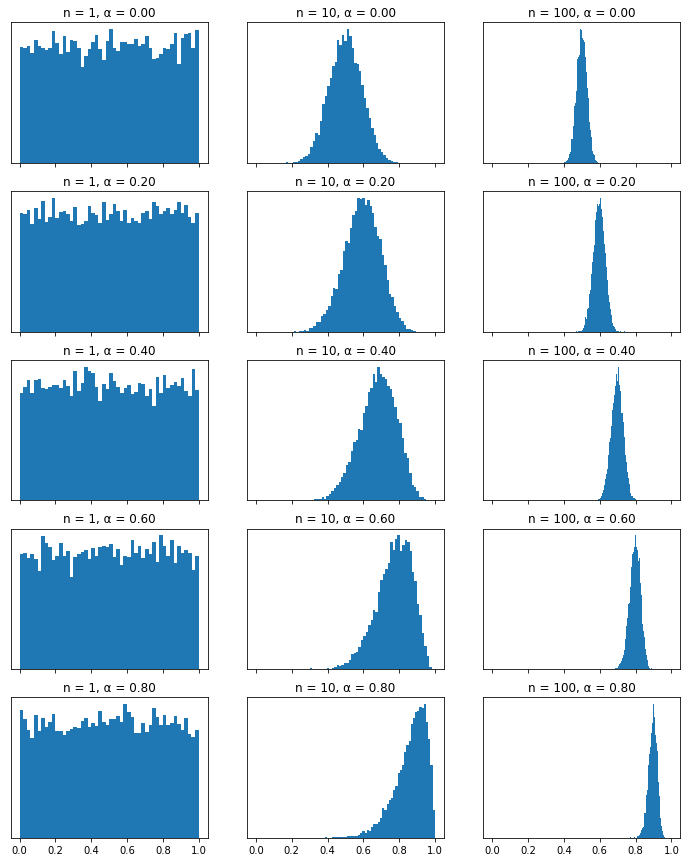
\includegraphics[width=0.9\textwidth]{cvar_uniform_clt.png}
	\caption{A demonstration of the CLT for \cvar. Here, $X$ is the uniform distribution on $[0, 1]$, and the PDF of $\cvar_\alpha (L_n)$ is plotted as a function of $n$ and $\alpha$. As $n$ increases, the distributions converge to normal distributions. Increasing $\alpha$ both shifts the distribution to the right, and distort it away from normality. Each histogram is the result of $10^4$ trials.}
	\label{fig:cvar_uniform_clt}
\end{figure}

\begin{figure}
	\centering
	\begin{subfigure}[b]{0.45\textwidth}
		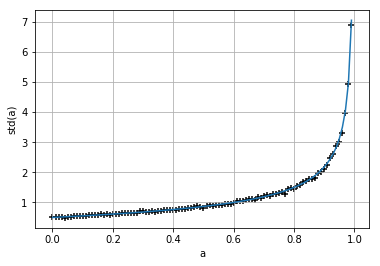
\includegraphics[width=\textwidth]{exponential_std.png}
		\caption{$\rho(x) = 2e^{-2x}$ with $x > 0$.}
		\label{fig:exp_std}
	\end{subfigure}
	~
	\begin{subfigure}[b]{0.45\textwidth}
		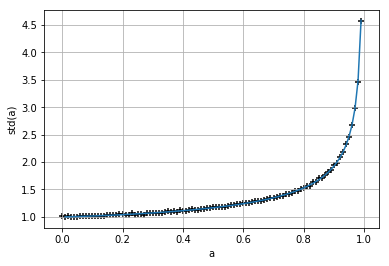
\includegraphics[width=\textwidth]{gaussian_std.png}
		\caption{$X\sim \mathcal{N}(0, 1)$.}
		\label{fig:gaussian_std}
	\end{subfigure}
	~
	\begin{subfigure}[b]{0.45\textwidth}
		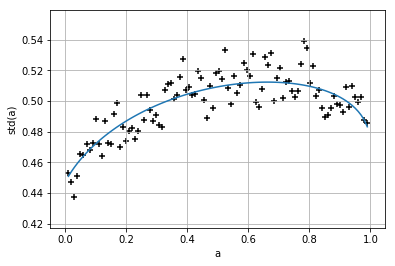
\includegraphics[width=\textwidth]{parabolic_std.png}
		\caption{$\rho(x) = \frac 34 (1-x^2)$ with $x\in[-1, 1]$}
		\label{fig:parabolic_std}
	\end{subfigure}
	~
	\begin{subfigure}[b]{0.45\textwidth}
		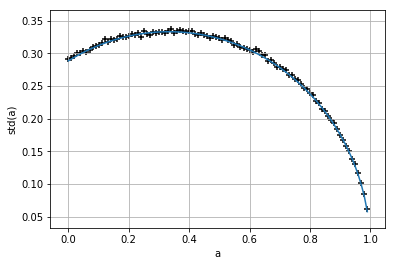
\includegraphics[width=\textwidth]{uniform_std.png}
		\caption{$X$ is uniform on $[0, 1]$.}
		\label{fig:uniform_std}
	\end{subfigure}
	~
	\begin{subfigure}[b]{0.45\textwidth}
		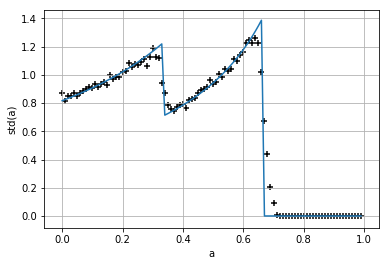
\includegraphics[width=\textwidth]{discrete_0_1_2_std.png}
		\caption{$X$ is discrete uniform on $\{0, 1, 2\}$.}
		\label{fig:discrete_0_1_2_std}
	\end{subfigure}
	~
	\begin{subfigure}[b]{0.47\textwidth}
		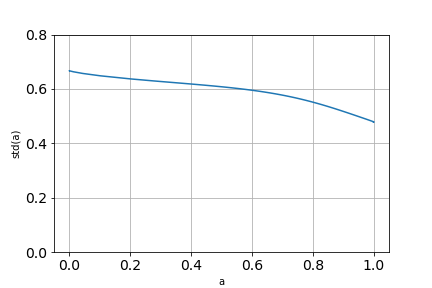
\includegraphics[width=\textwidth]{xex2_std.png}
		\caption{$\rho(x) = -xe^{-x^2/2}$ with $x< 0$.}
		\label{fig:xex2_std}
	\end{subfigure}
	\caption{Numerical confirmation of Theorem \ref{theorem:clt_cvar} (CLT for \cvar). $\sigma(\alpha)$ plots for six different distributions of $X$ are calculated, and five of them fits the numerical simulation. The last plot is calculated only theoretically, without numerical verification. The curves are the exact theoretical prediction of the standard deviation of $\sqrt{n}\cvar_\alpha(L_{n})$ as $n\to \infty$, given by Equation \ref{eq:clt_cvar}. Each point in the scatterplots is obtained by sampling $\sqrt{n}\cvar_\alpha(L_{n})$ for $1000$ times, where $n = 1000$. }
	\label{fig:cvar_stds}
\end{figure}

\begin{ex}
A discrete $X$ with a finite discrete distribution $\sum_{i = 1}^N p_i \delta_{x_i}$ can be approximated by very concentrated uniform distributions, that is, 
$$\rho(x) = \begin{cases}
\frac{p_i}{\epsilon}\quad x\in[x_i, x_i+\epsilon]\\
0 \quad \text{else}
\end{cases}, 
$$
where $\epsilon$ is a positive number smaller than $\min_{1 \le i \le N-1}(x_{i+1} - x_i)$.

Let $P_i = p_1 + ... + p_i$ for all $i\in [N]$, then if $\alpha \in (P_{i-1}, P_i)$ for some $i\in [N]$, then $F_X^{-1}(\alpha) =x_i + \frac{\epsilon}{p_i} (\alpha - P_{i-1})$. Then, the maximum in Equation \ref{eq:maxfun} is the root of 
$$P_{i-1} + \frac{p_i}{\epsilon}(x-x_i) = \frac{\alpha}{\epsilon t}
\left(p_i \left(e^{(\epsilon - (x-x_i))t/{\overbar\alpha}} - 1\right) + 
\sum_{j = i+1}^N \left(p_j e^{(x_j - x)t/{\overbar\alpha}} \left(e^{\epsilon t/{\overbar\alpha}} - 1\right) \right)\right)$$
which has the power expansion
$$ x =  x_i + \frac{\epsilon}{p_i} (\alpha - P_{i-1}) + A t + Bt^2 + o(t^2)$$

Plugging it in to solve for $A, B$, then expanding $K$, and taking the $\epsilon \to 0$ limit, we obtain 
$$K(t) = \mu(\alpha) t + \frac 12 \sigma(\alpha)^2 t^2$$ 
where
\begin{equation}
\mu(\alpha) = \frac{1}{{\overbar\alpha}}( x_i (P_i - \alpha) + \sum_{k > i}^N p_k x_k) = \cvar_\alpha(X), 
\end{equation}
\begin{equation}
\sigma(\alpha)^2 = \frac{1}{{\overbar\alpha}^2} \left((P_i(1-P_i)x_i^2 - 2P_ix_i \sum_{k > i}^N p_k x_k + \sum_{k > i}^N p_k x_k^2 - \left(\sum_{k > i}^N p_k x_k\right)^2\right)
\end{equation}

After routine algebra, this is simplified to $\mathbb{V}\left(\frac 1{\overbar\alpha} (X - F_X^{-1}(\alpha))^+\right)$, where for any random variable $Y$, $Y_+ = \max(Y, 0)$ is the positive part of $Y$.
\end{ex}

When $\alpha$ is equal to some $P_i$, that is, when $F_X^{-1}$ is discontinuous at $\alpha$, the result is not determined by this method, as $K(t)$ does not have continuous second-derivative in a neighborhood of $t = 0$. 

For arbitrary $X$ with finite variance, its distribution can be approximated as the limit of discrete distributions, and so we have obtained
\begin{theorem}[CLT for \cvar]
\label{theorem:clt_cvar}
For any real random variable $X$ with finite variance, and any $\alpha\in(0, 1)$, if $F_X^{-1}$ is continuous  at $\alpha$, then the empirical process of the $\cvar_\alpha$ of $X$ satisfies
\begin{equation}
\label{eq:clt_cvar_distconv}
\sqrt{n}(\cvar_\alpha(L_n) - \cvar_\alpha(X)) \distconv \mathcal{N}\left(0, \sigma(\alpha)\right)
\end{equation}
where 
\begin{align}
\begin{split}
\label{eq:clt_cvar}
\sigma(\alpha)^2
 &= \frac 1{\overbar\alpha} \mathbb{E}[(X- F_X^{-1}(\alpha))^2|X > F_X^{-1}(\alpha)] 
   -  \mathbb{E}[(X- F_X^{-1}(\alpha)) | X > F_X^{-1}(\alpha)]^2\\
 &= \mathbb{V}\left(\frac 1 {\overbar\alpha} (X - F_X^{-1}(\alpha))^+\right)
\end{split}
\end{align}


\end{theorem}

A more abstract and general version of the CLT for empirical \cvar, that weakens assumption of independence of the process $(X_n)$ to merely $\alpha$-mixing, is proved in \cite[Theorem 1]{chenNonparametricEstimationExpected2007}.

In \cite[Theorem 3.1]{brazauskasEstimatingConditionalTail2008}, an alternative formula for $\sigma(\alpha)$ is given:
\begin{equation}
\label{eq:alt_cvar_std}
\sigma(\alpha)^2=\frac{1}{(1-\alpha)^{2}} \int_{F_{X}^{-1}(\alpha)}^{\infty} \int_{F_{X}^{-1}(\alpha)}^{\infty}\left(F_{X}(\min(x, y))-F_{X}(x) F_{X}(y)\right)dx dy
\end{equation}

As for $\alpha$ where $F_X^{-1}$ is discontinuous, we conjecture that the CLT simply fails, and instead, the limit distribution is a "mixed" normal distribution. 

\begin{defn}
	\label{defn:mixed_normal}
	Given $\sigma_1, \sigma_2 > 0$, the mixed normal distribution $\mathcal{N}_{mixed}(\mu, \sigma_1, \sigma_2)$ is the distribution with PDF
	\begin{equation}
	\rho(x) = \begin{cases}
	\rho_1(x) \frac{2 \sigma_1}{\sigma_1 + \sigma_2} \quad x\le \mu \\
	\rho_2(x) \frac{2 \sigma_2}{\sigma_1 + \sigma_2}  \quad x \ge \mu
	\end{cases}
	\end{equation}
	where $\rho_i$ is the PDF of $\mathcal{N}(\mu, \sigma_i)$, with $i = 1, 2$.
\end{defn}

\begin{conj}
	\label{conj:mixed_gaussian}
	Given $X$ with finite variance, for any $\alpha \in(0, 1)$ such that $F_X^{-1}$ is discontinuous at $\alpha$,  
	
	\begin{equation}
	\sqrt{n}(\cvar_\alpha(L_n) - \cvar_\alpha(X)) \distconv \mathcal{N}_{mixed}(\mu, \sigma_1, \sigma_2)
	\end{equation}
	where 
	\begin{equation}
	\mu = \cvar_\alpha(X),
	\end{equation}
	and 
	\begin{equation}
	\sigma_1 = \lim_{z \nearrow \alpha}\sigma(z), \quad
	\sigma_2 = \lim_{z \searrow \alpha}\sigma(z).
	\end{equation}
	are the two one-sided limits of $\sigma(\alpha)$.
\end{conj}


This conjecture cannot be proved by Theorem \ref{theorem:gartner}, since when $\alpha$ is at those critical values, $K(t)$ has no second-derivative at $0$.

We tested this conjecture by numerically calculating the distribution of\\ $\cvar_\alpha(L_n)$, for a big $n = 10^5$, $X$ being uniformly distributed on $\{0, 1, 2\}$, and for $\alpha\approx 1/3$, around a discontinuous point of $F_X^{-1}$. 

As shown in Figure \ref{fig:cvar_boundary_behavior_discrete_0_1_2_shifting}, as $\alpha$ is about the discontinuous point, the right side of the bell curve suddenly shrinks in width from $\sigma_l$ down to $\sigma_u$. Then, just after $\alpha$ crosses the discontinuity, left side shrinks too.

The conjecture predicts that it should have a mixed normal distribution defined by 
$$\mu = 1.5, \sigma_l = \sqrt{1.5/n} = 0.003873 , \sigma_u = \sqrt{0.5/n} = 0.002236.$$

As shown in Figure \ref{fig:cvar_boundary_behavior_discrete_0_1_2}, this is close to the numerical best fit
$$\mu = 1.5 + 2.1\times 10^{-4}, \sigma_l = 0.003729, \sigma_u = 0.002217.$$

\begin{figure}
	\centering
	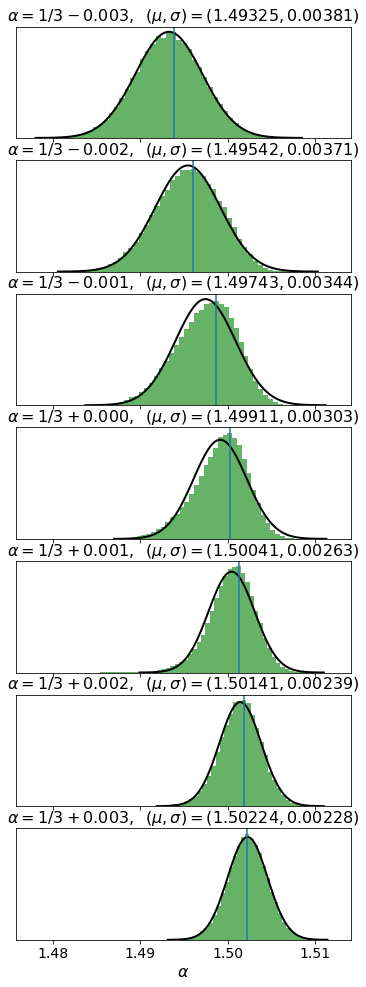
\includegraphics[width=0.5\textwidth]{cvar_boundary_behavior_discrete_0_1_2_shifting.png}
	\caption{Distribution of $\cvar_{\alpha}(L_n)$, with $n=10^5$, $X$ being the uniform distribution on $\{0, 1, 2\}$, as $\alpha$ crosses the $1/3$ boundary. Each histogram results from $10^5$ trials. Each black curve is the best fit normal distribution $\mathcal{N}(\mu, \sigma)$, with parameters $\mu, \sigma$ written above. Each vertical line denotes the estimated maximum of the distribution of $\cvar_\alpha(L_n)$. Notice how nearing $\alpha=1/3$, the fit to normal distribution degrades , and the estimated maximum shifts ahead.}
	\label{fig:cvar_boundary_behavior_discrete_0_1_2_shifting}
\end{figure}

\begin{figure}
	\centering
	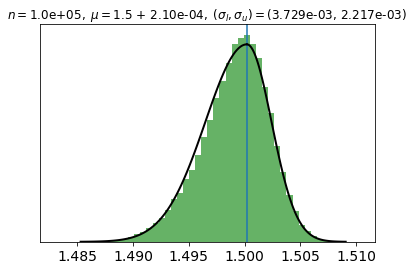
\includegraphics[width=0.6\textwidth]{cvar_boundary_behavior_discrete_0_1_2.png}
	\caption{Distribution of $\cvar_{1/3}(L_n)$, with $n=10^5$, $X$ being the uniform distribution on $\{0, 1, 2\}$. The histogram results from $10^5$ trials. The black curve is the best fit mixed normal distribution $\mathcal{N}(\mu, \sigma_l, \sigma_u)$, with $\mu = 1.5 + 2.1 \times 10^{-4}, \sigma_l = 0.003729, \sigma_u = 0.002217$, and the vertical line denotes the location of $\mu$. }
	\label{fig:cvar_boundary_behavior_discrete_0_1_2}
\end{figure}

\subsection{SLLN for \cvar}
\label{sec:slln_for_cvar}
Now we present the SLLN for the empirical process of \cvar assuming $X$ has finite variance. 

In \cite[Proposition 4.1]{acerbiCoherenceExpectedShortfall2002}, this is proved assuming only that $$\mathbb{E}((-X)^+)<\infty,$$
but the proof is more involved. 

\begin{theorem}[SLLN for \cvar]\label{thm:slln_cvar}
For any real random variable $X$ with finite variance, and any $\alpha\in[0, 1]$, then the empirical process of the $\cvar_\alpha$ of $X$ satisfies
\begin{equation}
\cvar_\alpha(L_n) \asconv \cvar_\alpha(X).
\end{equation}
\end{theorem}

\begin{proof} There are four cases to consider.
	
	1. If $\alpha = 0$, it is simply the SLLN for expectations.
	
	2. If $\alpha = 1$, it is proved in Theorem \ref{theorem:slln_esssup}.
	
	3. If $\alpha\in(0, 1)$, and $F_X^{-1}$ is continuous at $\alpha$, then the power series $K(t) = \mu(\alpha) t + \frac 12 \sigma(\alpha)^2 t^2 + o(t^2)$ in a neighborhood of $0$ means that $K$ is stricly convex and $C^2$ in that neighborhood. Now apply part (a) of Theorem \ref{theorem:gartner}.
	
	4. If $\alpha_0\in(0, 1)$, and $F_X^{-1}$ is not continuous at $\alpha_0$, then we prove by "squeezing with nearby points of continuity". 
	
	Since $F_X^{-1}$ is monotone, by Lebesgue's differentiation theorem \cite[Section 6.2]{roydenRealAnalysis2010}, it is almost everywhere differentiable. That is, let 
	$$D = \{x \in(0, 1): F_X^{-1} \text{ is differentiable at } x\}$$
	then $D$ has Lebesgue measure $1$.
	
	For any $\epsilon > 0$, since $\cvar_\alpha(X)$ is a continuous function of $\alpha$, there exists $\delta > 0$ such that 
	$$\forall\alpha \in(\alpha_0 - \epsilon, \alpha_0  + \epsilon), 
	|\cvar_\alpha(X) - \cvar_{\alpha_0}(X)| < \delta$$
	
	Now take $\alpha_1, \alpha_2 \in D\cap (\alpha_0 - \epsilon, \alpha_0  + \epsilon)$ such that $\alpha_1 < \alpha_0 < \alpha_2$. Note that $\alpha_1, \alpha_2$ exists because $D$ has measure $1$. 
	
	Then, by the SLLN for $\cvar_{\alpha_1}, \cvar_{\alpha_2}$, and the monotonicity of $\cvar_\alpha$ as a function of $\alpha$, we have 
	$$\limsup_n \cvar_{\alpha_0}(L_n) 
	\le \limsup_n \cvar_{\alpha_2}(L_n) \asconv \cvar_{\alpha_2}(X) 
	\le \cvar_{\alpha_0}(X) + \epsilon$$
	and similarly, 
	$$
	\liminf_n \cvar_{\alpha_0}(L_n) 
	\ge \cvar_{\alpha_0}(X) - \epsilon \text{ almost surely}
	$$
	Since for all $\epsilon > 0$, these two inequalities hold almost surely, we have, almost surely,
	$$\lim_n \cvar_{\alpha_0}(L_n) 
	= \cvar_{\alpha_0}(X).$$
\end{proof}

In fact, with a little manipulation, we immediately strengthen it to 
\begin{theorem}[Uniform SLLN for \cvar]
	\label{theorem:uni_slln}
	For any real random variable $X$ with finite variance, almost surely, for any $\alpha\in[0, 1]$, the empirical process of the $\cvar_\alpha$ of $X$ satisfies
	\begin{equation}
	\cvar_\alpha(L_n) \to \cvar_\alpha(X).
	\end{equation}
	that is, 
	\begin{equation}
		Pr\left(\forall \alpha\in[0, 1], \; \cvar_\alpha(L_n) \to \cvar_\alpha(X)\right) = 1
	\end{equation}
\end{theorem}
\begin{proof}
	Since for any particular $\alpha \in[0, 1]$, 
	$$\cvar_\alpha(L_n) \asconv \cvar_\alpha(X)$$
	so with probability one, it holds simultaneously for the countably many rational $\alpha\in[0, 1]$. Then by a "squeezing" argument like in the previous proof, it holds simultaneously for all $\alpha \in[0, 1]$:
	
	For any $\alpha \in (0, 1)$, and any $\epsilon > 0$, by continuity of $\cvar_\alpha$ with respect to $\alpha$, there exists rational $\alpha_1, \alpha_2 \in(0, 1)$, such that $\alpha_1 < \alpha < \alpha_2$, and 
	$$\cvar_{\alpha}(X) -\epsilon < \cvar_{\alpha_1}(X)\le \cvar_{\alpha}(X)\le \cvar_{\alpha_2}(X) < \cvar_{\alpha}(X) + \epsilon$$
	noting that $\cvar_{\alpha}(X)$ must be finite, since $X$ has finite expectation, and $\alpha < 1$. 
	
	Now, if $\cvar_{\alpha_i}(L_n) \to \cvar_{\alpha_i}(X)$ for $i = 1, 2$, then 
	$$\cvar_{\alpha}(X) -\epsilon \le \liminf_n \cvar_{\alpha}(L_n) $$
	$$\cvar_{\alpha}(X) +\epsilon \ge \limsup_n \cvar_{\alpha}(L_n) $$
	Since this holds for all $\epsilon > 0$, we have 
	$$\cvar_\alpha(L_n) \to \cvar_\alpha(X).$$
\end{proof}

\subsection{CLT of $\cvar_\alpha$ in the $\alpha \to 1$ limit}\label{sec:clt_right_tail}
Now we study the qualitative behavior of 
$$\sigma(\alpha)^2 = \mathbb{V}\left(\frac 1{\overbar\alpha} (X - F_X^{-1}(\alpha))^+\right)$$
at the $\alpha \to 1$ limit.

Let 
\begin{equation}
\
f(\alpha) = {\overbar\alpha} \sigma(\alpha) = \sqrt{\mathbb{V}\left( (X - F_X^{-1}(\alpha))^+\right)}
\end{equation}
then $f$ is a monotonically decreasing function of $\alpha \in (0, 1)$. 

At the $\alpha \to 0$ limit, 
$$f(\alpha) \to \sigma(0)^2 = \mathbb{V}(X).$$

The behavior of $f$ at the $\alpha \to 1$ limit depends on the right tail of the distribution of $X$. Qualitatively speaking, the thinner its right tail, the faster it approaches zero. Figure \ref{fig:schematic_cvar_tail} is a schematic plot of the behavior of $f$, for $X$ with tails of various thicknesses. 

The following examples are summarized by Table \ref{table:cvar_tail}.

\begin{table}[ht]
	\caption{The right tail of ${\overbar\alpha}\sigma(\alpha)$ in the $\alpha\to 1$ limit. The right tail of $\rho$ is either the $x\to \infty$ or the $x\to 0$ limit. As the right tail of $\rho$ becomes thinner, the right tail of ${\overbar\alpha}\sigma(\alpha)$ converges to $0$ quicker.}
	\centering
	$\begin{tabu}{|c|c|}
	\hline
	\text{right tail of }\rho&\text{right tail of }{\overbar\alpha}\sigma(\alpha)\\
	\hline
	\frac{1}{x^{3+\epsilon}}&{\overbar\alpha}^{\frac \epsilon 4}\\ 
	\frac{1}{x^{n}}, (n > 3)&{\overbar\alpha}^{\frac{n-3}{2n-2}}\\ 
	\frac{1}{x^{1001}}&{\overbar\alpha}^{0.499}\\ 
	e^{-x}& {\overbar\alpha}^{0.5}\\ 
	e^{-x^2/2}& \frac{\sqrt{{\overbar\alpha}}}{\erfc^{-1}(2{\overbar\alpha})}\\ 
	(-x)^{999}&{\overbar\alpha}^{0.5005}\\
	(-x)^n, (n > -1)&{\overbar\alpha}^{\frac{n+3}{2n+2}}\\ 
	(-x)^1&{\overbar\alpha}\\ 
	(-x)^0&{\overbar\alpha}^{1.5}\\ 
	(-x)^{-1+\epsilon}&{\overbar\alpha}^{\frac{1}{\epsilon}}\\
	\hline
	\end{tabu}$
	
\label{table:cvar_tail}
\end{table}


Now we list some examples, some of which are shown in Figure \ref{fig:cvar_stds}

\begin{ex}
	Suppose $X$ is uniform on $\{0, 1, 2\}$, then
	\begin{equation}
	\sigma(\alpha)^2 = \begin{cases}
		\frac{2}{3{\overbar\alpha}^2}\text{ if } \alpha\in [0, 1/3)\\
		\frac{2}{9{\overbar\alpha}^2} \text{ if } \alpha\in (1/3, 2/3)\\
		0 \text{ if } \alpha\in (2/3, 1)\\
	\end{cases}
	\end{equation}
	as shown in Figure \ref{fig:discrete_0_1_2_std}.
\end{ex}

\begin{ex}
	Suppose $X$ has a right tail of the form 
	$$\rho(x) \approx \frac{A}{x^n}$$
	where $n > 3$ to ensure that $X$ has finite variance, and $A> 0$ is an unspecified constant, then at the $\alpha \to 1$ limit, approximately 
	\begin{equation}
	\sigma(\alpha)^2 \propto \frac{1}{{\overbar\alpha}^2 \left(-\ln{\overbar\alpha}\right)^{n-3}}
	\end{equation}
	giving $f(\alpha) \propto \left(-\ln{\overbar\alpha}\right)^{-(n-3)/2}$ at $\alpha \to 1$ limit.
\end{ex}

\begin{ex}
	The exponential distribution with PDF 
	$$\rho(x) = \lambda e^{-\lambda x}, x > 0, \lambda > 0$$
	has 
	\begin{equation}
		\sigma(\alpha)^2 = \frac{1}{\lambda^2}\frac{1+\alpha}{1-\alpha}
	\end{equation}
	giving $f(\alpha) \propto {\overbar\alpha}^{1/2}$ at the $\alpha \to 1$ limit. See Figure \ref{fig:exp_std}.
\end{ex}

\begin{ex}
	The Gaussian distribution with PDF 
	$$\rho(x) = \frac{1}{\sqrt{2\pi}}e^{- x^2/2}$$
	has 
	\begin{equation}
	\sigma(\alpha)^2 = \frac{1}{{\overbar\alpha}^2}
	\left(
		1 + \alpha \phi(a)^2 
		+ \frac{\rho(\phi(\alpha))}{\overbar\alpha}((1 -2\alpha)\phi(\alpha) - \rho(\phi(\alpha)))
	\right)
	\end{equation}
	where 
	$$\phi(\alpha) = F_X^{-1}(\alpha) = \sqrt{2} \erf^{-1}(2\alpha - 1)$$
	is its quantile function, where $\erf$ is the error function defined by 
	\begin{equation}
		\erf(x) = 1- \frac{2}{\sqrt{\pi}} \int_{x}^{\infty} e^{-t^{2}} dt
	\end{equation}
	
	At the $\alpha \to 1$ limit, this gives 
	\begin{equation}
	f(\alpha) \approx \frac{\sqrt{{\overbar\alpha}}}{\erfc^{-1}(2{\overbar\alpha})}.
	\end{equation}
	Here, $\erfc$ is the complementary error function, defined by 
	\begin{equation}
	\erfc(x) = 1- \erf(x)
	\end{equation}
	 See Figure \ref{fig:gaussian_std}.
\end{ex}

\begin{ex}
	If $X$ is bounded above, shift it so that $\esssup(X) = 0$. Then suppose it has a PDF $\rho$,
	$$\rho(x) \approx A(-x)^n, x \in (-\epsilon, 0)$$
	where $n > -1$, and $A$ being an unspecified positive constant, then at the $\alpha \to 1$ limit, approximately
	\begin{equation}
	f(\alpha)\propto {\overbar\alpha}^{\frac{n+3}{2n+2}} 
	\end{equation}
	Notably, when $n=1$, $f(\alpha)\propto {\overbar\alpha}$, so $\sigma(\alpha) \propto 1$ in fact converges to a positive constant. This is shown in Figure \ref{fig:parabolic_std}. 
	
	When $ n > 1$, $\sigma(\alpha)$ diverges to infinity, and when $-1 < n < 1$, it converges to $0$. For example, when $X$ is uniform, it has $n=1$, and indeed by Equation \ref{eq:uniform_std}, $\lim_{\alpha \to 1}\sigma(\alpha) = 0$.
\end{ex}

\begin{ex}
	A particularly flat $\sigma(\alpha)$ that we found is shown in Figure \ref{fig:xex2_std}, defined by a real random variable with PDF
	$\rho(x) = -xe^{x^2/2}$, with $x < 0$. It gives
	\begin{equation}
	f(\alpha) = 2({\overbar\alpha} + \alpha^2 F(\sqrt{\ln \alpha})^2)
	\end{equation}
	where $F$ is the Dawson F function defined by
	\begin{equation}
	F(x) = e^{-x^2} \int_0^x e^{t^2} dt.
	\end{equation}
\end{ex}

\begin{figure}
	\centering
	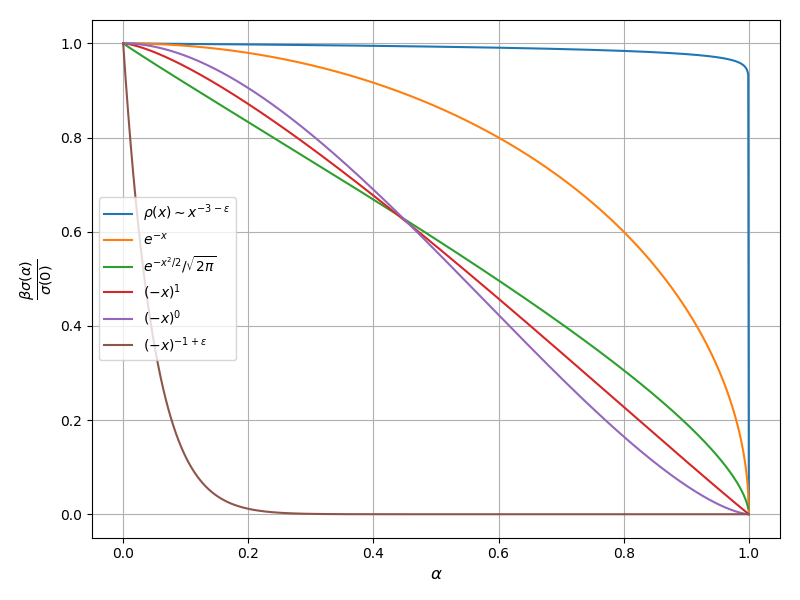
\includegraphics[width=\textwidth]{schematic_cvar_tail.png}
	\caption{Schematic drawing of the tail behavior of ${\overbar\alpha}\sigma(\alpha)$ for various distributions of $X$. In general, the thinner the tail, the faster it converges to $0$.\\
	Each legend lists the right tail of the density the $X$ corresponding to each curve. From top to bottom, the right tails of $X$ and of ${\overbar\alpha}\sigma(\alpha)$ grow thinner together.}
	\label{fig:schematic_cvar_tail}
\end{figure}


\section{Limit theorems for other risk measures}
It is natural to ask whether there are limit theorems for more general risk measures than \cvar. However, a literature search turned up nothing. As such, we believe the following results are new.

\subsection{SLLN for spectral risk measures}
When $X$ is bounded above and below, the uniform SLLN for \cvar can be extended to all spectral risk measures:

\begin{theorem}[uniform SLLN for spectral risk measures]
	\label{thm:uniform_slln_spec}
	Let $X\in \LL^\infty$, that is, it is a random variable with bounded range. Then almost surely, for any probability measure $m$ on $[0, 1]$, the spectral risk measure $\mathcal{F} = \int_0^1 \cvar_\alpha dm(\alpha)$ satisfies a SLLN:
	\begin{equation}
		\mathcal{F}(L_n)\to \mathcal{F}(X)
	\end{equation}
\end{theorem}
\begin{proof}
	Let $M > |X|$ be an upper bound of $X$, then by monotonicity of \cvar, 
	$$-M < \cvar_\alpha(L_n) < M, \; |\cvar_\alpha(L_n)| \le M $$
	By theorem \ref{theorem:uni_slln}, almost surely, $\cvar_\alpha(L_n)$ converges pointwise (with respect to $\alpha$) to $\cvar_\alpha(X)$. Then since $\int M dm(\alpha) = M$ is finite, by Lebesgue's dominated convergence theorem, 
	$$\lim_n\mathcal{F}(L_n) = \lim_n \int \cvar_\alpha(L_n)dm(\alpha) =  \int \cvar_\alpha(X)dm(\alpha) = \mathcal{F}(X)$$
\end{proof}

\subsection{CLT for spectral risk measures?}
In the proof of SLLN for spectral risk measures, the crucial step is using a SLLN of $\cvar_\alpha$ that holds uniformly over all $\alpha\in[0, 1]$. Analogously, we suspect that there is a CLT for spectral risk measures that depends on a uniform CLT, similar to results collected in \cite{dudleyUniformCentralLimit1999}.

In particular, we suspect that a proof can be found through the generalized Berry--Esseen Theorem for \cvar, as \cite[Theorem 1.1]{gaoAsymptoticBehaviorEmpirical2011}:

\begin{theorem}[Berry--Esseen theorem for \cvar]
	Given real random variable $X$ with finite third moment, $\alpha \in (0, 1)$, such that $\sigma(\alpha) > 0$, and $X$ has a strictly positive, continuous PDF in a neighborhood of $F^{-1}(\alpha)$, then there exists some $C_\alpha > 0$ such that
	\begin{equation}
	\|G_n-\Phi\|_\infty \le \frac{C_\alpha}{\sqrt{n}}
	\end{equation} 
	for all $n \in \mathbb{N}$, where $G_n$ is the CDF of the random variable 
	$$\frac{\sqrt n}{\sigma(\alpha)}(\cvar_\alpha(L_n) - \cvar_\alpha(X))$$
\end{theorem}

However, using the Berry--Esseen theorem, we were unable to prove the suspected generalization to the CLT of \cvar, so we leave it as a conjecture:
\begin{conj}[CLT for spectral risk measures]\label{conj:clt_spec}
	For any probability measure $m$ on $[0, 1]$, define a spectral risk measure $\mathcal{F} = \int_0^1 \cvar_\alpha dm(\alpha)$, then for any real random variable $X$ with finite variance, 
	\begin{equation}
	\sqrt{n}(\mathcal{F}(L_n) - \mathcal{F}(X)) \distconv \mathcal{N}(0, \sigma)
	\end{equation}
	for some $\sigma \ge 0$, provided that there does not exist some $\alpha_0\in[0, 1]$, such that $m(\alpha_0) > 0$, and $\sigma(\alpha)$ is discontinuous at $\alpha_0$, where $\sigma(\alpha)$ is the standard deviation of the limit distribution in Equation \ref{eq:clt_cvar_distconv}:
	$$\sqrt{n}(\cvar_\alpha(L_n) - \cvar_\alpha(X)) \distconv \mathcal{N}\left(0, \sigma(\alpha)\right)$$
	
	Otherwise, there exists $\sigma_1 > \sigma_2 \ge 0$ such that 
	\begin{equation}
	\sqrt{n}(\mathcal{F}(L_n) - \mathcal{F}(X)) \distconv \mathcal{N}_{mixed}(0, \sigma_1, \sigma_2)
	\end{equation}
\end{conj}

\subsection{CLT for entropic value at risk?}

Other than \cvar, another example of CRM is the entropic value at risk (\evar), proposed in \cite{ahmadi-javidEntropicValueatriskNew2012}.

\begin{defn}
	\label{defn:evar}
	For any $\alpha \in [0, 1]$, and real random variable $X$, its $\alpha$-level \evar is
	\begin{equation}
	\label{eq:evar_def}
	\evar_\alpha (X) = \inf_{t>0} \frac 1 t \ln\mathbb{E}\left(\frac{1}{1-\alpha}e^{tX}\right)
	\end{equation}
\end{defn}

%The dual representation of \evar is \cite[Theorem 4.9]{ahmadi-javidAnalyticalStudyNorms2017}
%\begin{equation}
%\mathscr{Q}_\alpha = \left\{Z : \mathbb{E} Z=1, Z \geq 0 \text{ and } \mathbb{E} Z \log Z \leq \log \frac{1}{1-\alpha}\right\}
%\end{equation}

The entropic value at risk (\evar) is similar to \cvar, and as such we have reasons to suspect it to have a similar CLT. We attempted to calculate the cumulant generating function for the empirical process of \evar, but without success. 


While having no definitive proof, numerical simulation strongly suggests that there exists a similar CLT for \evar:
\begin{conj}[CLT for EVaR]\label{conj:clt_evar}
Given any $X$ with finite variance, and any $\alpha\in [0, 1)$, its empirical process $L_n$ satisfies
\begin{equation}
	\sqrt{n}(\evar_\alpha(L_n) - \evar_\alpha(X)) \distconv \mathcal{N}(0, \sigma(\alpha))
\end{equation}
where $\sigma(\alpha)$ is a continuous function satisfying $\sigma(0)^2 =\mathbb{V}(X)$. 
\end{conj}

Figure \ref{fig:evar_discrete_0_1_2} plots the mean and standard deviation (normalized by $\sqrt{n}$) of the $\evar_\alpha(L_n)$, while Figure \ref{fig:evar_discrete_0_1_2_clt} shows that as $n\to \infty$, the distribution of $\evar_\alpha(L_n)$ becomes closer to normal distribution.

As shown in Figure \ref{fig:evar_discrete_0_1_2}, numerical calculation does not reveal any discontinuity of $\sigma(\alpha)$, akin to that of \cvar, suggesting that for \evar, the CLT holds for all $\alpha\in[0, 1)$.

\begin{figure}
	\centering
	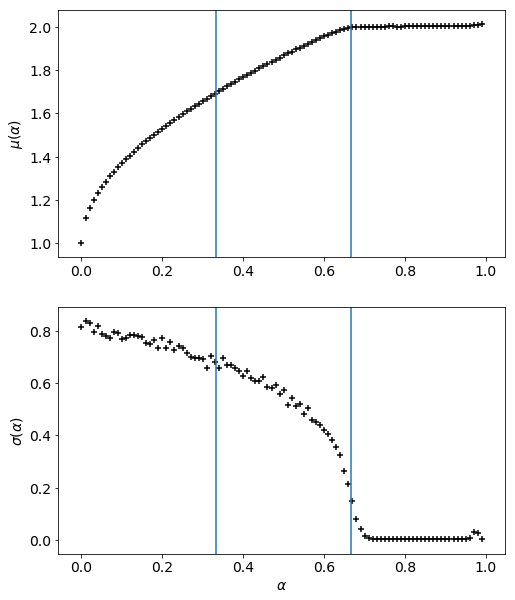
\includegraphics[width=0.7\textwidth]{evar_discrete_0_1_2.png}
	\caption{Mean and standard deviation (normalized by $\sqrt n$) of $\evar_\alpha(L_n)$ plotted as functions of $\alpha$, with $n=1000$, and $X$ being the uniform distribution on $\{0, 1, 2\}$. Each point is calculated from $1000$ trials. The two vertical lines denote $\alpha = 1/3, 2/3$ respectively. As apparent from the graph, $\sigma$ is a continuous function over $[0, 1]$, and equals zero for $\alpha > 2/3$. The blip at the right end of $\sigma(\alpha)$ is due to numerical instability of the root-finding algorithm, which is required in the calculation of $\evar$, as it involves searching for the infimum of a transcendental function, an infimum with no closed form. (see Equation \ref{eq:evar_def}).}
	\label{fig:evar_discrete_0_1_2}
\end{figure}

\begin{figure}
	\centering
	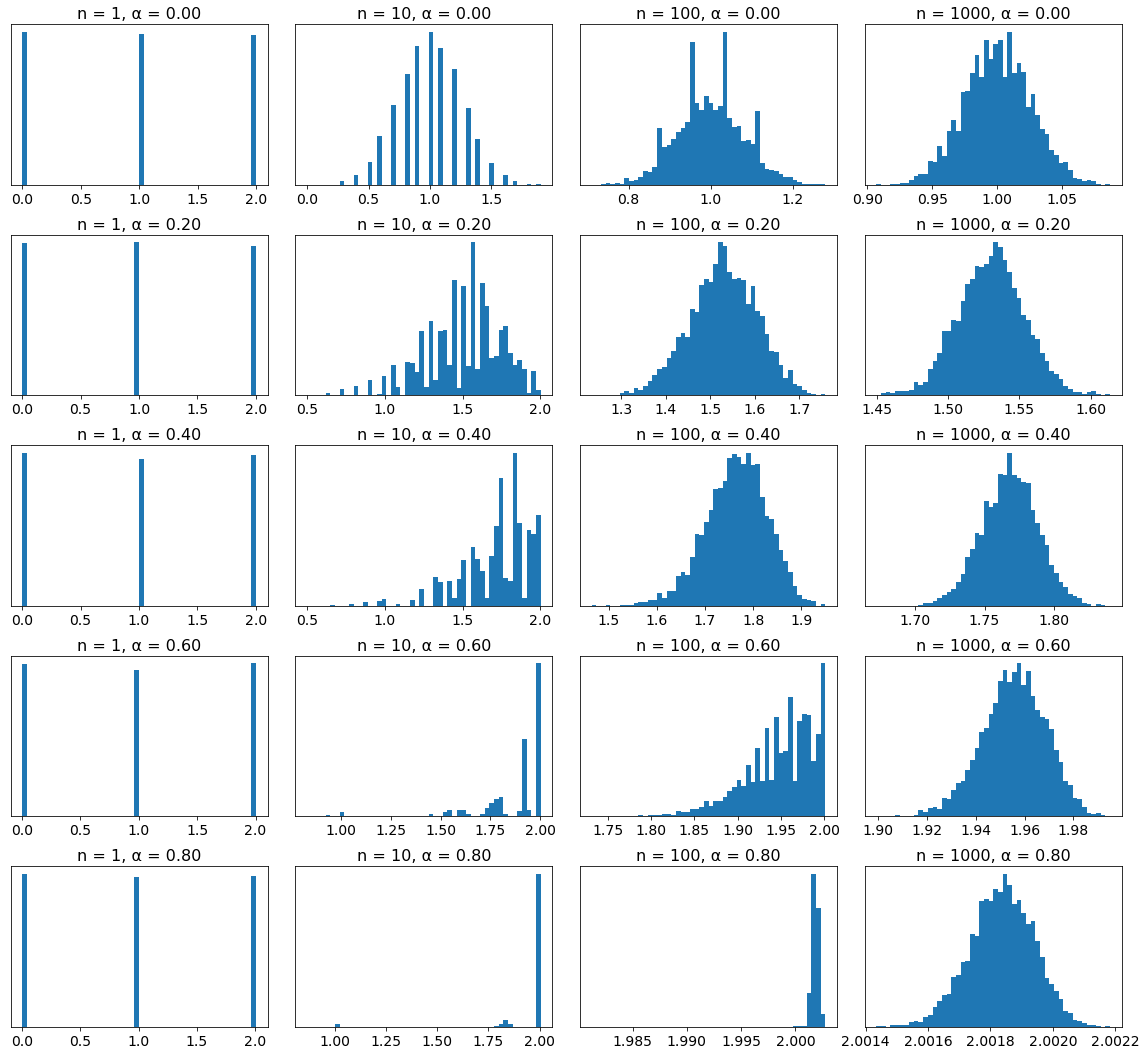
\includegraphics[width=\textwidth]{evar_discrete_0_1_2_clt.png}
	\caption{A demonstration of the CLT for \evar. Here, $X$ is the uniform distribution on $\{0, 1, 2\}$, and the PDF of $\evar_\alpha (L_n)$ plotted as a function of $n$ and $\alpha$. As $n$ increases, the distributions converge to normal distributions. Note that when $\alpha = 0.8$, the distribution becomes close to degenerate, as expected if $\sigma(\alpha) = 0$ when $\alpha > 2/3$. 
	Each histogram is the result of $5000$ trials. The x-axis is shifted and scaled in each plot to make the bell-shape apparent.}
	\label{fig:evar_discrete_0_1_2_clt}
\end{figure}


  
\chapter{Conclusion}
\label{chapter_conclusion}
In this chapter, we enumerate our main results, conjectures, sketch out applications to machine learning, and further research directions.

\section{Summary of results and conjectures}
Unless otherwise noted, all generalizations that follow are from expectation to coherent risk measures.

In Chapter \ref{chapter_finite_dimensional}, we showed:
\begin{enumerate}
	\item The geometric-analytic correspondence of risk measures with their envelope representations (Proposition \ref{prop:envelop_rep}).
	\item The formula (without proof) for envelope representation of CVaR (Equation \ref{eq:env_cvar}).
	\item Kusuoka representation theorem on finite uniform sample spaces (Section \ref{sec:uniform_space}).
	\item Counterexamples to Kusuoka representation theorem on finite nonuniform sample spaces (Section \ref{sec:nonuniform_space}).
\end{enumerate}

In Chapter \ref{chapter_inequalities}, we showed:
\begin{enumerate}
	\item Generalizations of (Section \ref{sec:elementary_inequalities}).
	\item Generalizations of concentration inequalities (Section \ref{sec:tail_ineq}).
	\item Generalizations, from expectation to spectral risk measures, of basic concepts (Section \ref{sec:slt_cvar}) and the fundamental theorem (Theorem \ref{theorem:funtheo_slt_2}) in statistical learning theory.
\end{enumerate}
We conjectured the CVaR law of total expectations (Conjecture \ref{conj:total_cvar}).

In Chapter \ref{chapter_clt}, we showed:
\begin{enumerate}
	\item The uniform strong law of large numbers (SLLN) for spectral risk measures (Theorem \ref{thm:uniform_slln_spec}), whic subsumes the SLLN for spectral risk measures and the SLLN for CVaR (Theorem \ref{theorem:uni_slln}).
	\item The central limit theorem (CLT) for CVaR (Theorem \ref{theorem:clt_cvar}).
	\item Examples of the CLT for CVaR of exemplar random variables (Section \ref{sec:clt_right_tail}).
\end{enumerate} 
We conjectured: 
\begin{enumerate}
	\item A "mixed" CLT for CVaR (Conjecture \ref{conj:mixed_gaussian}).
	\item A CLT for spectral risk measures (Conjecture \ref{conj:clt_spec}).
	\item A CLT for entropic value at risk (Conjecture \ref{conj:clt_evar}).
\end{enumerate} 


\section{Machine learning applications}
The stated goal of the thesis is to investigate consequences of generalizing probability theory by replacing expectation with coherent risk measures, especially \cvar, but such general investigations are not the original motivation of the authors. We were drawn to this topic from considering the use of probability in machine learning.

As in the very first page of the thesis, many machine learning problems can be cast into the form of risk minimization. Risk is often defined as the expectation of loss. By replacing expectation with CVaR or other coherent risk measures, we can obtain a risk-management tuning knob on machine learning algorithms.

In \cite{tamarOptimizingCVaRSampling2015}, a stochastic gradient descent algorithm for $\cvar_{0.05}$ is used to train a Tetris-playing program that, instead of minimizing the expectation of loss (the negative of score), minimizes the $\cvar_{0.05}$ of loss. It was found that, compared to a loss-minimizing agent, this agent was less likely to attempt high-risk high-reward Tetris maneuvers.

In \cite{chowRisksensitiveRobustDecisionmaking2015}, the authors described algorithms for solving Markov Decision Problems, optimized to minimize the CVaR risk measure, instead of the expectation. They derived theoretical error bounds to their algorithms, and tested the algorithm in a car navigating through a field with obstacles. As expected, a CVaR-optimizing agent drove more cautiously than the original expectation-optimizing agent.

In \cite{chowAlgorithmsCVaROptimization2014}, the authors proposed the actor-critic algorithm for reinforcement learning, so that it minimizes the CVaR risk measure, instead of the expectation. They proved its convergence properties, and applied it to an investment problem. Its behavior was found to be more risk-averse than the original expectation-optimizing algorithm.

In \cite{maurerEmpiricalBernsteinBounds2009}, the empirical risk minimization (ERM) learning algorithm is generalized by adding to the expectation of loss with a variance term, essentially generalizing ERM by replacing expectation with a non-convex risk measure. \cite{namkoongVariancebasedRegularizationConvex2017a} continues the work by proposing a similarly non-convex risk measure that is more computationally efficient, has faster rates of convergence than empirical risk minimization. The authors also demonstrated its performance on two classification problems.

In \cite{majumdarRisksensitiveInverseReinforcement2017}, CRM is applied to the problem of inverse reinforcement learning, wherein a learning agent observed humans playing a driving game, and inferred what preferences humans have from their behavior. It was found that each human's behavior was well-modeled by minimization of their own CRM, which differs between humans. Some humans have CRM that are very sensitive to variations, which corresponds to their highly risk-averse driving behavior. Other humans have CRM close to expectation, which corresponds to their highly risk-neutral driving behavior.

In \cite{williamsonFairnessRiskMeasures2019a}, the problem of fair machine learning is discussed. The authors proposed to define \textit{fairness risk measures}, which are special cases of CRM, and demonstrated a tradeoff between fairness and accuracy, that is, a supervised-learning algorithm minimizing fairness risk, instead of loss expectation, gradually became less accurate as the fairness risk increasingly weights fairness over loss minimization. See also Section 5.3 of the same paper for more technical applications of CRM in machine learning.

\section{Further research directions}
We propose that future research in general risk measures can include: 
\begin{enumerate}
	\item The resolution of conjectures proposed in the paper.
	\item Generalization of more advanced probabilistic and statistical inequalities, such as McDiarmid's inequality, to general risk measures.
	\item Demonstration of benefit of using general risk measures in a practical, large-scale machine-learning application.
	\item Collaboration between experts on the many aspects of risk, such as financial mathematicians, engineers with expertise in reliability engineering, legal theorists who deal with risks in law (such as tort law), machine learning practitioners, and psychologists who study human perceptions of risk.
\end{enumerate}



% APPENDICES


  % change chapter name and counters (eg Chapter 1 -> Appendix A)
  \appendix


  % assuming there are files appendix1.tex etc...
  %
\chapter{Endnotes}
\label{appendix_endnotes}

  %\include{appendix2}
  %\include{appendix3}
  %etc




% BIBLIOGRAPHY


  % add Bibliography to table of contents
  \addcontentsline{toc}{chapter}{Bibliography}


  % list BibTeX (.bib) files and choose bibliography style

  % OR... do it manually in the file bibliography.tex
  \printbibliography



\end{document}
